\pdfpagewidth = 8.5in
\pdfpageheight = 11.0in
\usepackage[left=1in,right=1in,top=1in,bottom=1in]{geometry}

\pagestyle{plain}
\pagenumbering{arabic}
\usepackage{setspace}
\usepackage[usenames]{color}
\usepackage[fleqn]{amsmath}
\usepackage{amssymb}
\usepackage{graphicx}
\usepackage{url}
\usepackage{verbatim}
\usepackage{appendix}
\usepackage{indentfirst}
\usepackage{booktabs}
\usepackage{multirow}
\usepackage[table, x11names]{xcolor}
\usepackage{ragged2e}
\usepackage{upgreek}
\usepackage{lscape}
\usepackage{longtable}
\usepackage[flushleft, referable]{threeparttablex}
\usepackage{rotating}
\usepackage[T1]{fontenc}
\usepackage[titles]{tocloft}
\usepackage{xspace}
\usepackage{ifthen}
\usepackage{cancel}
\usepackage{rotating}
\usepackage{array}
\usepackage{tabulary}
\usepackage{authblk}

\usepackage{hyperref}
\hypersetup{pdfborder={0 0 0}, colorlinks=true, urlcolor=black, linkcolor=black, citecolor=black}
\usepackage[capitalize]{cleveref}
\newcommand{\crefrangeconjunction}{--}

\usepackage[right, mathlines]{lineno}
\setlength\linenumbersep{1cm}
\def\linenumberfont{\normalfont\scriptsize\sffamily}

% \usepackage[format=plain, labelsep=period, justification=raggedright, singlelinecheck=true, skip=2pt, font=sf]{caption}
\usepackage{caption}
\DeclareCaptionLabelFormat{noSpace}{{#1}{#2}}
\DeclareCaptionListFormat{figList}{Figure {#2}.}
\DeclareCaptionListFormat{sFigList}{Figure S{#2}.}
\usepackage{subfig}

%\DeclareMathSizes{12}{12}{7}{5}

% \usepackage[round]{natbib}

% \makeatletter
%   \renewcommand{\section}{\@startsection{section}{1}{0mm}%
%     {-12pt}%
%     {12pt}%
%     {\sffamily\LARGE\itshape}}
% \makeatother

% \makeatletter
%   \renewcommand{\subsection}{\@startsection{subsection}{1}{0mm}%
%   {-10pt}%
%   {4pt}%
%   {\sffamily\large\bfseries\MakeUppercase}}
% \makeatother

% \makeatletter
%   \renewcommand{\subsubsection}{\@startsection{subsubsection}{1}{0mm}%
%   {-10pt}%
%   {10pt}%
%   {\sffamily\large\itshape}}
% \makeatother

% make list of figures ragged right
% \makeatletter
%   \renewcommand{\@tocrmarg}{0cm plus1fil}
% \makeatother

\setlength\linenumbersep{1cm}

% \newcommand{\change}[1]{{\color{blue} #1}\xspace}
\newcommand{\change}[1]{{\color{black} #1}\xspace}


\newcommand{\citationNeeded}{\textcolor{magenta}{\textbf{[CITATION NEEDED!]}}\xspace}
\newcommand{\tableNeeded}{\textcolor{magenta}{\textbf{[TABLE NEEDED!]}}\xspace}
\newcommand{\figureNeeded}{\textcolor{magenta}{\textbf{[FIGURE NEEDED!]}}\xspace}
\newcommand{\highLight}[1]{\textcolor{magenta}{\MakeUppercase{#1}}}

\newcommand{\editorialNote}[1]{\textcolor{red}{[\textit{#1}]}}
\newcommand{\ignore}[1]{}
\newcommand{\addTail}[1]{\textit{#1}.---}
\newcommand{\super}[1]{\ensuremath{^{\textrm{#1}}}}
\newcommand{\sub}[1]{\ensuremath{_{\textrm{#1}}}}
\newcommand{\dC}{\ensuremath{^\circ{\textrm{C}}}}

\providecommand{\e}[1]{\ensuremath{\times 10^{#1}}}

\newcommand{\mthnote}[2]{{\color{red} #2}\xspace}
\newcommand{\cwlnote}[2]{{\color{orange} #2}\xspace}

\newcommand{\ifTwoArgs}[3]{\ifthenelse{\equal{#1}{}\or\equal{#2}{}}{}{#3}\xspace}
\newcommand{\ifArg}[2]{\ifthenelse{\equal{#1}{}}{}{#2}\xspace}

%% New notation for divergence times
\newcommand{\divTime}[1]{\ensuremath{\tau_{#1}}\xspace}
\newcommand{\divTimeVector}{\ensuremath{\boldsymbol{\divTime{}}}\xspace}
\newcommand{\divTimeIndex}[1]{\ensuremath{t_{#1}}\xspace}
\newcommand{\divTimeIndexVector}{\ensuremath{\mathbf{\divTimeIndex{}}}\xspace}
\newcommand{\divTimeMap}[1]{\ensuremath{T_{#1}}\xspace}
\newcommand{\divTimeMapVector}{\ensuremath{\mathbf{\divTimeMap{}}}\xspace}
\newcommand{\divTimeScaled}[2]{\ensuremath{\mathcal{T}_{#1\protect\ifTwoArgs{#1}{#2}{,}#2}}\xspace}
\newcommand{\divTimeScaledVector}{\ensuremath{\mathbf{\divTimeScaled{}{}}}\xspace}
\newcommand{\divTimeMean}{\ensuremath{\bar{\divTimeMap{}}}\xspace}
\newcommand{\divTimeVar}{\ensuremath{s^{2}_{\divTimeMap{}}}\xspace}
\newcommand{\divTimeDispersion}{\ensuremath{D_{\divTimeMap{}}}\xspace}
\newcommand{\divTimeNum}{\ensuremath{\lvert \divTimeVector \rvert}\xspace}
\newcommand{\demographicParams}[1]{\ensuremath{\Theta_{#1}}\xspace}
\newcommand{\demographicParamVector}{\ensuremath{\mathbf{\demographicParams{}}}\xspace}
\newcommand{\popSampleSize}[2]{\ensuremath{n_{#1\protect\ifTwoArgs{#1}{#2}{,}#2}}}
\newcommand{\gammaShape}[1]{\ensuremath{a_{#1}}\xspace}
\newcommand{\gammaScale}[1]{\ensuremath{b_{#1}}\xspace}
\newcommand{\betaA}[1]{\ensuremath{a_{#1}}\xspace}
\newcommand{\betaB}[1]{\ensuremath{b_{#1}}\xspace}
\newcommand{\integerPartitionSet}[1]{\ensuremath{a({#1})}\xspace}
\newcommand{\integerPartitionNum}[1]{\ensuremath{\lvert \integerPartitionSet{#1} \rvert}\xspace}
\newcommand{\concentrationParam}{\ensuremath{\chi}\xspace}
\newcommand{\stirlingFirst}[2]{\ensuremath{c(#1, #2)}\xspace}
\newcommand{\descendantThetaMean}[1]{\ensuremath{\bar{\theta}_{D\protect\ifArg{#1}{,}#1}}\xspace}
\newcommand{\numPriorSamples}{\ensuremath{\mathbf{n}}\xspace}
\newcommand{\paramSampleVector}[1]{\ensuremath{\Lambda_{#1}}\xspace}
\newcommand{\paramSampleMatrix}{\ensuremath{\boldsymbol{\paramSampleVector{}}}\xspace}
\newcommand{\modelDPP}{\ensuremath{M_{DPP}}\xspace}
\newcommand{\modelDPPOrdered}{\ensuremath{M^{\circ}_{DPP}}\xspace}
\newcommand{\modelUniform}{\ensuremath{M_{Uniform}}\xspace}
\newcommand{\modelUshaped}{\ensuremath{M_{Ushaped}}\xspace}
\newcommand{\modelOld}{\ensuremath{M_{msBayes}}\xspace}
\newcommand{\priorDPP}[1]{\ensuremath{DP(\concentrationParam #1)}\xspace}
\newcommand{\priorUniform}{\ensuremath{DU\{\integerPartitionSet{\npairs{}}\}}\xspace}
\newcommand{\priorOld}{\ensuremath{DU\{1, \ldots, \npairs{}\}}\xspace}
\newcommand{\powerSeriesOld}{\ensuremath{\mathcal{M}_{msBayes}}\xspace}
\newcommand{\powerSeriesUniform}{\ensuremath{\mathcal{M}_{Uniform}}\xspace}
\newcommand{\powerSeriesExp}{\ensuremath{\mathcal{M}_{Exp}}\xspace}

\newcommand{\allDatasets}{\ensuremath{\mathcal{\alignment{}{}}}\xspace}
\newcommand{\allParameterValues}{\ensuremath{\boldsymbol{\Theta}}\xspace}
\newcommand{\bayesfactor}[2]{\ensuremath{BF_{#1\protect\ifArg{#2}{,}#2}}}
\newcommand{\given}{\ensuremath{\,|\,}\xspace}
\newcommand{\msb}{\upshape\texttt{\MakeLowercase{ms\MakeUppercase{B}ayes}}\xspace}
\newcommand{\abctoolbox}{\upshape\texttt{ABCtoolbox}\xspace}
\newcommand{\dppmsbayes}{\upshape\texttt{dpp-msbayes}\xspace}
\newcommand{\pymsbayes}{\upshape\texttt{PyMsBayes}\xspace}
\newcommand{\hky}{HKY85\xspace}
\newcommand{\uniformMin}[1]{\ensuremath{a_{#1}}\xspace}
\newcommand{\uniformMax}[1]{\ensuremath{b_{#1}}\xspace}
\newcommand{\locusRateHetShapeParameter}{\ensuremath{\alpha}\xspace}
\newcommand{\ancestralThetaVector}{\ensuremath{\boldsymbol{\theta_{A}}}\xspace}
\newcommand{\descendantThetaVector}[1]{\ensuremath{\boldsymbol{\theta_{D#1}}}\xspace}
\newcommand{\divtscaledvector}{\ensuremath{\mathbf{{\divtscaled{}{}}}}\xspace}
\newcommand{\divtvector}{\ensuremath{\boldsymbol{\divt{}}}\xspace}
\newcommand{\divtuniquevector}{\ensuremath{\mathbf{\divtunique{}}}\xspace}
\newcommand{\bottleTimeVector}{\ensuremath{\boldsymbol{\bottleTime{}}}\xspace}
\newcommand{\bottleTime}[1]{\ensuremath{\divt{B\ifArg{#1}{,}#1}}\xspace}
\newcommand{\bottleScalarVector}[1]{\ensuremath{\boldsymbol{\bottleScalar{#1}{}}}\xspace}
\newcommand{\bottleScalar}[2]{\ensuremath{\zeta_{D#1\protect\ifArg{#2}{,}#2}}\xspace}
\newcommand{\migrationRateVector}{\ensuremath{\mathbf{\migrationRate{}}}\xspace}
\newcommand{\geneTreeVector}{\ensuremath{\mathbf{\geneTree{}{}}}\xspace}
\newcommand{\alignmentVector}{\ensuremath{\mathbf{\alignment{}{}}}\xspace}
\newcommand{\alignment}[2]{\ensuremath{X_{#1\protect\ifTwoArgs{#1}{#2}{,}#2}}\xspace}
\newcommand{\geneTree}[2]{\ensuremath{G_{#1\protect\ifTwoArgs{#1}{#2}{,}#2}}\xspace}
\newcommand{\migrationRate}[1]{\ensuremath{m_{#1}}\xspace}
\newcommand{\recombinationRate}{\ensuremath{r}\xspace}
\newcommand{\ploidyScalar}[2]{\ensuremath{\rho_{#1\protect\ifTwoArgs{#1}{#2}{,}#2}}\xspace}
\newcommand{\ploidyScalarVector}{\ensuremath{\boldsymbol{\ploidyScalar{}{}}}\xspace}
\newcommand{\descendantRelativeThetaVector}[1]{\ensuremath{\boldsymbol{\eta_{D#1}}}\xspace}
\newcommand{\descendantRelativeTheta}[2]{\ensuremath{\eta_{D#1\protect\ifArg{#2}{,}#2}}\xspace}
\newcommand{\mutationRateScalarConstant}[2]{\ensuremath{\nu_{#1\protect\ifTwoArgs{#1}{#2}{,}#2}}\xspace}
\newcommand{\mutationRateScalarConstantVector}{\ensuremath{\boldsymbol{\mutationRateScalarConstant{}{}}}\xspace}
\newcommand{\locusMutationRateScalar}[1]{\ensuremath{\upsilon_{#1}}\xspace}
\newcommand{\locusMutationRateScalarVector}{\ensuremath{\boldsymbol{\upsilon}}\xspace}
\newcommand{\hkyModel}[2]{\ensuremath{\phi_{#1\protect\ifTwoArgs{#1}{#2}{,}#2}}\xspace}
\newcommand{\hkyModelVector}{\ensuremath{\boldsymbol{\hkyModel{}{}}}\xspace}
\newcommand{\mutationRate}{\ensuremath{\mu}\xspace}
\newcommand{\iid}{\textit{iid}\xspace}
\newcommand{\model}[1]{\ensuremath{\Theta}\xspace}
\newcommand{\npairs}[1]{\ensuremath{Y_{#1}}}
\newcommand{\nloci}[1]{\ensuremath{k_{#1}}\xspace}
\newcommand{\nlociTotal}{\ensuremath{K}\xspace}
\newcommand{\myTheta}[1]{\ensuremath{\theta_{#1}}}
\newcommand{\ancestralTheta}[1]{\ensuremath{\theta_{A\protect\ifArg{#1}{,}#1}}\xspace}
\newcommand{\descendantTheta}[2]{\ensuremath{\theta_{D#1\protect\ifArg{#2}{,}#2}}\xspace}
\newcommand{\meanDescendantTheta}[1]{\ensuremath{\descendantTheta{}{#1}}\xspace}
\newcommand{\nucdiv}[1]{\ensuremath{\pi_{#1}}}

\newcommand{\ssVector}[1]{\ensuremath{\mathbf{\alignmentSS{#1}{}}}\xspace}
\newcommand{\ssVectorObs}{\ensuremath{\ssVector{}^*}\xspace}
\newcommand{\ssSpace}{\ensuremath{\euclideanSpace{\ssVectorObs}}\xspace}
\newcommand{\ssVectorObsPLS}{\ensuremath{\ssVectorObs_{PLS}}\xspace}
\newcommand{\alignmentSS}[2]{\ensuremath{S_{#1\protect\ifTwoArgs{#1}{#2}{,}#2}}\xspace}
\newcommand{\alignmentSSObs}[2]{\ensuremath{\alignmentSS{#1}{#2}^*}\xspace}
\newcommand{\tol}{\ensuremath{\epsilon}\xspace}
\newcommand{\euclideanSpace}[1]{\ensuremath{B_{\tol}(#1)}\xspace}
\newcommand{\hpvector}[1]{\ensuremath{\Lambda_{#1}}}
\newcommand{\divtscaled}[2]{\ensuremath{t_{#1\protect\ifTwoArgs{#1}{#2}{,}#2}}}
\newcommand{\divt}[1]{\ensuremath{\tau_{#1}}}
\newcommand{\divtunique}[1]{\ensuremath{T_{#1}}}
\newcommand{\ssMatrix}{\ensuremath{\mathbb \alignmentSS{}{}}\xspace}
\newcommand{\ssMatrixRaw}[1]{\ensuremath{{\ssMatrix}_{stats#1}}\xspace}
\newcommand{\ssMatrixPLS}[1]{\ensuremath{{\ssMatrix}_{PLS#1}}\xspace}
\newcommand{\hpmatrix}[1]{\ensuremath{\mathcal{P}_{#1}}}
\newcommand{\meant}[2]{\ensuremath{E(\divt{#1})_{#2}}}
\newcommand{\meantestimate}{\ensuremath{\hat{E(\divt{})}}\xspace}
\newcommand{\vart}[2]{\ensuremath{Var(\divt{#1}{})_{#2}}}
\newcommand{\vmratio}[1]{\ensuremath{\Omega_{#1}}}
\newcommand{\numt}[1]{\ensuremath{\Psi_{#1}}}
\newcommand{\probnumt}[2]{\ensuremath{p(\numt{#1} = {#2})}}
\newcommand{\postprobnumt}[1]{\ensuremath{p(\numt{} = {#1}|\ssSpace)}}
\newcommand{\postprobnumtnot}[1]{\ensuremath{p(\numt{} \neq {#1}|\ssSpace)}}
\newcommand{\postprobomegasimult}{\ensuremath{p(\vmratio{} < 0.01 | \ssSpace)}\xspace}
\newcommand{\modelprior}[1]{\ensuremath{f(\model{})}}
\newcommand{\modelpost}[1]{\ensuremath{f(\model{}|\ssSpace)}}
\newcommand{\npriorsamples}{\ensuremath{n}\xspace}
\newcommand{\globalcoalunit}{\ensuremath{4\globalpopsize}\xspace}
\newcommand{\globalpopsize}{\ensuremath{N_C}\xspace}
\newcommand{\effectivePopSize}[1]{\ensuremath{N_e{#1}}\xspace}
\newcommand{\coalunit}{\ensuremath{4\effectivePopSize{}}\xspace}
\newcommand{\priorsample}[1]{\ensuremath{\hpmatrix{\modelprior{}}}}
\newcommand{\truncprior}[1]{\ensuremath{\hpmatrix{\tol}}\xspace}
\newcommand{\postsample}[1]{\ensuremath{\hpmatrix{\modelpost{}}}}
\newcommand{\abcllr}[1]{ABC\sub{LLR}}
\newcommand{\abcglm}[1]{ABC\sub{GLM}}
\newcommand{\integerPartition}[1]{\ensuremath{a({#1})}}
\newcommand{\uniqueModel}[2]{\ensuremath{M_{#1\protect\ifTwoArgs{#1}{#2}{,}#2}}}
\newcommand{\taxonLocusVector}[1]{\ensuremath{\{#1{1}{1},\ldots,#1{\npairs{}}{\nloci{\npairs{}}}\}}\xspace}
\newcommand{\taxonVector}[1]{\ensuremath{\{#1{1},\ldots,#1{\npairs{}}\}}\xspace}
\newcommand{\locusVector}[1]{\ensuremath{\{#1{1},\ldots,#1{\nlociTotal}\}}\xspace}

\newcommand{\validationAccuracyCaption}[2]{Estimation accuracy for model
    #2 when analyzing data generated under #1.
    A random sample of 5000 posterior estimates (from 50,000) are plotted,
    including both (A, B, \& C) unadjusted and (D, E, \&
    F) GLM-regression-adjusted estimates.
    Normal random variates ($N(0, 0.005)$) have been added to the estimates and
    true values of \divTimeNum (A \& D) to reduce overlap of plot symbols.
    The root mean square error (RMSE) calculated from the 5000 estimates is
    provided.}
\newcommand{\validationModelChoiceCaption}[2]{Model-choice accuracy for model
    #2 when analyzing data generated under #1.
    The estimated posterior probability of a single divergence event, based on
    (A \& C) $\divTimeNum = 1$ and (B \& D) $\divTimeDispersion < 0.01$, from
    50,000 posterior estimates are assigned to bins of width 0.05 and plotted
    against the proportion of replicates in each bin where the truth is
    $\divTimeNum = 1$ or $\divTimeDispersion < 0.01$.
    Results based on the (A \& B) unadjusted and (C \& D) GLM-adjusted
    posterior estimates are shown.}
\newcommand{\powerAccuracyCaption}[2]{Estimation accuracy for model
    #2 when analyzing data generated under the series of models #1.
    The true versus estimated value of the dispersion index of divergence
    times (\divTimeDispersion) is plotted for 1000 datasets simulated
    under each of the #1 models, and the proportion of estimates less
    than the truth, $p(\hat{\divTimeDispersion} < \divTimeDispersion)$,
    is shown for each data model.}
\newcommand{\powerPsiCaption}[2]{
    The power of model #2 to detect random variation in divergence times as
    simulated under the series of models #1.
    The plots illustrate the estimated number of divergence events
    ($\hat{\divTimeNum}$) from analyses of 1000 datasets simulated under each
    of the #1 models, with the the estimated probability of the model inferring
    one divergence event, $p(\hat{\divTimeNum} = 1)$, given for each data
    model.}
\newcommand{\powerDispersionCaption}[2]{
    The power of model #2 to detect random variation in divergence times as
    simulated under the series of models #1.
    The plots illustrate the estimated dispersion index of divergence times
    ($\hat{\divTimeDispersion}$) from analyses of 1000 datasets simulated under
    each of the #1 models, with the the estimated probability of the model
    inferring one divergence event, $p(\hat{\divTimeDispersion} < 0.01)$, given
    for each data model.}
\newcommand{\powerPsiProbCaption}[2]{
    The tendency of model #2 to support one divergence event when there is
    random variation in divergence times as simulated under the series of
    models #1.
    The plots illustrate histograms of the estimated posterior probability of
    the one divergence model, $p(\divTimeNum = 1 | \ssSpace)$, from analyses of
    1000 datasets simulated under each of the #1 models, with the the estimated
    probability of the model strongly supporting one divergence event,
    $p(BF_{\divTimeNum = 1, \divTimeNum \neq 1} > 10)$, given for each data
    model.}
\newcommand{\powerDispersionProbCaption}[2]{
    The tendency of model #2 to support one divergence event when there is
    random variation in divergence times as simulated under the series of
    models #1.
    The plots illustrate histograms of the estimated posterior probability of
    the one divergence model, $p(\divTimeDispersion < 0.01 | \ssSpace)$, from
    analyses of 1000 datasets simulated under each of the #1 models, with the
    the estimated probability of the model strongly supporting one divergence
    event, $p(BF_{\divTimeDispersion < 0.01, \divTimeDispersion \geq 0.01} >
    10)$, given for each data model.}
\newcommand{\simulationDescription}[2]{\change{Each plot represents #1
    simulation replicates using the same $#2$ samples from the prior}}
\newcommand{\simulationDistribution}{\ensuremath{\divt{} \sim U(0,
    \divt{max})}\xspace}
\newcommand{\estimateDescription}[2]{All estimates were obtained using #1 and #2}
\newcommand{\estimateDescriptionUncorrected}[1]{All estimates based on
    unadjusted posterior, \truncprior{}, obtained using #1}
\newcommand{\priorDescription}[4]{Prior settings were \priorSettings{#1}{#2}{#3}{#4}}
\newcommand{\priorSettings}[4]{$\divt{} \sim U(0, #1)$,
    $\meanDescendantTheta{} \sim U(#2, #3)$, and
    $\ancestralTheta{}{} \sim U(#2, #4)$}
\newcommand{\priorDescriptionBug}[4]{Prior settings were
    \priorSettingsBug{#1}{#2}{#3}{#4}}
\newcommand{\priorSettingsBug}[4]{$\divt{} \sim U(0, #1)$,
    $\meanDescendantTheta{} \sim U(#2, #3)$, and
    $\ancestralTheta{}{} \sim U(0.01, #4)$}
\newcommand{\simulationScheme}{simulations where \divt{} (in \globalcoalunit
    generations) for 22 population pairs is drawn from a series of uniform
    distributions, \simulationDistribution}
\newcommand{\captionPowerOmega}{Histograms of the estimated dispersion index
    of divergence times ($\hat{\vmratio{}}$) from \simulationScheme.
    The threshold for one divergence event \citep{Hickerson2006} is indicated
    by the dashed line, and the estimated probability of inferring one
    divergence event, $p(\hat{\vmratio{}}\le 0.01)$, is given for each
    \divt{max}}
\newcommand{\captionPowerPsiMode}{Histograms of the estimated number of
    divergence events ($\hat{\numt{}}$) from \simulationScheme.
    The estimated probability of inferring one divergence event,
    $p(\hat{\numt{}} = 1)$, is given for each \divt{max}}
\newcommand{\captionPowerPsi}{Histograms of the estimated posterior
    probability of one divergence event, \postprobnumt{1}, from
    \simulationScheme.
    The estimated probability of inferring one divergence event with a
    Bayes factor greater than 10 (dashed black line),
    $p(\bayesfactor{\numt{}=1}{\numt{} \ne 1} > 10)$, is given for each \divt{max}.
    The red line indicates $\postprobnumt{1} = 0.95$, and the estimated
    probability of inferring a posterior probability greater than 0.95 is given
    to the right of the line.}
\newcommand{\captionAccuracy}[1]{Accuracy and precision of #1 estimates from
    \simulationScheme.
    The proportion of estimates less than the true value ($p(\hat{#1}<#1)$) is
    given for each \divt{max}}
\newcommand{\samplingErrorTableNote}{An estimate of 1.0 for a posterior probability
    is an artifact of sampling error}


\newcommand{\refAccuracyALL}[1]{\labelcref{fig_acc_t_ss_llr_bug,fig_acc_t_ss_glm_bug,fig_acc_t_pls_llr_bug,fig_acc_t_pls_glm_bug,fig_acc_o_ss_llr_bug,fig_acc_o_ss_glm_bug,fig_acc_o_pls_llr_bug,fig_acc_o_pls_glm_bug}}
\newcommand{\refAccuracySS}[1]{\labelcref{fig_acc_t_ss_llr_bug,fig_acc_t_ss_glm_bug,fig_acc_o_ss_llr_bug,fig_acc_o_ss_glm_bug}}
\newcommand{\refAccuracySSfull}[1]{\labelcref{fig_acc_t_ssfull_llr_bug,fig_acc_t_ssfull_glm_bug,fig_acc_o_ssfull_llr_bug,fig_acc_o_ssfull_glm_bug}}
\newcommand{\refSSfull}[1]{\labelcref{fig_acc_t_ssfull_llr_bug,fig_acc_t_ssfull_glm_bug,fig_acc_o_ssfull_llr_bug,fig_acc_o_ssfull_glm_bug,fig_pow_o_ssfull_llr_bug,fig_pow_o_ssfull_glm_bug,fig_pow_psi_modes_ssfull_glm_bug}}
\newcommand{\refSS}[1]{\labelcref{fig_acc_t_ss_llr_bug,fig_acc_t_ss_glm_bug,fig_acc_o_ss_llr_bug,fig_acc_o_ss_glm_bug,fig_pow_o_ss_llr_bug,fig_pow_o_ss_glm_bug,fig_pow_psi_ss}}
\newcommand{\refAccuracyPLS}[1]{\labelcref{fig_acc_t_pls_llr_bug,fig_acc_t_pls_glm_bug,fig_acc_o_pls_llr_bug,fig_acc_o_pls_glm_bug}}
\newcommand{\refAccuracySScorrected}[1]{\labelcref{fig_acc_t_ss_llr_bug,fig_acc_t_ss_glm_bug,fig_acc_o_ss_llr_bug,fig_acc_o_ss_glm_bug}}
\newcommand{\refAccuracyPLScorrected}[1]{\labelcref{fig_acc_t_pls_llr_bug,fig_acc_t_pls_glm_bug,fig_acc_o_pls_llr_bug,fig_acc_o_pls_glm_bug}}
\newcommand{\refAccuracyUncorrected}[1]{\labelcref{fig_acc_t_ss_unc,fig_acc_t_pls_unc,fig_acc_o_ss_unc,fig_acc_o_pls_unc}}
\newcommand{\refAccuracyCorrected}[1]{\labelcref{fig_acc_t_ss_llr_bug,fig_acc_t_ss_glm_bug,fig_acc_t_pls_llr_bug,fig_acc_t_pls_glm_bug,fig_acc_o_ss_llr_bug,fig_acc_o_ss_glm_bug,fig_acc_o_pls_llr_bug,fig_acc_o_pls_glm_bug}}
\newcommand{\refAccuracyGLM}[1]{\labelcref{fig_acc_t_ss_glm_bug,fig_acc_t_pls_glm_bug,fig_acc_o_ss_glm_bug,fig_acc_o_pls_glm_bug}}
\newcommand{\refAccuracyLLR}[1]{\labelcref{fig_acc_t_ss_llr_bug,fig_acc_t_pls_llr_bug,fig_acc_o_ss_llr_bug,fig_acc_o_pls_llr_bug}}
\newcommand{\refAccuracyOmega}[1]{\labelcref{fig_acc_o_ss_llr_bug,fig_acc_o_ss_glm_bug,fig_acc_o_pls_llr_bug,fig_acc_o_pls_glm_bug}}
\newcommand{\refAccuracyOmegaUncorrected}[1]{\labelcref{fig_acc_o_ss_unc,fig_acc_o_pls_unc}}
\newcommand{\refAccuracyOmegaCorrected}[1]{\labelcref{fig_acc_o_ss_llr_bug,fig_acc_o_ss_glm_bug,fig_acc_o_pls_llr_bug,fig_acc_o_pls_glm_bug}}
\newcommand{\refAccuracyTime}[1]{\labelcref{fig_acc_t_ss_llr_bug,fig_acc_t_ss_glm_bug,fig_acc_t_pls_llr_bug,fig_acc_t_pls_glm_bug}}

\newcommand{\tn}{\tabularnewline}

\newcommand{\widthFigure}[5]{\begin{figure}[htbp]
\begin{center}
    \includegraphics[width=#1\textwidth]{#2}
    \captionsetup{#3}
    \caption{#4}
    \label{#5}
    \end{center}
    \end{figure}}

\newcommand{\heightFigure}[5]{\begin{figure}[htbp]
\begin{center}
    \includegraphics[height=#1]{#2}
    \captionsetup{#3}
    \caption{#4}
    \label{#5}
    \end{center}
    \end{figure}}

\newcommand{\mFigure}[3]{\widthFigure{1.0}{#1}{listformat=figList}{#2}{#3}\clearpage}
\newcommand{\siFigure}[3]{\widthFigure{1.0}{#1}{name=Figure S, labelformat=noSpace, listformat=sFigList}{#2}{#3}\clearpage}



% \title[Caution for ABC model choice]{Evidence for climate-driven
%     diversification?}
% \subtitle{A caution for interpreting ABC inferences of simultaneous historical
%     events}
% \title[ABC model choice]{ABC, not as easy as 1,2,3}
\title[Islands and Integrals]{Islands and Integrals}
% \subtitle{The potential perils of model choice via approximate Bayesian
%     computation}
\subtitle{Processes of Diversification in an Island Archipelago and Bayesian
    Methods of Comparative Phylogeographical Model Choice}

\author[J.\ Oaks]{
    Jamie R.\ Oaks\inst{1} %\and
    % Jeet Sukumaran\inst{2} \and
    % Jacob A.\ Esselstyn\inst{3} \and
    % Charles W.\ Linkem\inst{4} \and
    % Cameron D.\ Siler\inst{5} \and
    % Mark T.\ Holder\inst{1} \and
    % Rafe M.\ Brown\inst{1}
}
\institute[University of Kansas]{
    \inst{1}%
        Department of Ecology and Evolutionary Biology, University of Kansas
    % \and
    % \inst{2}%
    %     Duke University
    % \and
    % \inst{3}%
    %     Louisiana State University
    % \and
    % \inst{4}%
    %     University of Washington
    % \and
    % \inst{5}%
    %     University of Oklahoma
}

% \date{\today}
\date{October 16, 2013}

\begin{document}
\maketitle

\begin{frame}
\frametitle{Outline}
\tableofcontents
\end{frame}

% \section{Intro}
% \begin{frame}
% \frametitle{Table of Contents}
% \tableofcontents[currentsection]
% \end{frame}

% \section{An empirical application of ABC model choice}
\section{Southeast Asia---A biogeographer's paradise}

{
\usebackgroundtemplate{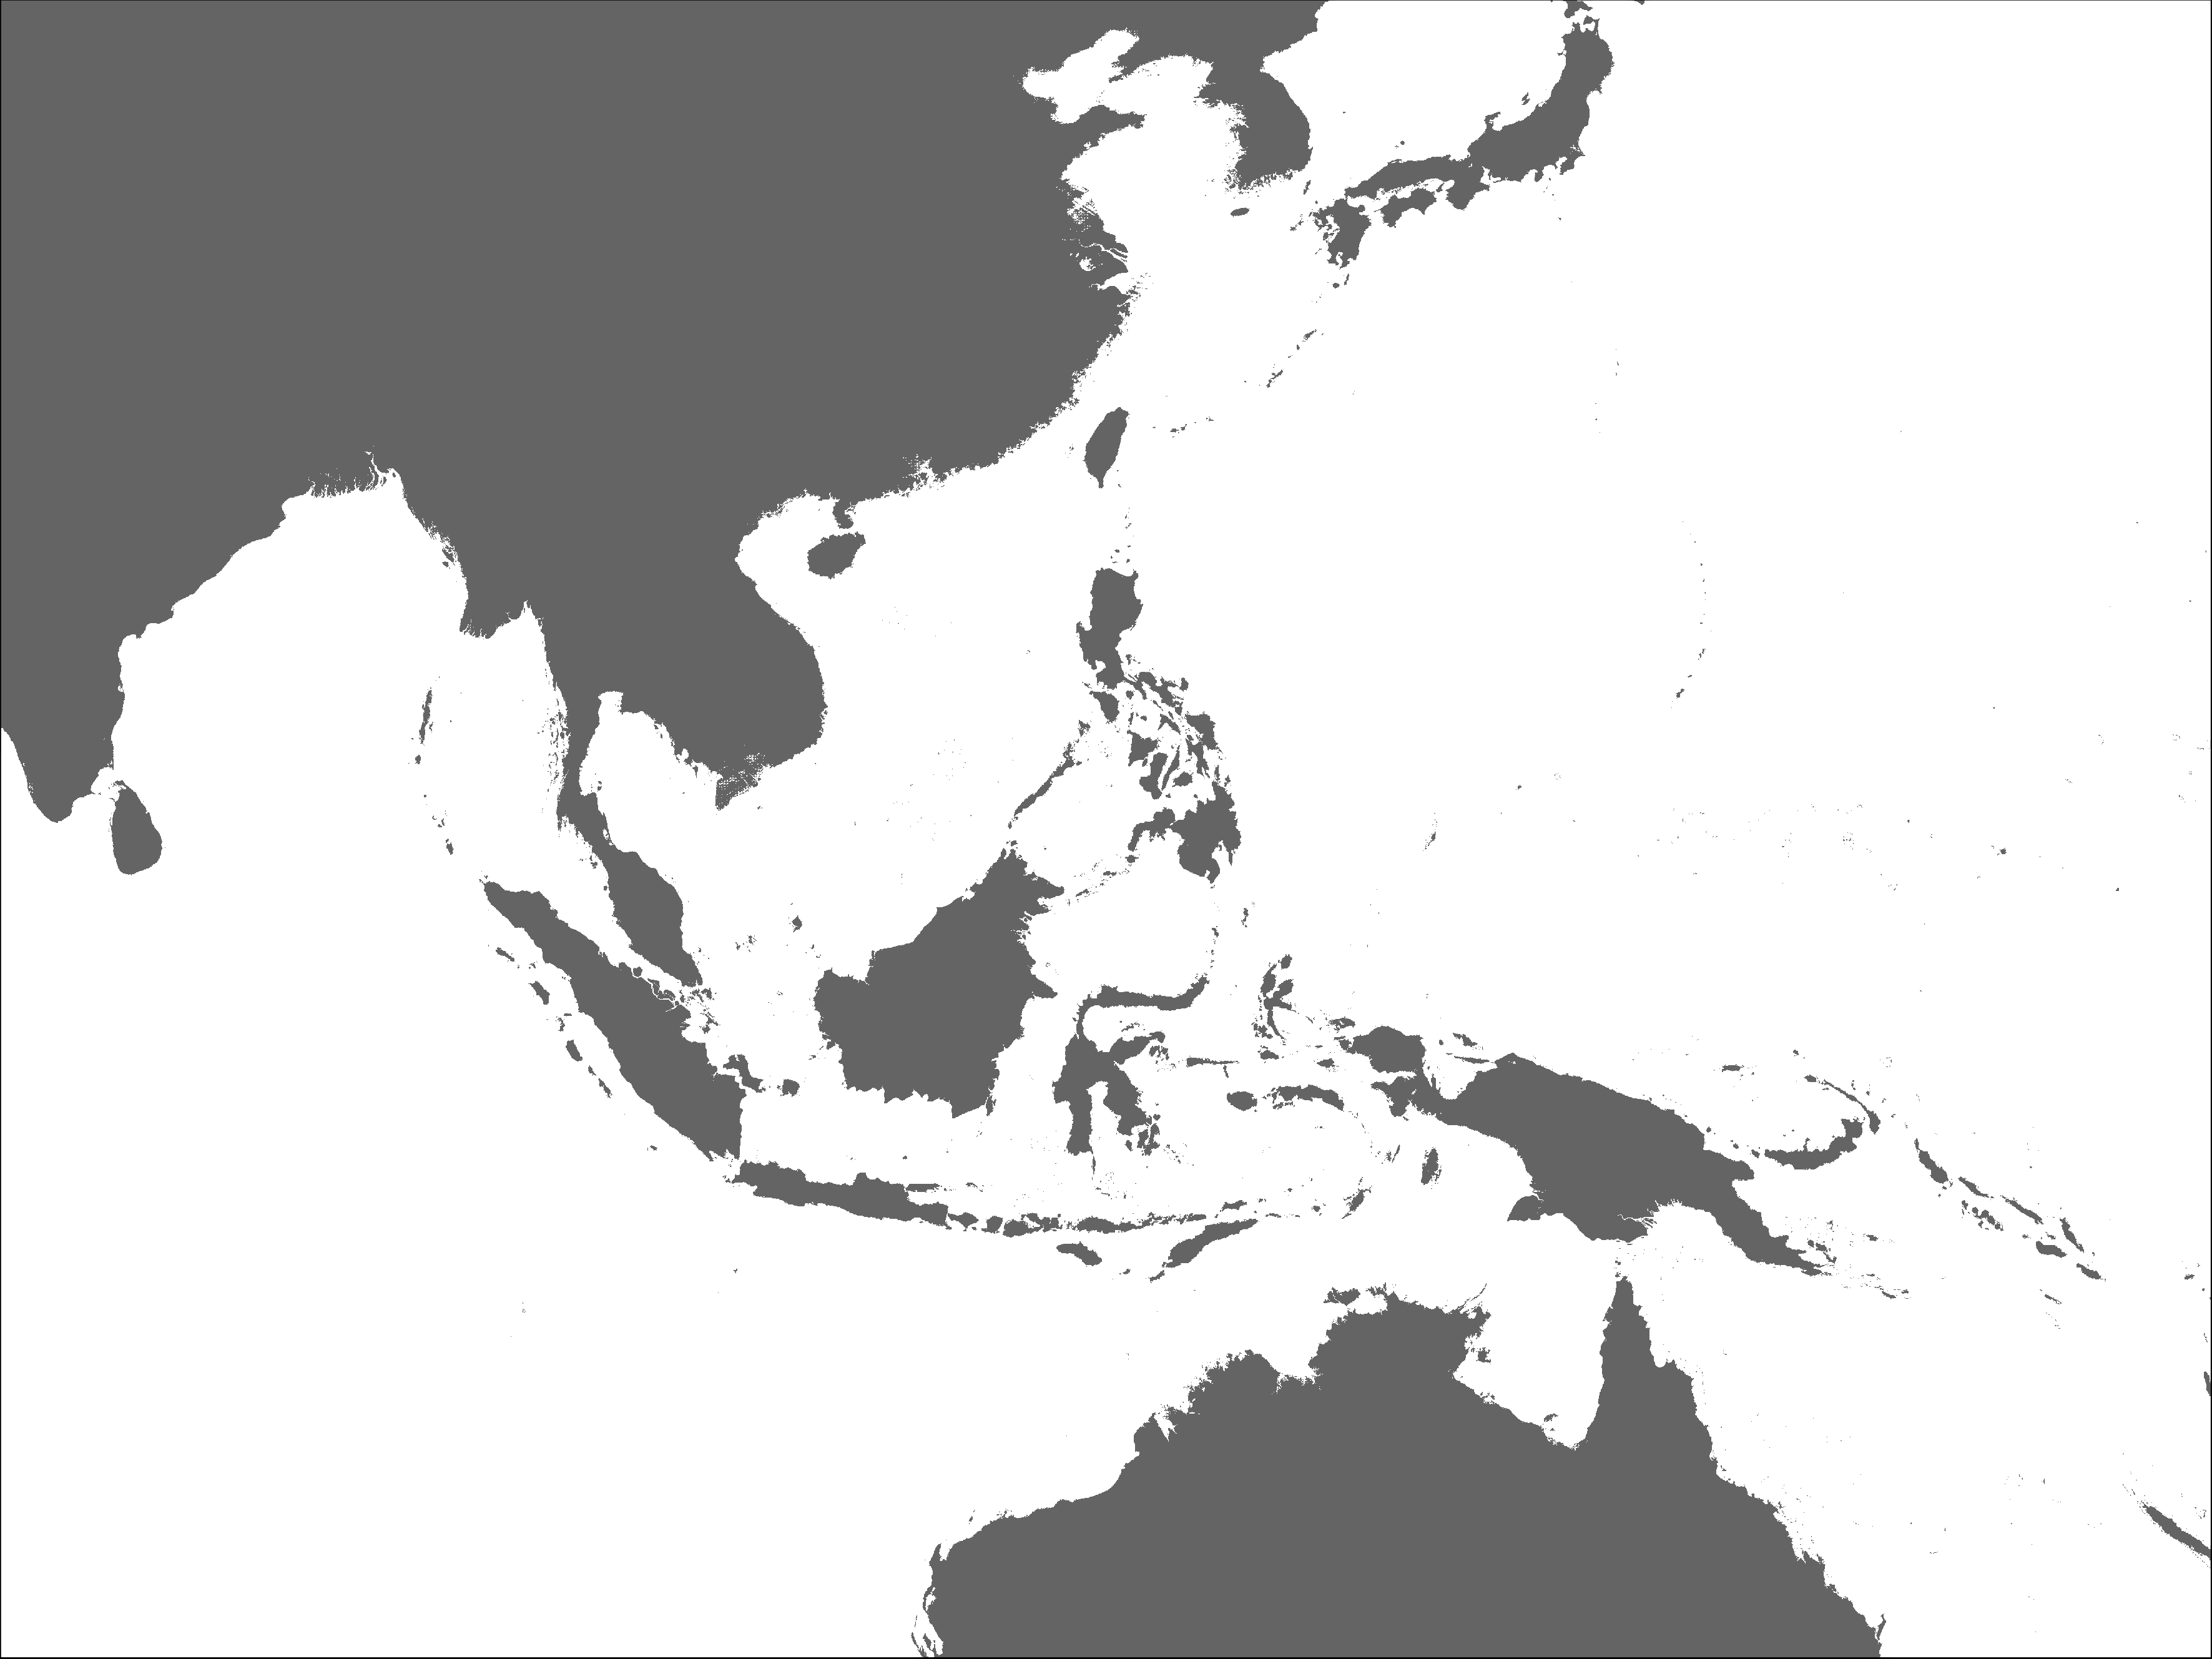
\includegraphics[width=\paperwidth]{images/maps/se-asia-present.png}}
\begin{frame}
    \frametitle{Southeast Asia}    
\end{frame}
}

{
\usebackgroundtemplate{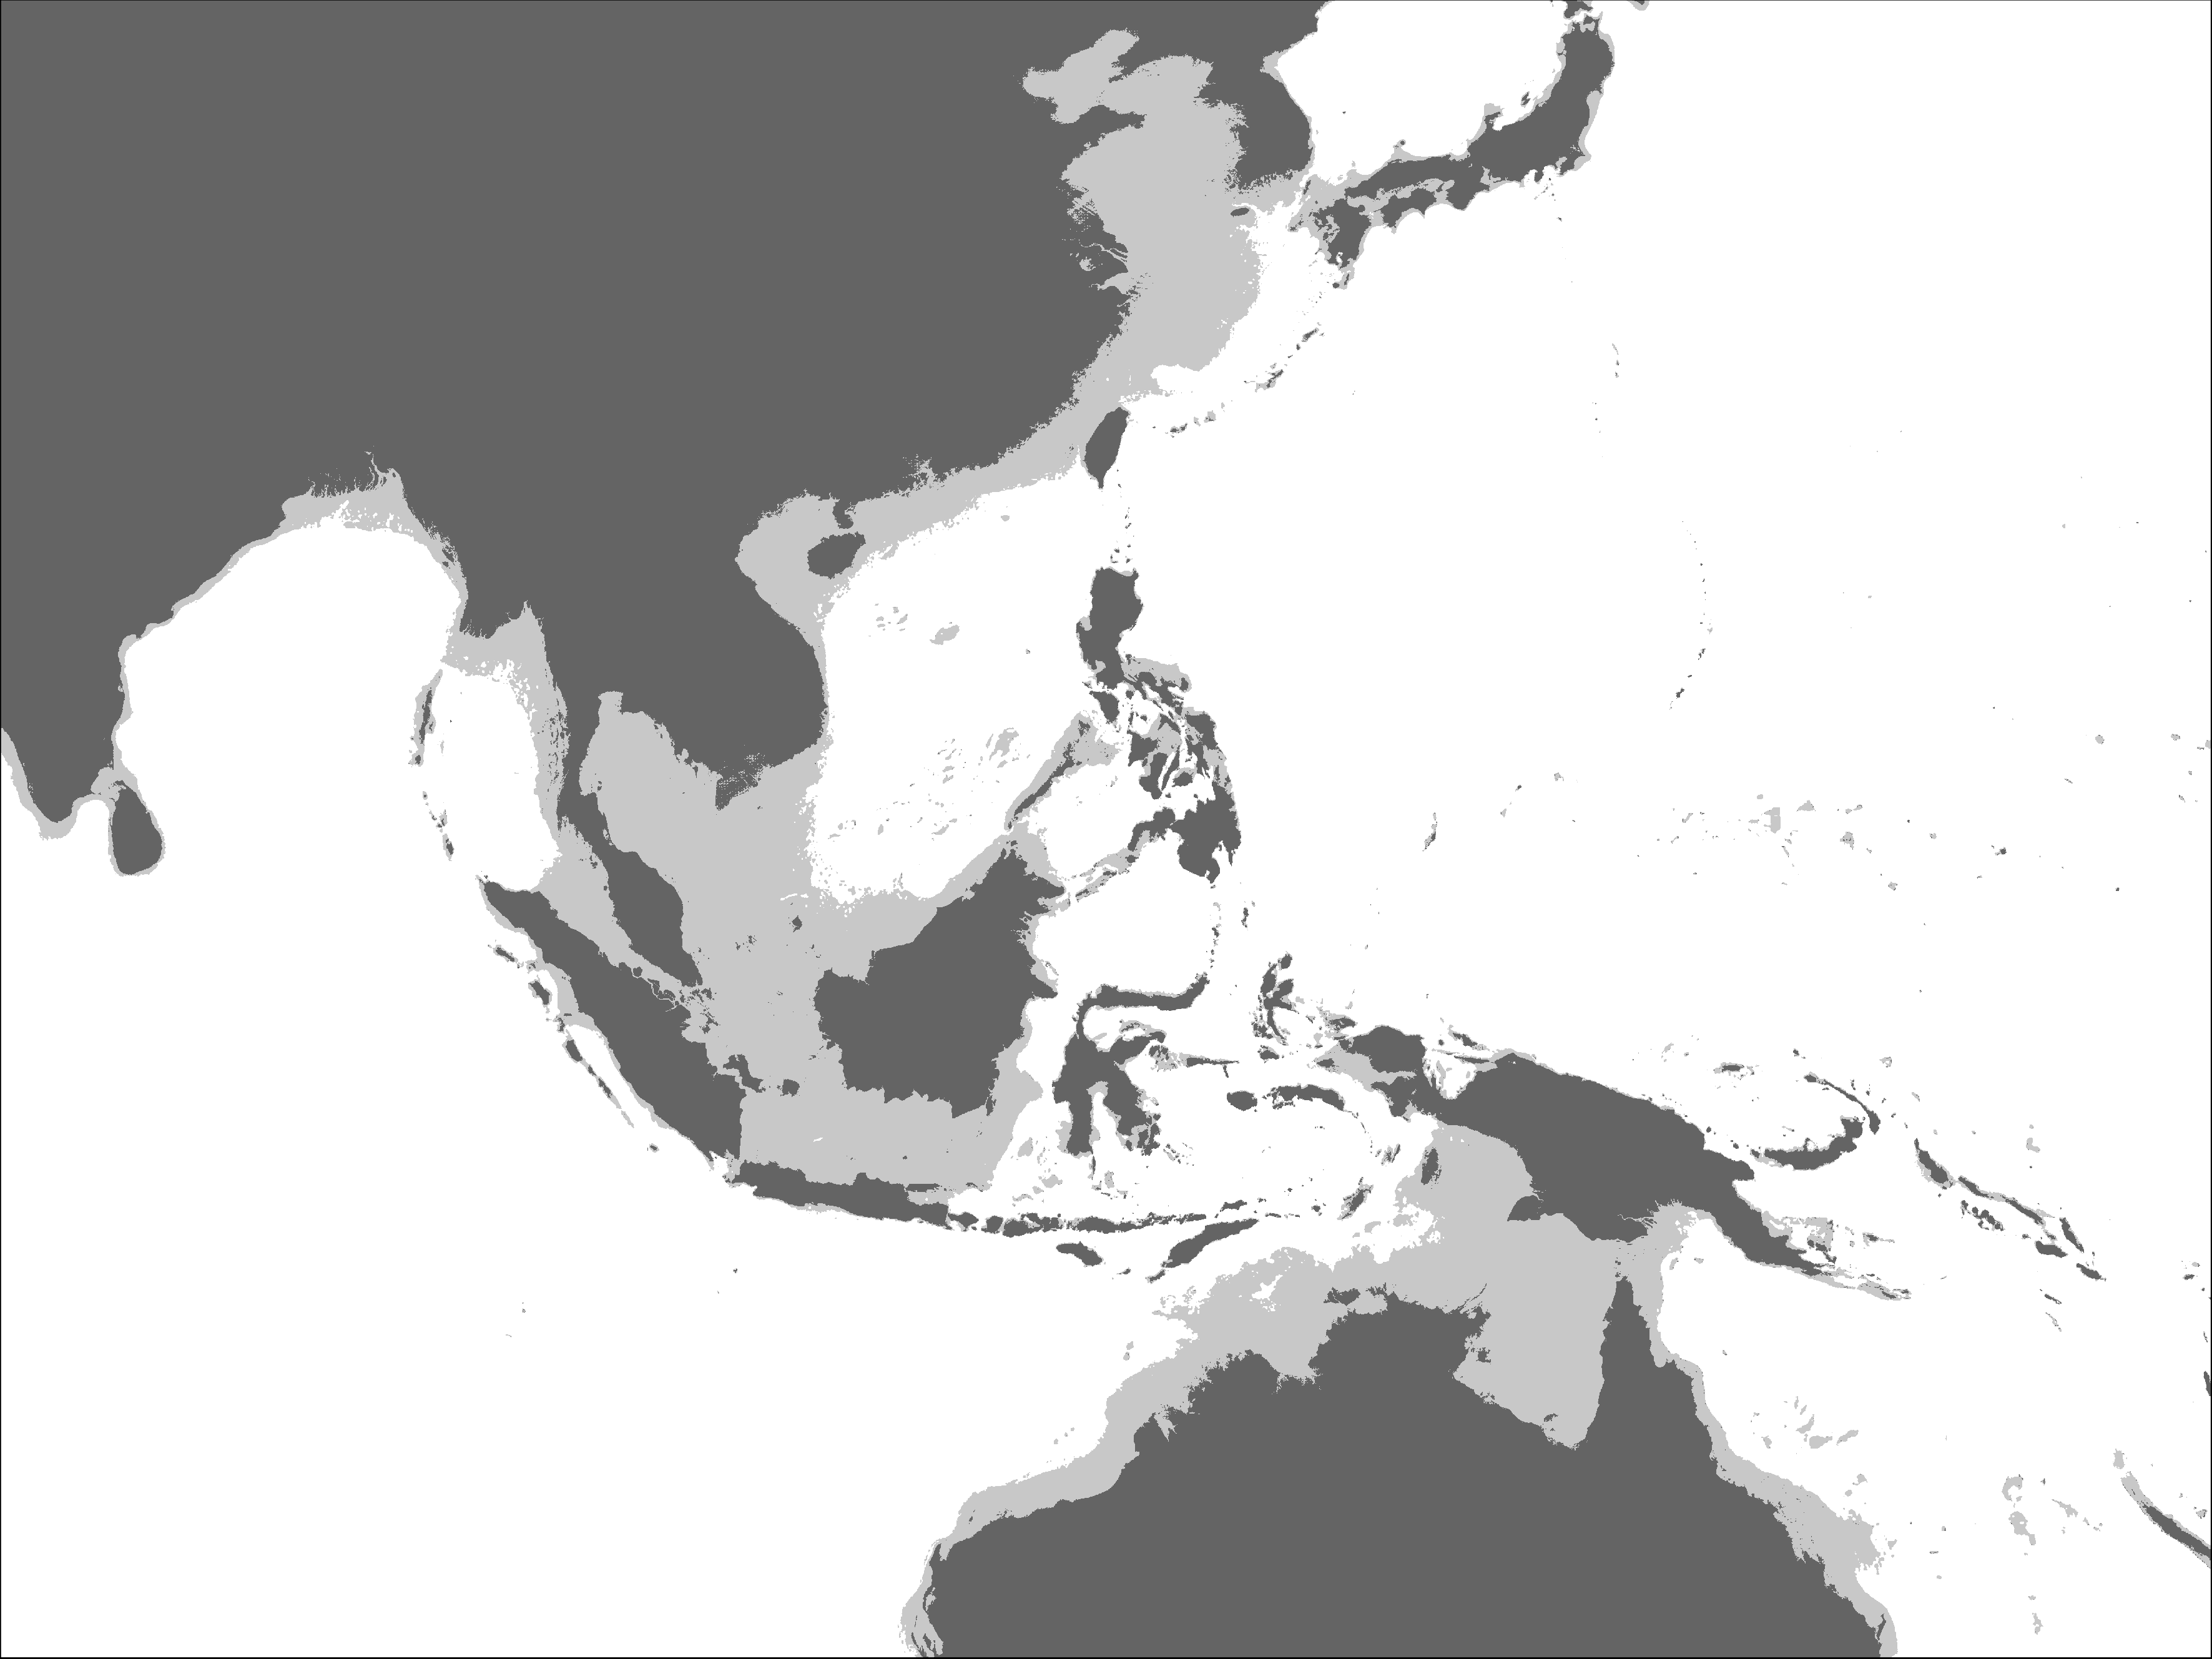
\includegraphics[width=\paperwidth]{images/maps/se-asia-120.png}}
\begin{frame}
    \frametitle{Southeast Asia}    
\end{frame}
}

\subsection{Philippines---Pleistocene model of diversification}

\begin{frame}
    \frametitle{Philippine Archipelago}
    \begin{center}
        \includegraphics<1>[width=.5\textwidth]{images/maps/Philippines-present.png}
        \includegraphics<2>[width=.5\textwidth]{images/maps/Philippines.png}
    \end{center}
\end{frame}

\begin{frame}
    \frametitle{PAIC model}
    \begin{columns}[c]
        \column{.5\textwidth}
            \begin{myitemize}
                \item Repeated coalescence and fragmentation of Pleistocene
                    Aggregate Island Complexes (PAICs)
                \item Prominent paradigm for explaining Philippine biodiversity
                \item Proposed as model of diversification
                % \item Some predictions of the model have been tested
                % \begin{myitemize}
                %     \item Monophyly
                %     \item Does the model explain a large proportion of the diversity?
                % \end{myitemize}
            \end{myitemize}
        \column{.5\textwidth}
            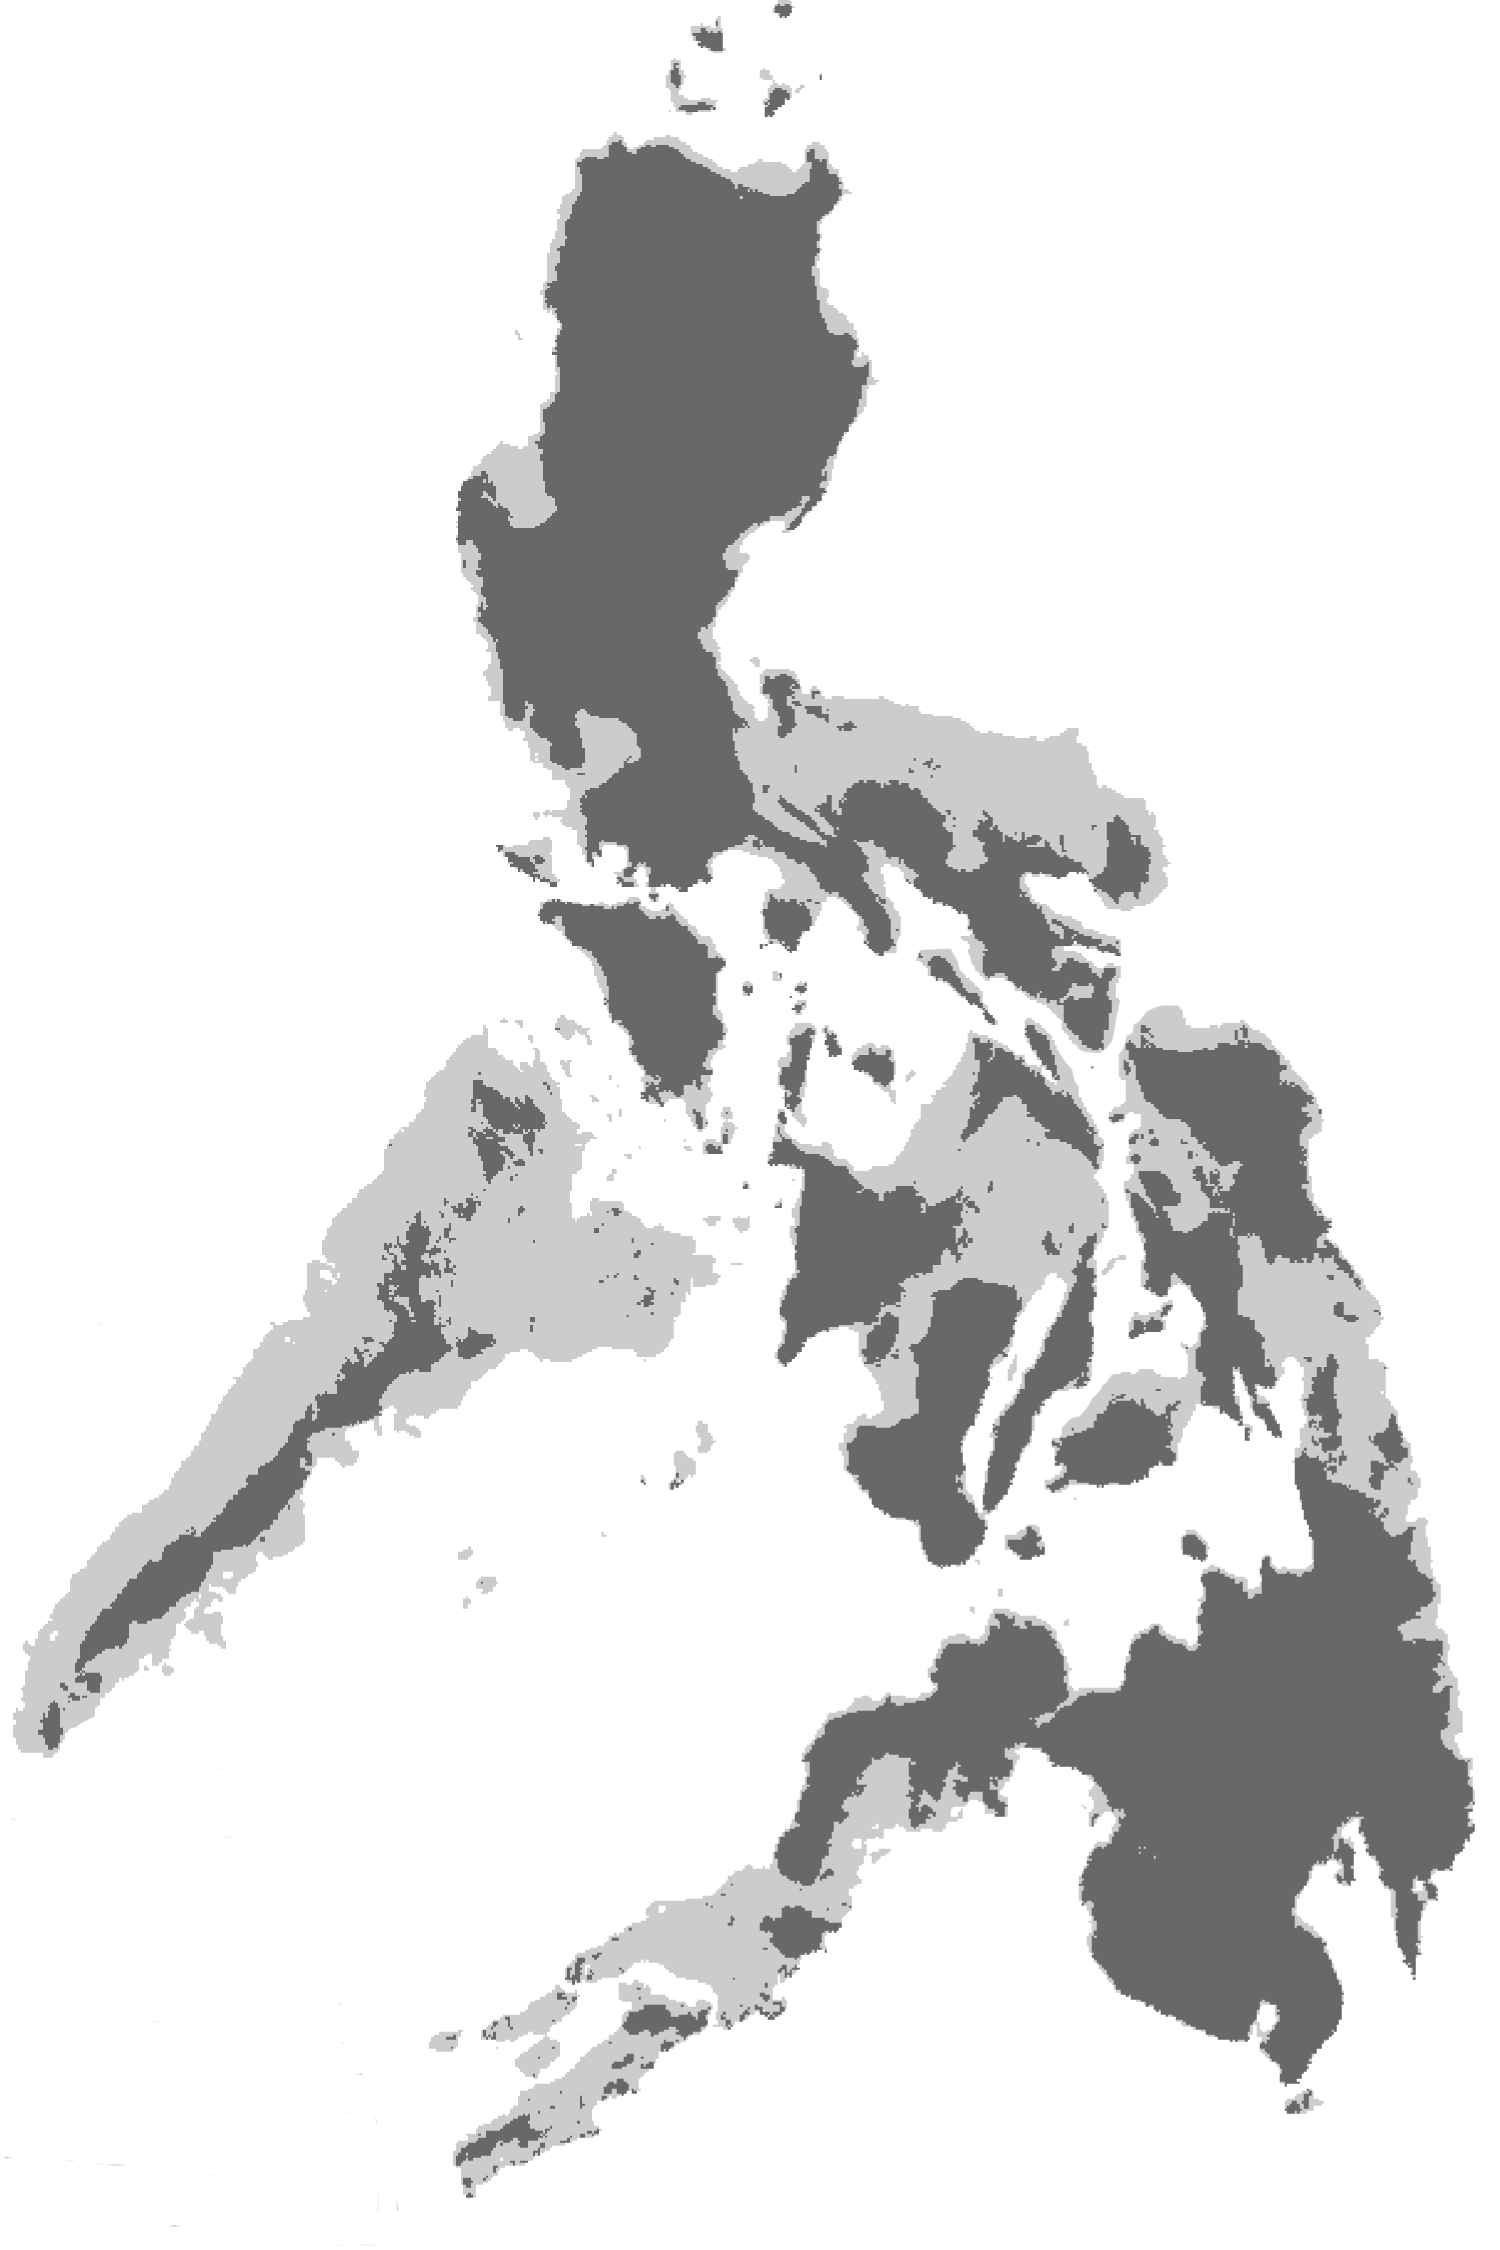
\includegraphics[width=\textwidth]{images/maps/Philippines.png}
    \end{columns}
\end{frame}

\section{Testing the Pleistocene model of diversification}

% \begin{frame}
%     \frametitle{PAIC model: Previous work}
%     \begin{columns}[c]
%         \column{.5\textwidth}
%             \begin{myitemize}
%             \item Phylogenetic work
%                 \begin{myitemize}
%                 \item Are groups of species reciprocally monophyletic among
%                     PAICs?
%                 \item Do most divergences date to the Pleistocene?
%                 \end{myitemize}
%             \item Population genetic work
%                 \begin{myitemize}
%                 \item Are islands within PAICs responsible for most of the
%                     genetic diversity?
%                 \end{myitemize}
%             \end{myitemize}

%             These approaches are really testing the prediction:
%             {\bf The PAIC cycles generated a large proportion of the species
%             diversity in the Philippines.}
%         \column{.5\textwidth}
%             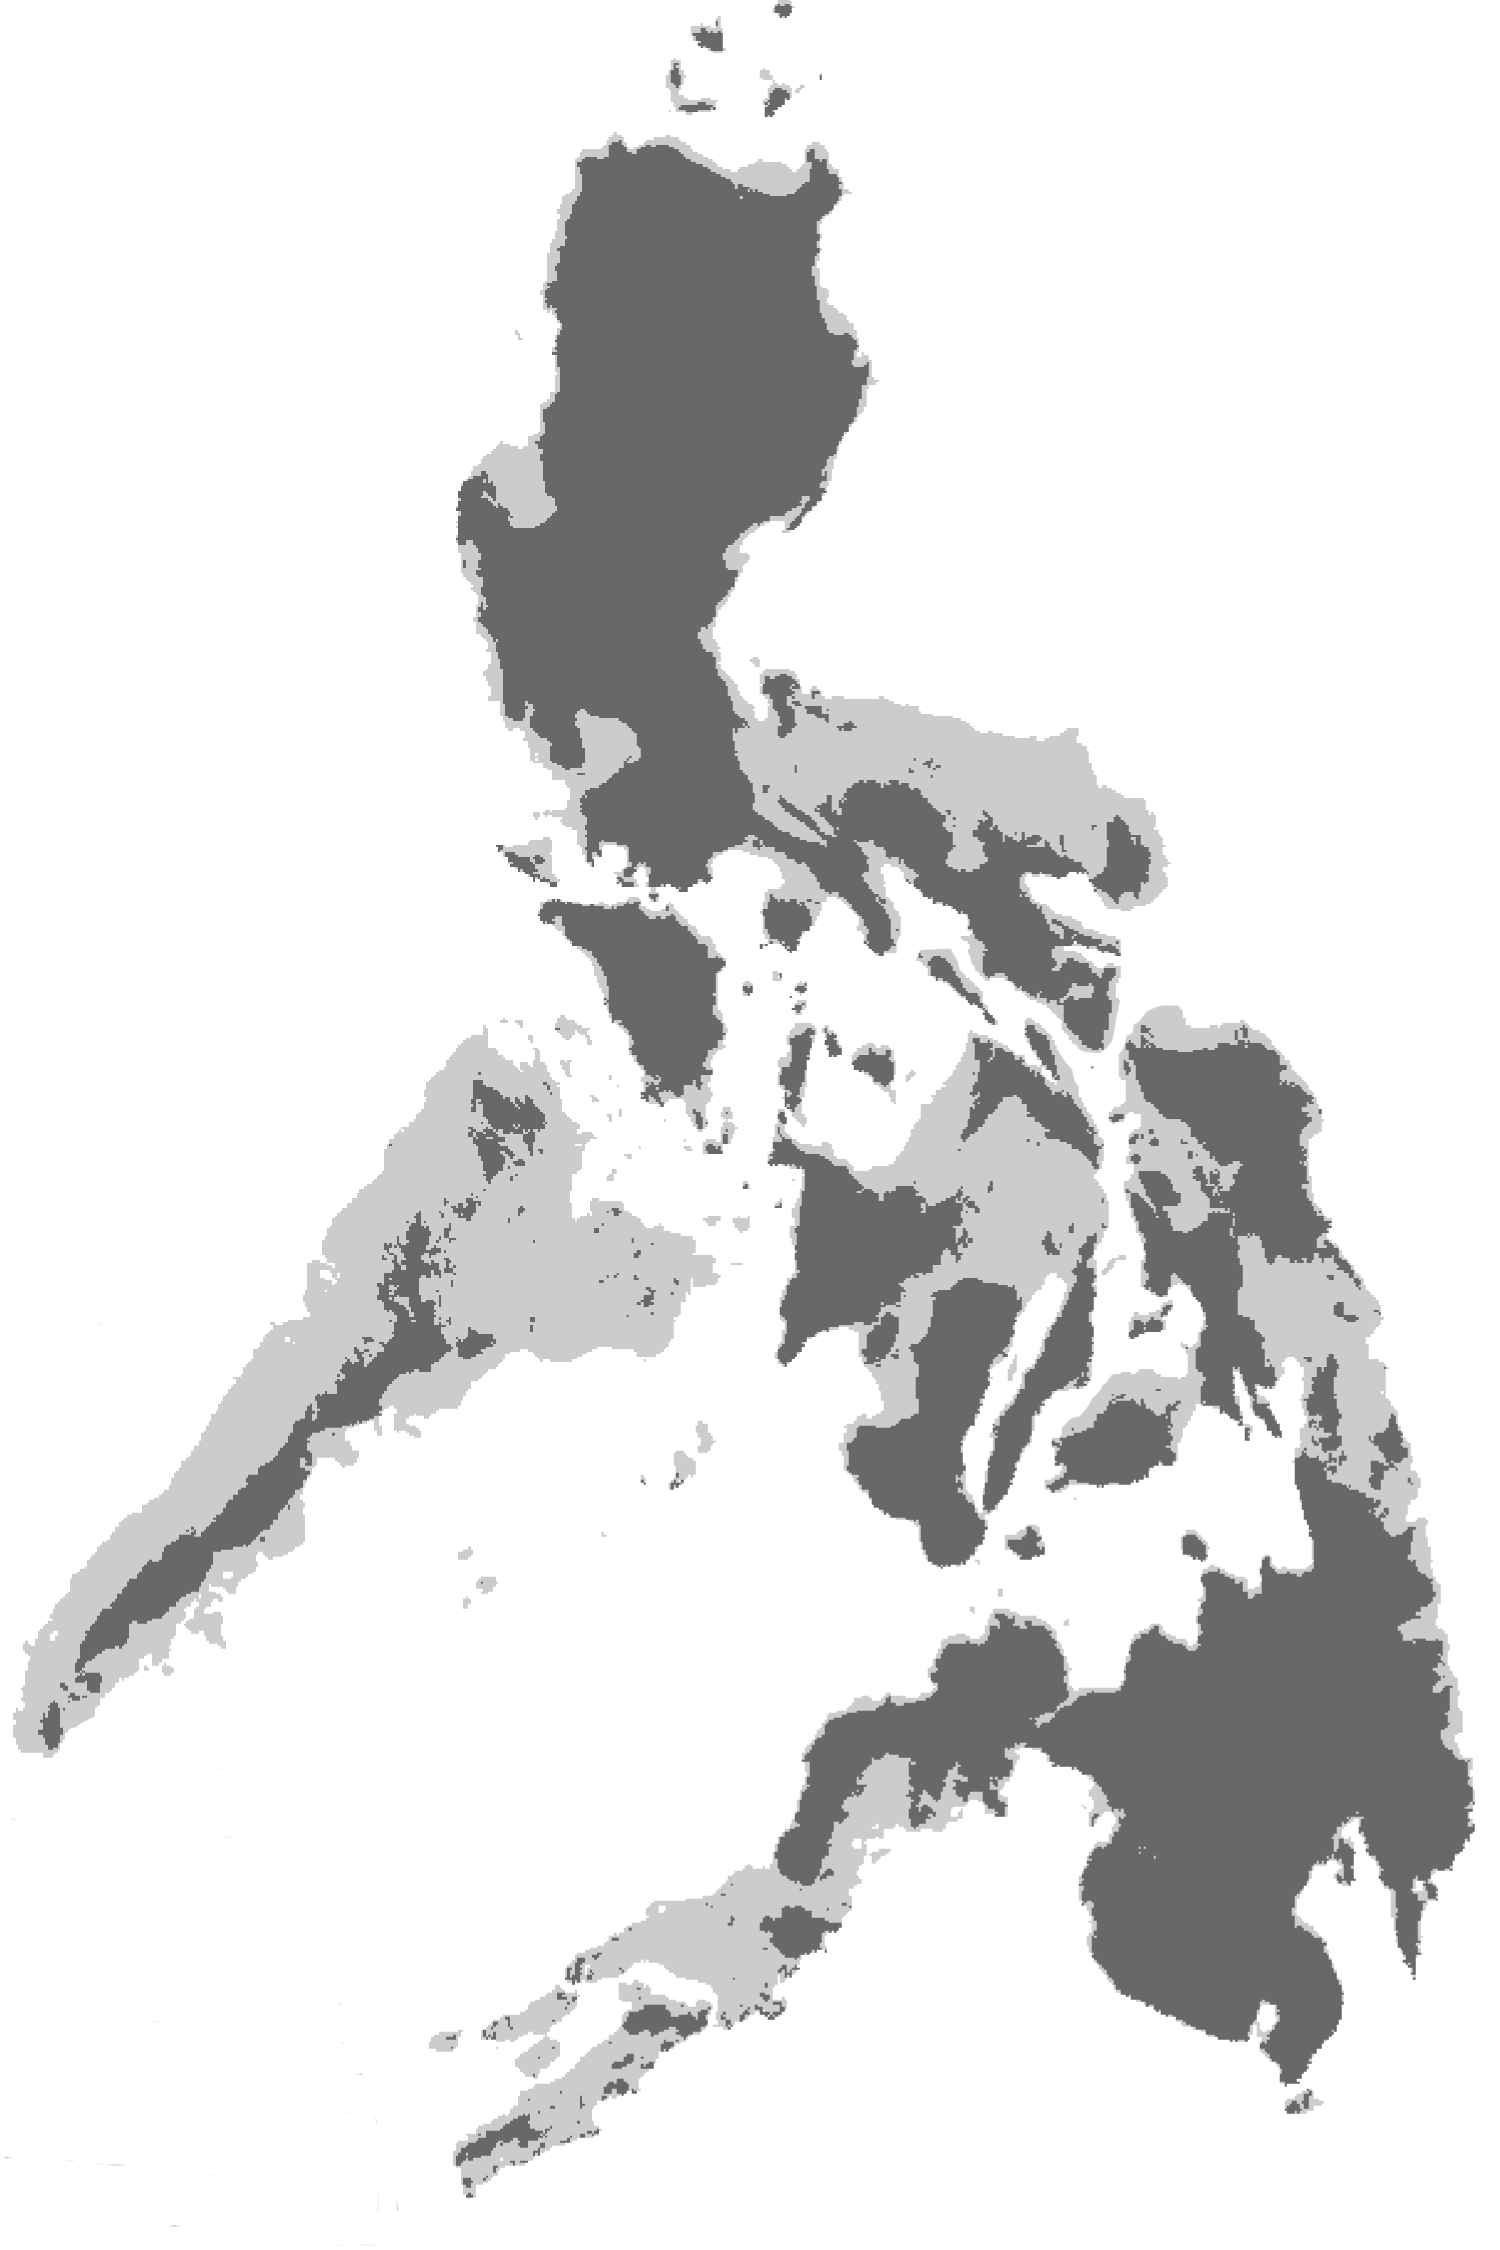
\includegraphics[width=\textwidth]{images/maps/Philippines.png}
%     \end{columns}
% \end{frame}

\begin{frame}
    \frametitle{PAIC model: A new approach}
    % \begin{columns}[c]
    %     \column{.5\textwidth}
            \begin{mydescription}
                \item[$H_0$] Repeated island fragmentation promoted diversification
                    among island populations
                    \begin{mydescription}
                        \item[Prediction] Temporal distribution of divergences
                            between inter-island populations within PAICs
                            should be temporally clustered and correspond with
                            interglacial rises in sea level
                    \end{mydescription}
                \item[$H_1$] Island fragmentation did not promote diversification
                    \begin{mydescription}
                        \item[Prediction] Inter-island diversification was
                            dispersal mediated; no temporal clustering
                    \end{mydescription}
            \end{mydescription}
            
            {\bf Key pattern:} The temporal distribution of divergences
                    among species distributed across PAIC islands
        % \column{.5\textwidth}
        %     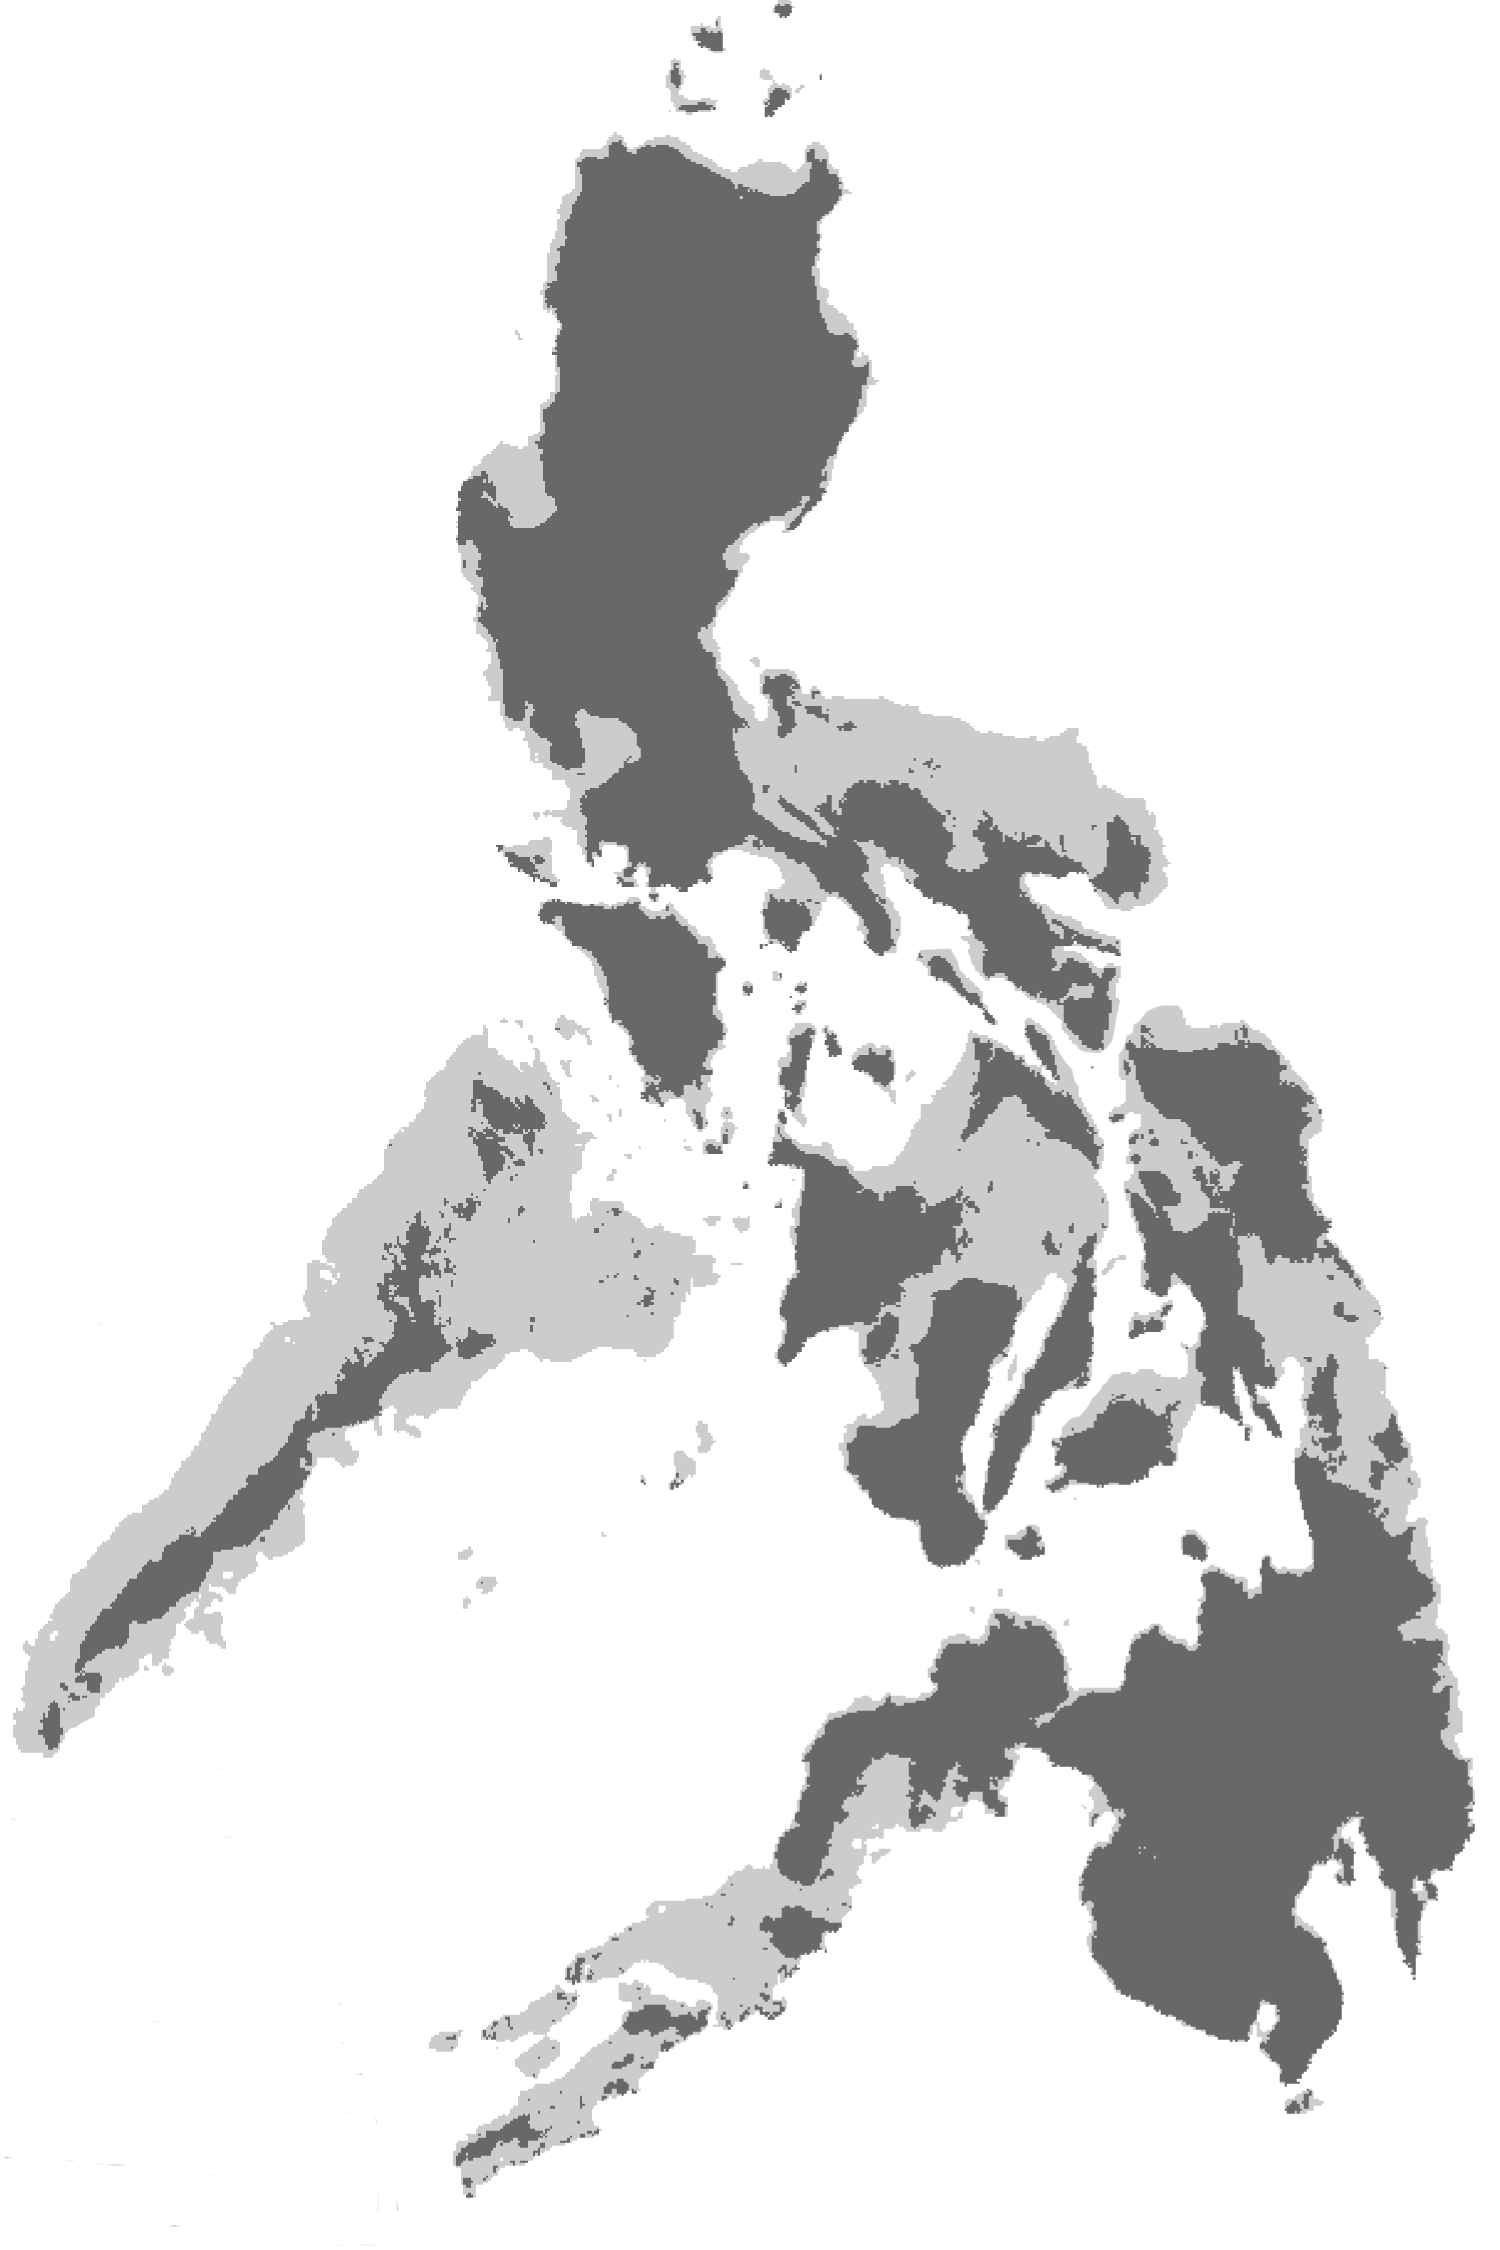
\includegraphics[width=\textwidth]{images/maps/Philippines.png}
    % \end{columns}
\end{frame}

\begin{frame}
    \frametitle{PAIC model: predictions}
    \centerline{
    \includegraphics<1>[width=\textwidth]{images/sea-level-prediction-bare.pdf}
    \includegraphics<2>[width=\textwidth]{images/sea-level-prediction-trees.pdf}
    \includegraphics<3>[width=\textwidth]{images/sea-level-prediction-trees-labels.pdf}
    }
\end{frame}

\begin{frame}
    \frametitle{The method: \msb}
    \begin{columns}[c]
        \column{.4\textwidth}
            \begin{onlyenv}<2>
            \begin{displaybox}[4.5cm]
                \[
                    \divTimeVector = \{\divTime{1},\divTime{2}\}
                \]\vspace{0mm}
                \[
                    \divTimeIndexVector = (\divTimeIndex{1},\divTimeIndex{2},\divTimeIndex{3},\divTimeIndex{4},\divTimeIndex{5})
                \]\vspace{0mm}
                {\small
                \[
                    \divTimeMapVector = (\divTimeMap{1},\divTimeMap{2},\divTimeMap{3},\divTimeMap{4},\divTimeMap{5})
                \]\vspace{0mm}
                }
            \end{displaybox}
            \end{onlyenv}
            \begin{onlyenv}<3>
            \begin{displaybox}[4.5cm]
                \[
                    \divTimeVector = \{125,330\}
                \]\vspace{0mm}
                \[
                    \divTimeIndexVector = (2,2,1,1,1)
                \]\vspace{0mm}
                {\small
                \[
                    \divTimeMapVector = (330,330,125,125,125)
                \]\vspace{0mm}
                }
            \end{displaybox}
            \end{onlyenv}
            \begin{onlyenv}<4>
            \begin{displaybox}[4.5cm]
                \[
                    \divTimeVector = \{125,330\}
                \]\vspace{0mm}
                \[
                    \divTimeIndexVector = (2,2,1,2,1)
                \]\vspace{0mm}
                {\small
                \[
                    \divTimeMapVector = (330,330,125,330,125)
                \]\vspace{0mm}
                }
            \end{displaybox}
            \end{onlyenv}
            \begin{onlyenv}<5>
            \begin{displaybox}[4.5cm]
                {\small
                \vspace{0.7mm}
                \[
                    \divTimeVector = \{125,330,375\}
                \]\vspace{0mm}
                }
                \[
                    \divTimeIndexVector = (3,2,1,2,1)
                \]\vspace{0mm}
                {\small
                \[
                    \divTimeMapVector = (375,330,125,330,125)
                \]\vspace{0mm}
                }
            \end{displaybox}
            \end{onlyenv}
        \column{.6\textwidth}
            \includegraphics<1-3>[height=6.8cm]{images/sea-level-prediction-trees-labels-compact.pdf}
            \includegraphics<4>[height=6.8cm]{images/sea-level-prediction-trees-labels-compact-alt1.pdf}
            \includegraphics<5>[height=6.8cm]{images/sea-level-prediction-trees-labels-compact-alt2.pdf}
    \end{columns}
    
\end{frame}


\subsection{The method---approximate Bayesian model choice}

\begin{frame}
\frametitle{Outline}
\tableofcontents[currentsection,currentsubsection]
\end{frame}

\begin{frame}
    \frametitle{The method: \msb}
        Now we have genetic data for $\npairs{}=22$ taxon pairs, and we need to
        infer the distribution of their relative divergence times
        \[
            \divTimeMapVector = (\divTimeMap{1},\divTimeMap{2},\ldots,\divTimeMap{\npairs{}})
        \]
        where
        \[
            \divTimeVector = \{\divTime{1},\ldots,\divTime{\divTimeNum}\}
        \]
        are the divergence time parameters shared among the taxon pairs, and
        \divTimeNum is the number of divergence time parameters.

        \begin{myitemize}
            \item We want to infer \divTimeMapVector from our data
            \item This is a problem of model choice.
            % \begin{myitemize}
            %     \item Bayesian framework is an attractive approach
            %     \item \msb uses an approximate Bayesian approach to estimate the
            %         posterior probability of competing divergence models
            % \end{myitemize}
        \end{myitemize}
\end{frame}

\begin{frame}
    \frametitle{Bayesian framework}
    Given sequence alignments \alignmentVector and: \\
        \begin{mydescription}
            \item[\divTimeMapVector] The vector of divergence times for each pair of populations
            \item[\geneTreeVector] The gene trees along which the sequences evolved
            \item[\demographicParamVector, \hkyModelVector] The demographic and mutational parameters
        \end{mydescription}
    % \smallskip
    \begin{displaybox}[8.5cm]
    \[
        p(\geneTreeVector, \divTimeMapVector, \demographicParamVector
        \given
        \alignmentVector, \hkyModelVector) =
        \frac{p(\alignmentVector \given \geneTreeVector, \divTimeMapVector,
        \demographicParamVector, \hkyModelVector)
        p(\geneTreeVector, \divTimeMapVector, \demographicParamVector \given \hkyModelVector)}{
        p(\alignmentVector)}
    \]\vspace{0mm}
    \end{displaybox}
    \smallskip
    \[ \alignmentVector \to \ssVectorObs \]
    % \smallskip
    \begin{displaybox}[9.5cm]
    \[
        p(\geneTreeVector, \divTimeMapVector, \demographicParamVector
        \given
        \ssSpace, \hkyModelVector) =
        \frac{p(\alignmentVector \given \geneTreeVector, \divTimeMapVector,
        \demographicParamVector, \hkyModelVector)
        p(\geneTreeVector, \divTimeMapVector, \demographicParamVector \given \hkyModelVector)}{
        p(\ssSpace)}
    \]\vspace{0mm}
    \end{displaybox}

\end{frame}

\begin{frame}[t]
    \frametitle{The \msb model}
    \begin{displaybox}[8.5cm]
    \[
        p(\geneTreeVector, \divTimeMapVector, \demographicParamVector
        \given
        \alignmentVector, \hkyModelVector) =
        \frac{p(\alignmentVector \given \geneTreeVector, \divTimeMapVector,
        \demographicParamVector, \hkyModelVector)
        p(\geneTreeVector, \divTimeMapVector, \demographicParamVector \given \hkyModelVector)}{
        p(\alignmentVector)}
    \]\vspace{0mm}
    \end{displaybox}
    \smallskip
    \begin{onlyenv}<2>
    \begin{block}{\it Full Model:}
    {\tiny
    \begin{equation*}
        \begin{split}
        & p(\geneTreeVector,
        \divTimeMapVector,
        \ancestralThetaVector,
        \descendantThetaVector{1}, \descendantThetaVector{2},
        \bottleTimeVector, \bottleScalarVector{1},
        \bottleScalarVector{2},
        \migrationRateVector,
        \locusRateHetShapeParameter,
        \locusMutationRateScalarVector \given
        \alignmentVector, \hkyModelVector, \ploidyScalarVector,
        \mutationRateScalarConstantVector) \\
        & = \frac{1}{p(\alignmentVector)}
        p(\divTimeMapVector)
        f(\locusRateHetShapeParameter)
        \Bigg[
        \prod_{i=1}^{\npairs{}}
        p(\ancestralTheta{i})
        p(\descendantTheta{1}{i}, \descendantTheta{2}{i})
        p(\bottleTime{i})
        p(\bottleScalar{1}{i}) f(\bottleScalar{2}{i})
        p(\migrationRate{i}) \\
        &
        \prod_{j=1}^{\nloci{i}}
        p(\alignment{i}{j} \given
        \geneTree{i}{j}, \hkyModel{i}{j})
        p(\geneTree{i}{j} \given
        \divTimeMap{i},
        \ancestralTheta{i}, \descendantTheta{1}{i}, \descendantTheta{2}{i},
        \ploidyScalar{i}{j}, \mutationRateScalarConstant{i}{j},
        \locusMutationRateScalar{j},
        \bottleTime{i}, \bottleScalar{1}{i}, \bottleScalar{2}{i},
        \migrationRate{i})
        \Bigg]
        \Bigg[
        \prod_{j=1}^{\nlociTotal}
        f(\locusMutationRateScalar{j} \given \locusRateHetShapeParameter)
        \Bigg]
        \label{eq:fullmodel}
        \end{split}
    \end{equation*}
    }
    \end{block}
    \end{onlyenv}
    \only<3>{
        \begin{mydescription}
            \item[\divTimeMapVector] The vector of divergence times for each pair of populations
            \item[\divTimeNum] The number of unique divergence times within \divTimeMapVector
            \item[\divTimeDispersion] The variance of \divTimeMapVector
        \end{mydescription}
        \vspace{1cm}
    }
\end{frame}

\subsection{The data}

% \begin{frame}
% \frametitle{Outline}
% \tableofcontents[currentsection,currentsubsection]
% \end{frame}

\begin{frame}
\begin{columns}[c]
    \column{.5\textwidth}
        \begin{table}%[htbp]
            \scriptsize
            \addtolength{\tabcolsep}{-0.09cm}
            \centering
            \begin{tabular}{ l c c }
                % \toprule
                \textbf{Species} & {\boldmath $n_1$} & {\boldmath $n_2$} \\
                \hline
                \textbf{\textsc{Mammals}} & & \\
                \emph{Crocidura beatus}             & 12 & 11 \\
                \emph{Crocidura negrina-panayensis} & 12 & 6  \\
                \emph{Hipposideros obscurus}        & 19 & 9  \\
                \emph{Hipposideros pygmaeus}        & 3  & 12 \\
                \emph{Cynopterus brachyotis}        & 20 & 8  \\
                \emph{Cynopterus brachyotis}        & 8  & 14 \\
                \emph{Haplonycteris fischeri}       & 29 & 8  \\
                \emph{Haplonycteris fischeri}       & 9  & 21 \\
                \emph{Macroglossus minimus}         & 19 & 4  \\
                \emph{Macroglossus minimus}         & 8  & 10 \\
                \emph{Ptenochirus jagori}           & 4  & 7  \\
                \emph{Ptenochirus jagori}           & 8  & 8  \\
                \emph{Ptenochirus minor}            & 30 & 9  \\
                \textbf{\textsc{Squamates}} & & \\
                \emph{Cyrtodactylus gubaot-sumuroi} & 29 & 6  \\
                \emph{Cyrtodactylus annulatus}      & 14 & 3  \\
                \emph{Cyrtodactylus philippinicus}  & 6  & 14 \\
                \emph{Gekko mindorensis}            & 8  & 11 \\
                \emph{Insulasaurus arborens}        & 22 & 10 \\
                \emph{Pinoyscincus jagori}          & 8  & 8  \\
                \emph{Dendrelaphis marenae}         & 6  & 6  \\
                \textbf{\textsc{Anurans}}  & & \\
                \emph{Limnonectes leytensis}        & 4  & 2  \\
                \emph{Limnonectes magnus}           & 2  & 3  \\
                \hline
            \end{tabular}
        \end{table}
    \column{.5\textwidth}
        \centerline{
        \includegraphics<1>[height=1.5cm]{images/photos/crocidura-negrina-JAEsselstyn.jpg}}
        % \vspace{0.5mm}
        \centerline{
        \includegraphics<1>[height=1.5cm]{images/photos/hipposideros-obscurus-MRMDuya.jpg}
        \hspace{0.3mm}
        \includegraphics<1>[height=1.5cm]{images/photos/haplonycteris-fischeri-JHolden.jpg}}
        % \vspace{0.5mm}
        \centerline{
        \includegraphics<1>[height=1.5cm]{images/photos/gekko-mindorensis.jpg}
        \hspace{0.3mm}
        \includegraphics<1>[height=1.5cm]{images/photos/sphenomorphus-arborens-rmb.jpg}}
        % \vspace{0.5mm}
        \centerline{
        \includegraphics<1>[height=1.5cm]{images/photos/dendrelaphis-pictus-cds.jpg}}
        % \vspace{0.5mm}
        \centerline{
        \includegraphics<1>[height=1.5cm]{images/photos/limnonectes-leytensis-rmb.jpg}}
\end{columns}
\end{frame}

\begin{frame}
\begin{columns}[c]
    \column{.5\textwidth}
        \begin{table}%[htbp]
            \scriptsize
            \addtolength{\tabcolsep}{-0.09cm}
            \def\firstrowcolor{}
            \def\secondrowcolor{}
            \def\thirdrowcolor{}
            \def\fourthrowcolor{}
            \def\fifthrowcolor{}
            \only<2>{\def\firstrowcolor{\rowcolor{rowred}}}
            \only<3>{\def\secondrowcolor{\rowcolor{rowred}}}
            \only<4>{\def\thirdrowcolor{\rowcolor{rowred}}}
            \only<5>{\def\fourthrowcolor{\rowcolor{rowred}}}
            \only<6>{\def\fifthrowcolor{\rowcolor{rowred}}}
            \centering
            \begin{tabular}{ l c c }
                % \toprule
                \textbf{Species} & {\boldmath $n_1$} & {\boldmath $n_2$} \\
                \hline
                \textbf{\textsc{Mammals}} & & \\
                \fifthrowcolor  \emph{Crocidura beatus}             & 12 & 11 \\
                \firstrowcolor  \emph{Crocidura negrina-panayensis} & 12 & 6  \\
                \thirdrowcolor  \emph{Hipposideros obscurus}        & 19 & 9  \\
                \secondrowcolor \emph{Hipposideros pygmaeus}        & 3  & 12 \\
                \thirdrowcolor  \emph{Cynopterus brachyotis}        & 20 & 8  \\
                \firstrowcolor  \emph{Cynopterus brachyotis}        & 8  & 14 \\
                \thirdrowcolor  \emph{Haplonycteris fischeri}       & 29 & 8  \\
                \firstrowcolor  \emph{Haplonycteris fischeri}       & 9  & 21 \\
                \thirdrowcolor  \emph{Macroglossus minimus}         & 19 & 4  \\
                \firstrowcolor  \emph{Macroglossus minimus}         & 8  & 10 \\
                \thirdrowcolor  \emph{Ptenochirus jagori}           & 4  & 7  \\
                \firstrowcolor  \emph{Ptenochirus jagori}           & 8  & 8  \\
                \thirdrowcolor  \emph{Ptenochirus minor}            & 30 & 9  \\
                \textbf{\textsc{Squamates}} & & \\
                \fifthrowcolor  \emph{Cyrtodactylus gubaot-sumuroi} & 29 & 6  \\
                \secondrowcolor \emph{Cyrtodactylus annulatus}      & 14 & 3  \\
                \firstrowcolor  \emph{Cyrtodactylus philippinicus}  & 6  & 14 \\
                \firstrowcolor  \emph{Gekko mindorensis}            & 8  & 11 \\
                \firstrowcolor  \emph{Insulasaurus arborens}        & 22 & 10 \\
                \fourthrowcolor \emph{Pinoyscincus jagori}          & 8  & 8  \\
                \firstrowcolor  \emph{Dendrelaphis marenae}         & 6  & 6  \\
                \textbf{\textsc{Anurans}}  & & \\
                \secondrowcolor \emph{Limnonectes leytensis}        & 4  & 2  \\
                \secondrowcolor \emph{Limnonectes magnus}           & 2  & 3  \\
                \hline
            \end{tabular}
        \end{table}
    \column{.5\textwidth}
        \includegraphics<1>[width=\textwidth]{images/maps/Philippines.png}
        \includegraphics<2>[width=\textwidth]{images/maps/Philippines-negros_panay.png}
        \includegraphics<3>[width=\textwidth]{images/maps/Philippines-bohol_mindanao.png}
        \includegraphics<4>[width=\textwidth]{images/maps/Philippines-leyte_mindanao.png}
        \includegraphics<5>[width=\textwidth]{images/maps/Philippines-mindanao_samar.png}
        \includegraphics<6>[width=\textwidth]{images/maps/Philippines-leyte_samar.png}
\end{columns}
\end{frame}


\section{Empirical results}
\subsection{Too good to be true?}

\begin{frame}
\frametitle{Outline}
\tableofcontents[currentsection,currentsubsection]
\end{frame}

\begin{frame}
    \frametitle{Empirical results}
    \begin{columns}[c]
        \column{.4\textwidth}
            {\small
            Strong support for simultaneous divergence of all 22 taxon pairs \\
            \vspace{1cm}
            pp $>$ 0.96 \\
            \vspace{1cm}
            $\sim$100,000--250,000 years ago}
        \column{.6\textwidth}
        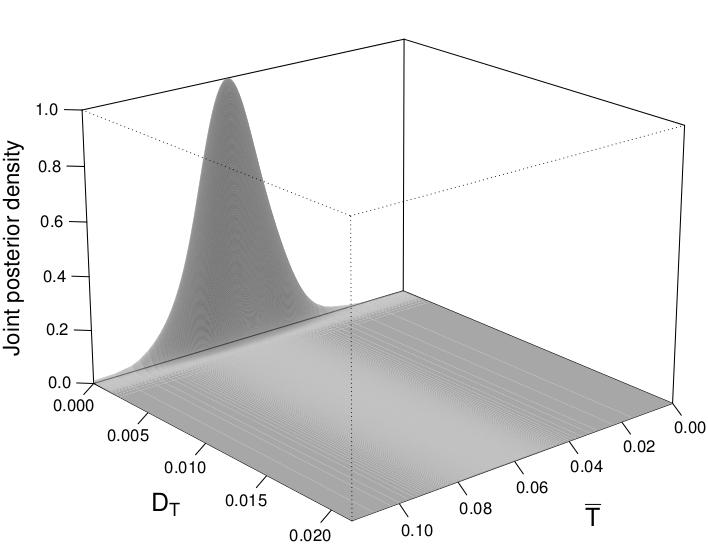
\includegraphics[width=\textwidth]{images/jointDensityPlotsSlide.jpg}
    \end{columns}
\end{frame}

\section{Simulation-based assessment of method}

\begin{frame}
\frametitle{Outline}
\tableofcontents[currentsection,currentsubsection]
\end{frame}

\begin{frame}
    \frametitle{Simulation-based power analyses}
    What is ``simultaneous''?
    \begin{myitemize}
        \item Draw divergence times from $U(0, \divt{max})$
        \item \divt{max} was set to:
            0.1, 0.2, 0.3, 0.4, 0.5, 0.6, 0.7, 0.8, 0.9, 1.0, 2.0, and 3.0
        \item Units are \globalcoalunit generations
    \end{myitemize}
\end{frame}

\begin{frame}[t]
    \frametitle{Simulation results: Power}
    \vspace{1cm}
        \centerline{
        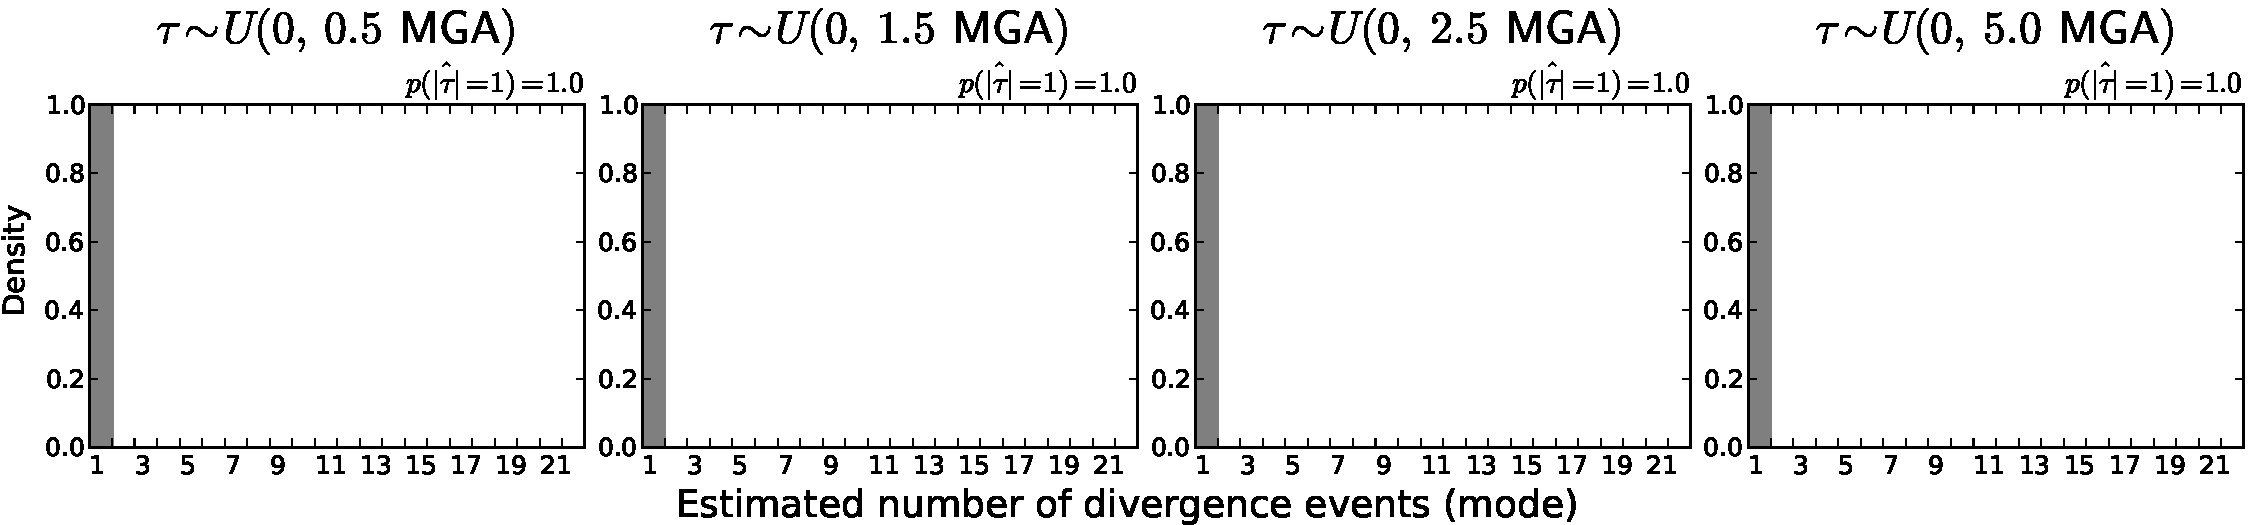
\includegraphics[width=\textwidth]{images/old-sims_power_psi_mode.pdf}}
        \vspace{0mm}
        \centerline{
        \includegraphics<2>[width=\textwidth]{images/old-sims_power_psi_prob_headless.pdf}}
\end{frame}

\begin{frame}
    \frametitle{Simulation results: Summary}
    Estimates of highly clustered divergences when divergence times are random
    over the past 7.5 million generations \\
    \bigskip
    More than 5\% of replicates estimate strong support (BF $>$ 10) for
    extreme case of one divergence when divergences are random over past 3
    million generations \\
    \bigskip
    More than 5\% of replicates estimate extreme case of one divergence based
    on \vmratio{} when divergences are random over past 2 million generations
\end{frame}

\subsection{Why the odd behavior?}

\begin{frame}
\frametitle{Outline}
\tableofcontents[currentsection,currentsubsection]
\end{frame}

\begin{frame}
    \frametitle{Causes of bias}
    Potential causes of the bias:
    \begin{enumerate}
        \item The prior on divergence models
        \item Broad uniform priors on many of the model's parameters, including
            divergence times
            \begin{enumerate}
                \item Small marginal likelihoods of rich models
                \item Insufficient sampling of rich models
            \end{enumerate}
        \item Theoretical limitations of ABC model choice
    \end{enumerate}
\end{frame}

\begin{frame}
    \frametitle{Causes of bias: Prior on divergence models}
    \begin{itemize}
        \item \msb uses a discrete uniform prior on the \emph{number} of
            divergence events, \divTimeNum
    % \vspace{0.1cm}
        \item Each class of \divTimeNum represents a different number of
            divergence models, i.e., the number of integer partitions
            \divTimeNum into \npairs{}
    % \vspace{0.1cm}
        \item This creates a U-shaped prior on divergence models that disfavors
            models with intermediate numbers of events
    \end{itemize}
    % \smallskip
    \centerline{
    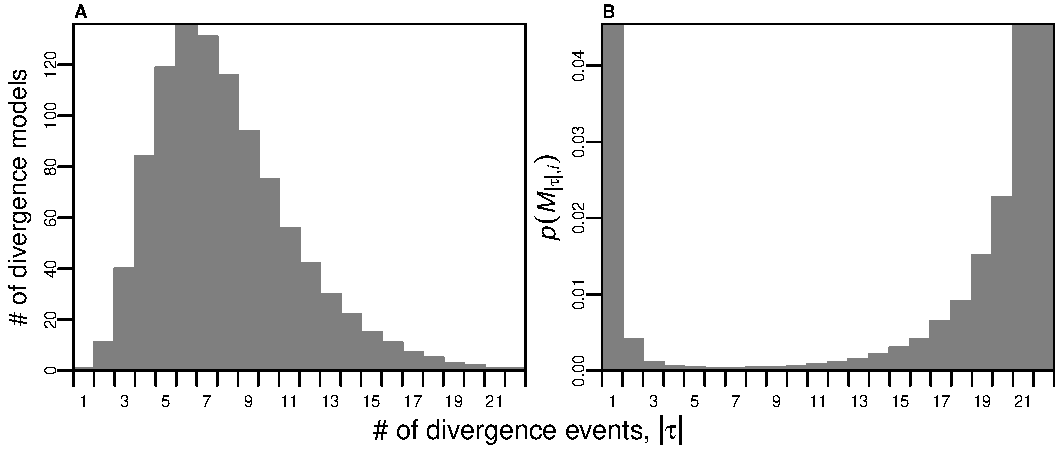
\includegraphics[width=\textwidth]{images/partition_numbers.pdf}}
\end{frame}


\begin{frame}
    \frametitle{Causes of bias: Priors on nuisance parameters}
    % \begin{displaybox}[5.5cm]
    %     \small
    %     \[
    %         p(X) = \int_{\theta} p(X
    %         \given \theta) p(\theta) \mathrm{d}\theta
    %     \]%\vspace{0mm}
    % \end{displaybox}
    \begin{itemize}
        \item \msb uses uniform priors on most model parameters, including
            divergence times
        \item This requires the use of broad priors
        \item Models with more divergence-time parameters have much greater
            parameter space, much of it with low likelihood
        \item This vast space can cause numerical and theoretical problems
        \begin{enumerate}
            \item Insufficient sampling
            \item Reduced marginal likelihoods
        \end{enumerate}
    \end{itemize}
\end{frame}

\begin{frame}
    \frametitle{Causes of bias: Insufficient sampling}
    \begin{itemize}
        \item Models with more parameter space are less densely sampled
        \item Could explain bias toward small models in extreme cases
        \item {\bf Predicts large variance in posterior estimates}
        \begin{itemize}
            \item We explored empirical and simulation-based analyses with
                2, 5, and 10 million prior samples, and estimates were
                very similar
        \end{itemize}
    \end{itemize}
    \smallskip
    \centerline{
    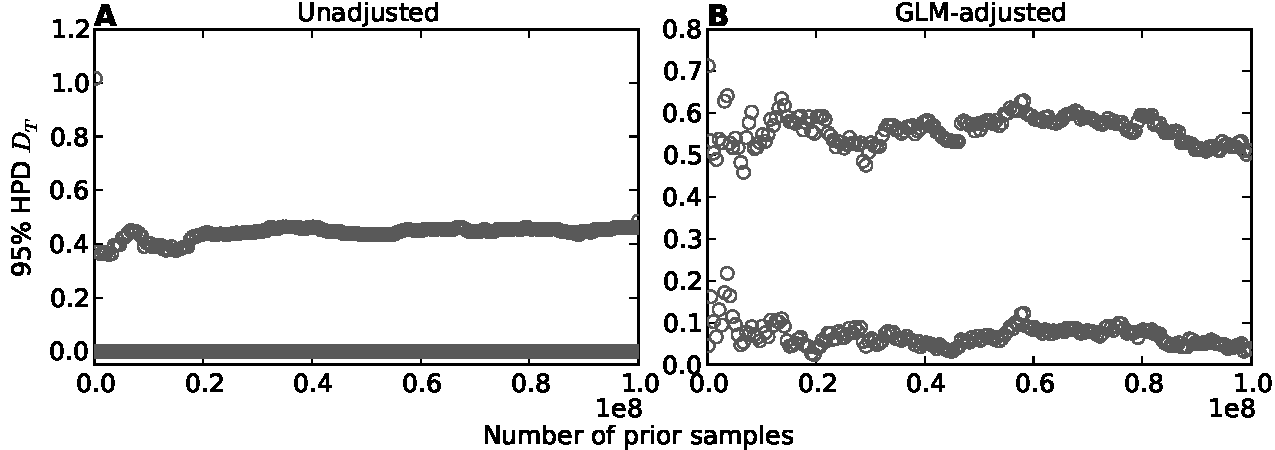
\includegraphics[width=\textwidth]{images/omega_over_sampling.pdf}}
\end{frame}

\begin{frame}
    \frametitle{Causes of bias: Priors on nuisance parameters}
    % \begin{displaybox}[5.5cm]
    %     \small
    %     \[
    %         p(X) = \int_{\theta} p(X
    %         \given \theta) p(\theta) \mathrm{d}\theta
    %     \]%\vspace{0mm}
    % \end{displaybox}
    \begin{itemize}
        \item \msb uses uniform priors on most model parameters, including
            divergence times
        \item This requires the use of broad priors
        \item Models with more divergence-time parameters have much greater
            parameter space, much of it with low likelihood
        \item This vast space can cause numerical and theoretical problems
        \begin{enumerate}
            \item Insufficient sampling
            \item Reduced marginal likelihoods
        \end{enumerate}
    \end{itemize}
\end{frame}

\begin{frame}[t]
    \frametitle{Causes of bias: Marginal likelihoods}
    \begin{displaybox}[5.5cm]
        \small
        \[
            p(X) = \int_{\theta} p(X
            \given \theta) p(\theta) \mathrm{d}\theta
        \]%\vspace{0mm}
    \end{displaybox}
    \smallskip
    \centerline{
        \includegraphics<2>[height=6.5cm]{images/marginal-plot-2d-no-priors.pdf}
        \includegraphics<3>[height=6.5cm]{images/marginal-plot-2d-uniform-prior.pdf}
        % \includegraphics<3>[height=6.5cm]{images/marginal-plot-2d.pdf}
    }
\end{frame}

\begin{frame}
    \frametitle{Causes of bias: Marginal likelihoods}
    % \begin{displaybox}[5.5cm]
    %     \small
    %     \[
    %         p(X) = \int_{\theta} p(X
    %         \given \theta) p(\theta) \mathrm{d}\theta
    %     \]%\vspace{0mm}
    % \end{displaybox}
    % \smallskip
    \centerline{
        \includegraphics<1>[height=8.0cm]{images/marginal-plot-3d-bare.png}
        \includegraphics<2>[height=8.0cm]{images/marginal-plot-3d-prior.png}
        \includegraphics<3>[height=8.0cm]{images/marginal-plot-3d.png}}
\end{frame}

\begin{frame}
    \frametitle{Causes of bias: Marginal likelihoods}
    Predictions:\\
    \begin{itemize}
        \item Posterior estimates should be sensitive to priors
        \item As prior converges to distribution underlying the data, the
            bias should disappear
    \end{itemize}
    Testing prior sensitivity: \\
    \begin{enumerate}
        \item Analyze empirical data under several different prior settings
            \begin{itemize}
                \item Results are very sensitive
            \end{itemize}
        \item Use simulations to assess behavior when priors are correct
        \item Use simulations to assess behavior under ``ideal'' real-world priors
    \end{enumerate}
\end{frame}

\begin{frame}
    \frametitle{Causes of bias: Marginal likelihoods}
    \centerline{
    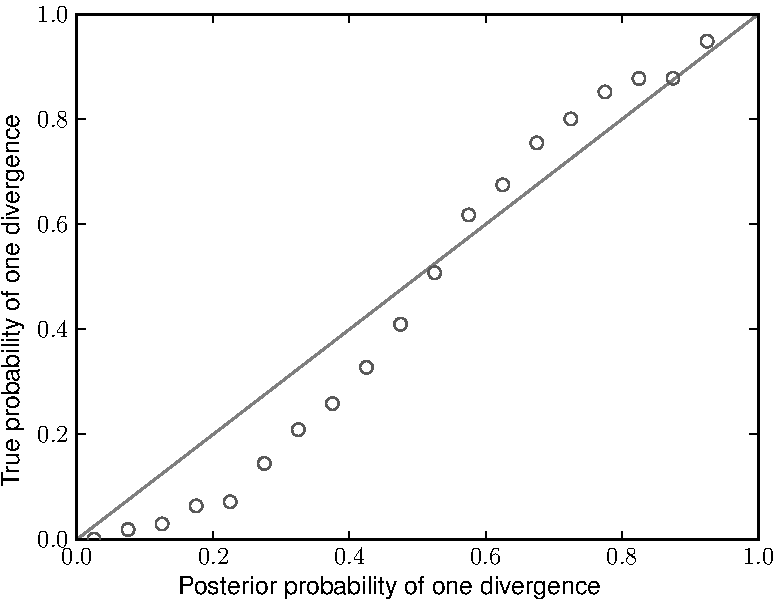
\includegraphics[height=7.0cm]{images/validation-model-choice-old.pdf}}
\end{frame}

\begin{frame}[t]
    \frametitle{Causes of bias: Marginal likelihoods}
    \vspace{1cm}
        \centerline{
        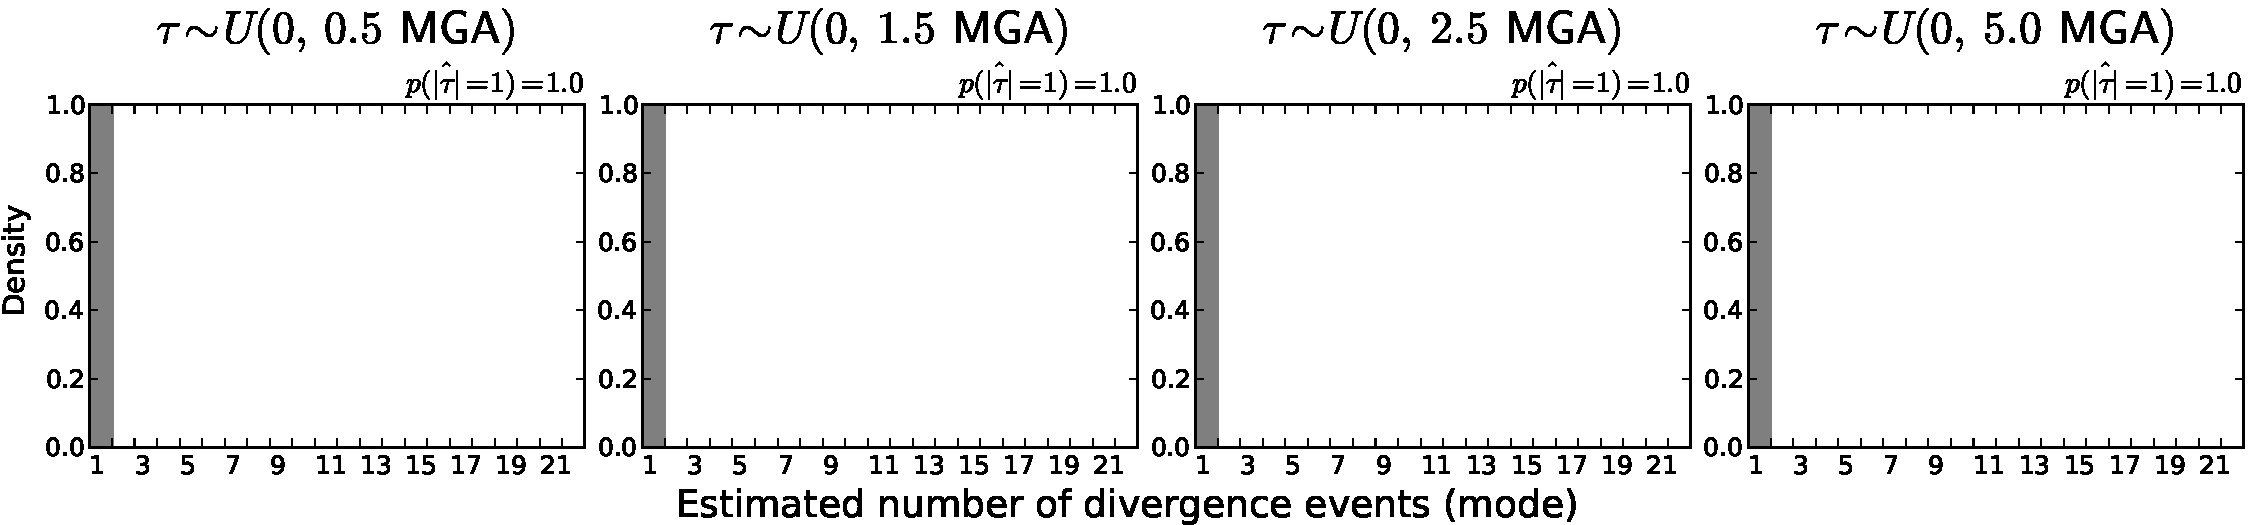
\includegraphics[width=\textwidth]{images/old-sims_power_psi_mode.pdf}}
        \vspace{0mm}
        \centerline{
        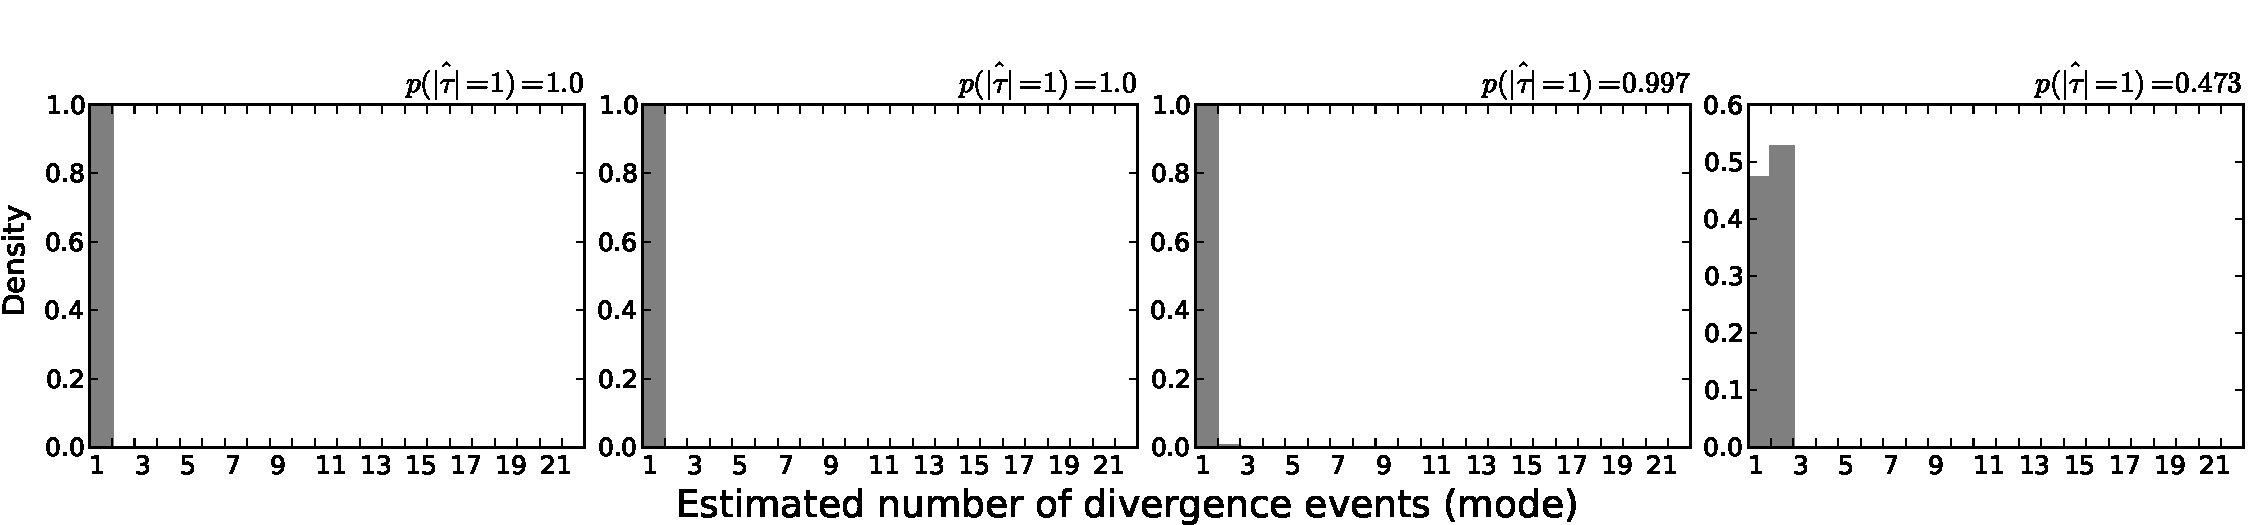
\includegraphics[width=\textwidth]{images/old-sims-inform10_power_psi_mode_headless.pdf}}
\end{frame}

\begin{frame}[t]
    \frametitle{Causes of bias: Marginal likelihoods}
    \vspace{1cm}
        \centerline{
        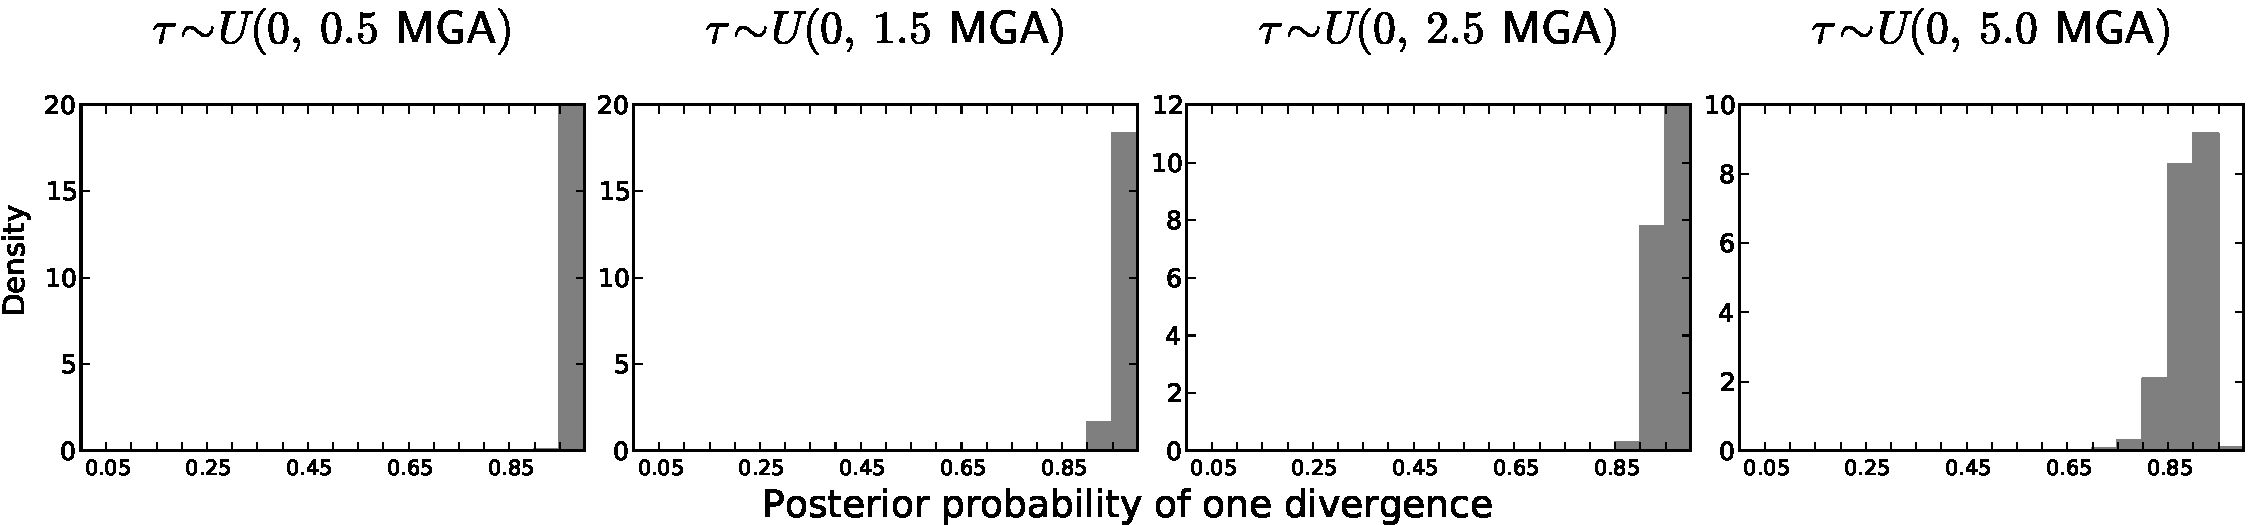
\includegraphics[width=\textwidth]{images/old-sims_power_psi_prob.pdf}}
        \vspace{0mm}
        \centerline{
        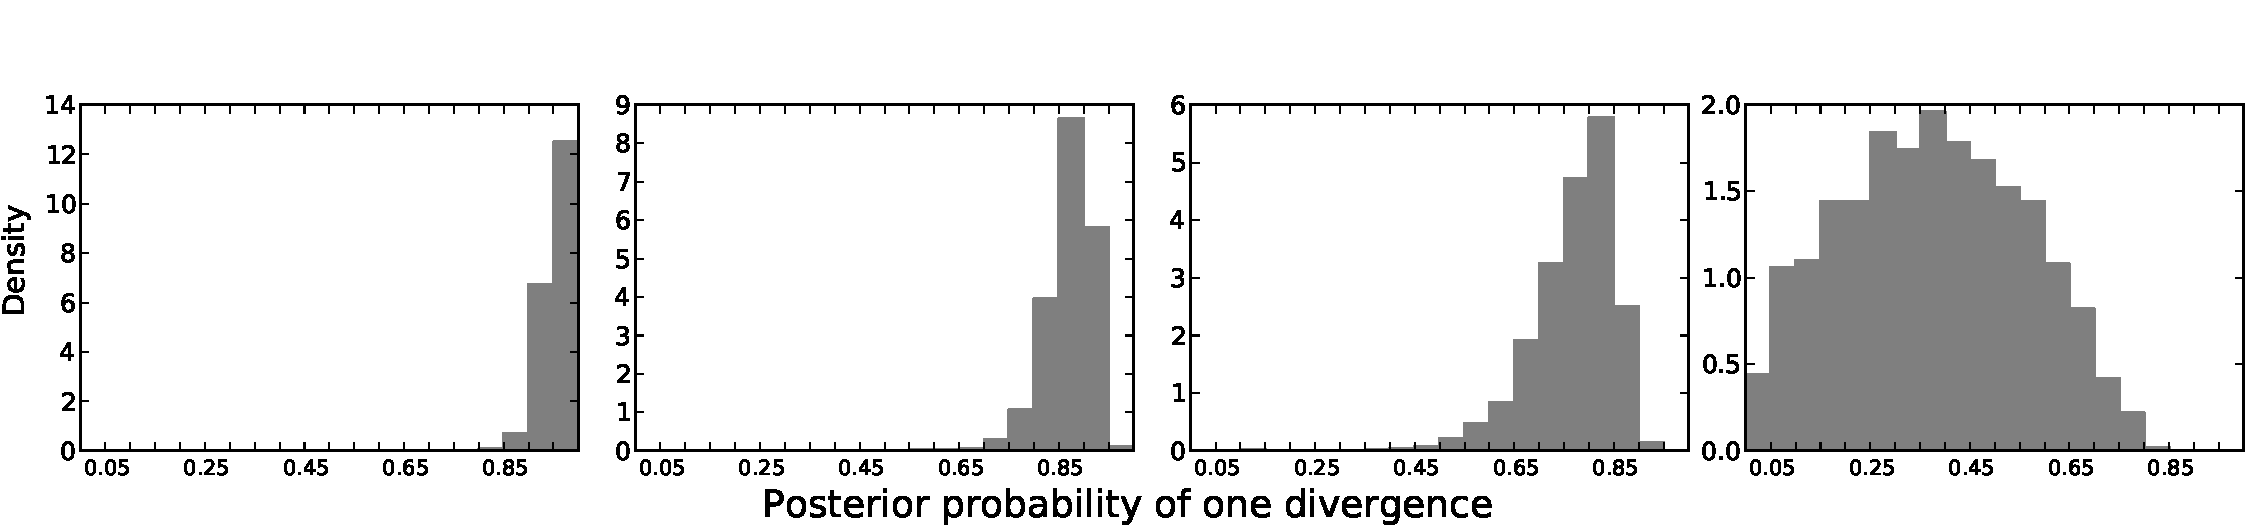
\includegraphics[width=\textwidth]{images/old-sims-inform10_power_psi_prob_headless.pdf}}
\end{frame}

\begin{frame}
    \frametitle{Causes of bias: Marginal likelihoods}
    Marginal likelihoods are at least partially responsible for bias\\
    \bigskip
    However, when uniform priors are narrower than possible in a real-world
    setting, the bias remains
    \bigskip
    \begin{block}<2>{\it Potential solution:}
        Use more flexible parametric distributions on nuisance parameters
        (e.g., gamma and beta)
    \end{block}
\end{frame}

\begin{frame}[t]
    \frametitle{Causes of bias: Marginal likelihoods}
    \begin{block}{\it Potential solution:}
        Use more flexible parametric distributions on nuisance parameters
        (e.g., gamma and beta)
    \end{block}
    \smallskip
    \centerline{
        \includegraphics<1>[height=6.0cm]{images/marginal-plot-2d-uniform-prior.pdf}
        \includegraphics<2>[height=6.0cm]{images/marginal-plot-2d.pdf}
        \includegraphics<3>[width=\textwidth]{images/partition_numbers.pdf}}
    \begin{block}<4>{\it Potential solution:}
        Use alternative prior over divergence models
        (e.g., uniform or Dirichlet process)
    \end{block}
\end{frame}

% \begin{frame}
%     \frametitle{Causes of bias: Theoretical limits of ABC}
%     When summary statistics are insufficient for discriminating among models,
%     ABC is inconsistent estimator of model posterior probabilities
%     \footlessfullcite{Robert2011}\\
%     \bigskip
%     True even if statistics are sufficient for each model\\
% \end{frame}

\begin{frame}
    \frametitle{New method: \dppmsbayes}
    \begin{itemize}
        \item Explain modifications: reparameterization, new prirors on nuisance parameters\ldots
        \item Uniform and DPP priors over divergence models
        \item Introduce DPP?
    \end{itemize}
\end{frame}

\begin{frame}
    \frametitle{\dppmsbayes: Model-choice results}
    \centerline{
        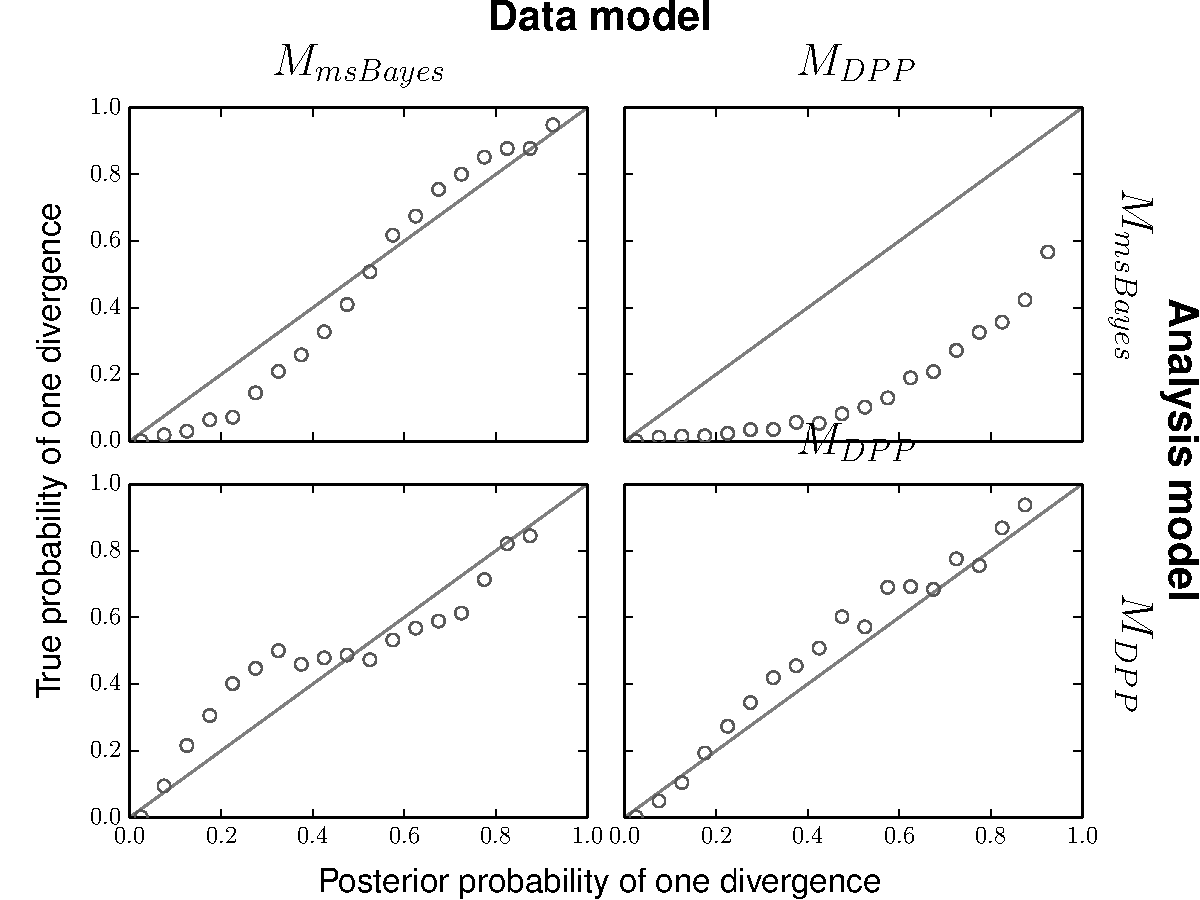
\includegraphics[height=7.0cm]{images/validation-model-choice-old-dpp.pdf}}
\end{frame}

\begin{frame}
    \frametitle{\dppmsbayes: Model-choice results}
    \centerline{
        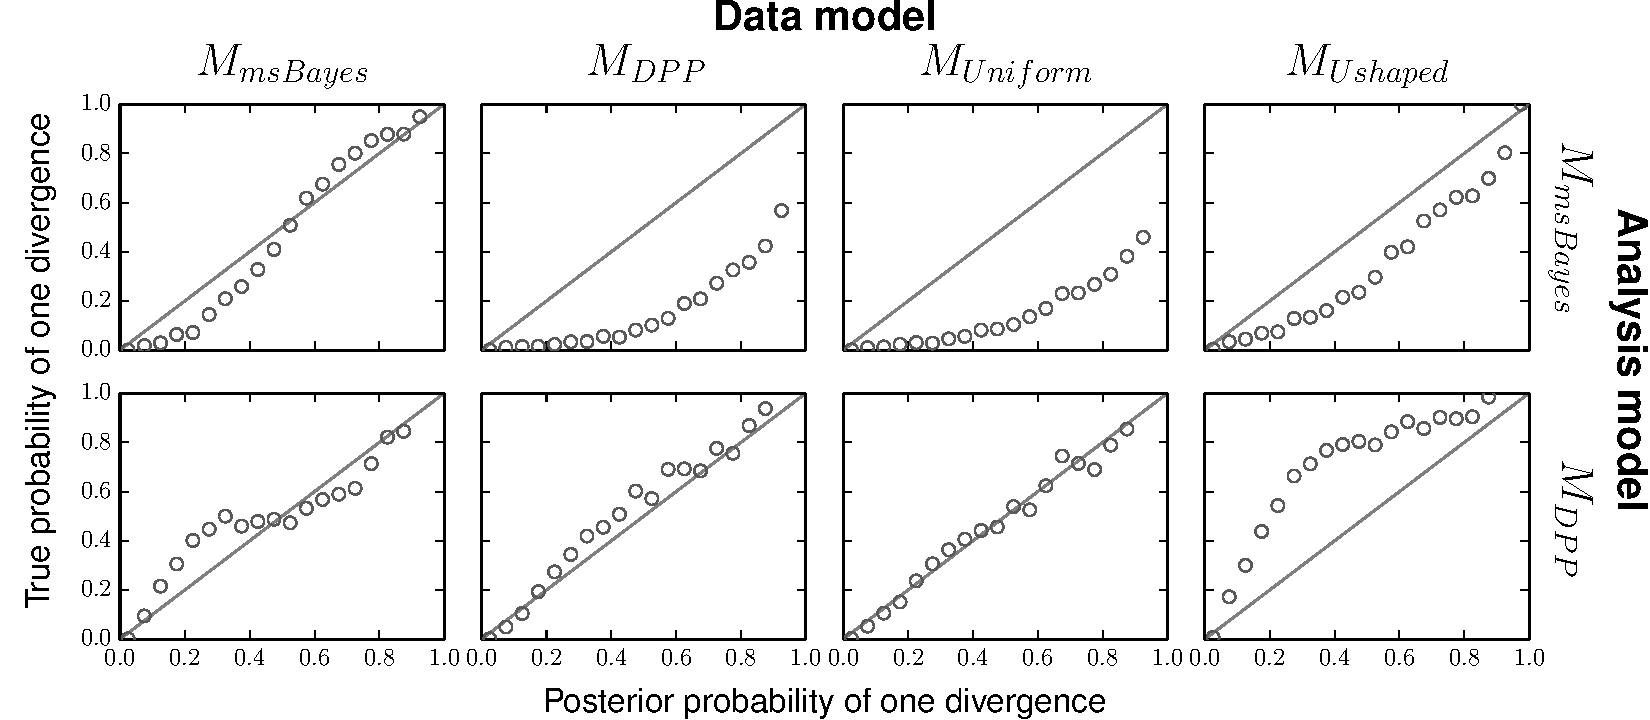
\includegraphics[width=1.13\textwidth]{images/validation-model-choice-old-dpp-full.pdf}}
\end{frame}

\begin{frame}[t]
    \frametitle{\dppmsbayes: Power results}
    \vspace{1cm}
        \centerline{
        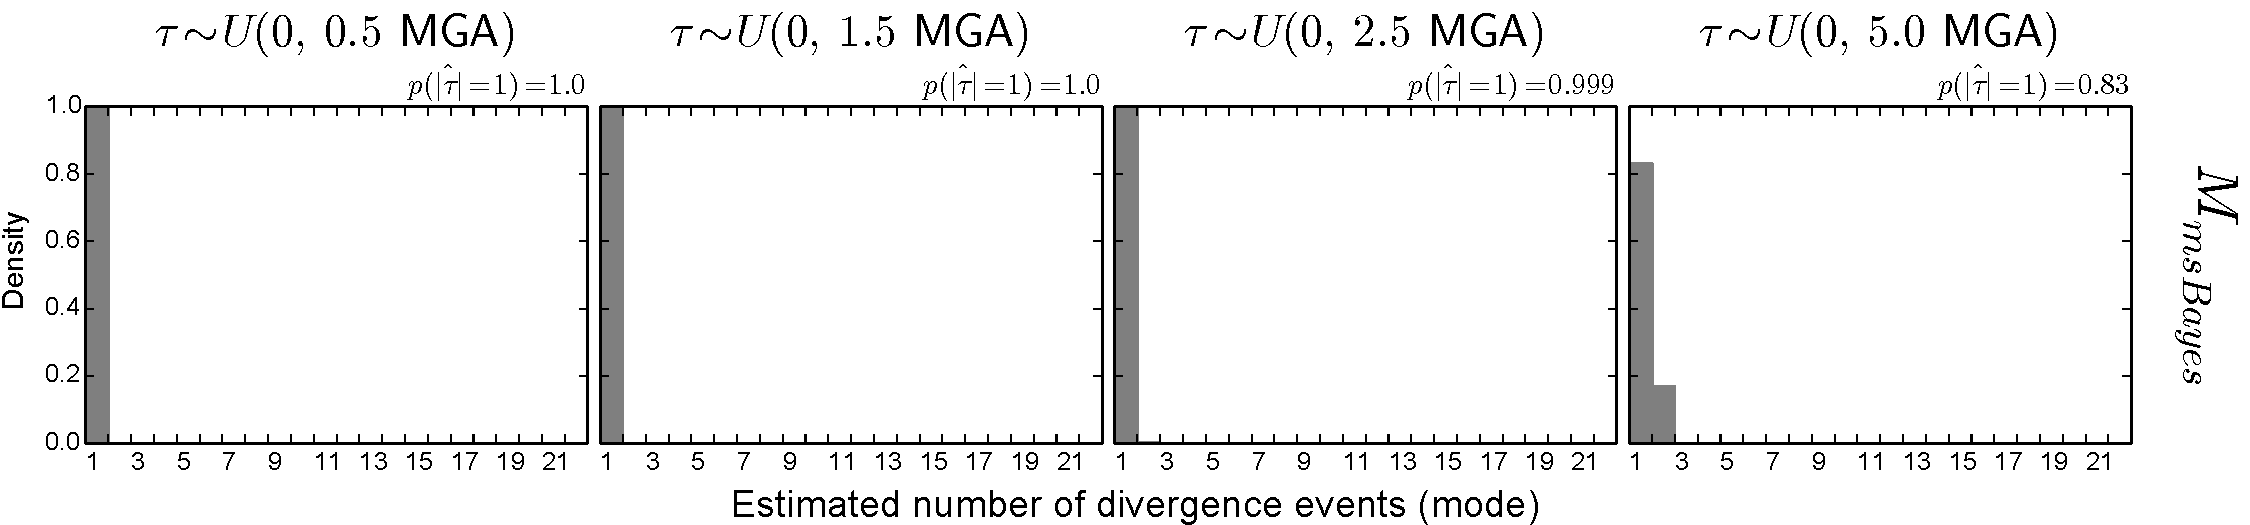
\includegraphics[width=1.13\textwidth]{images/old_old_power_psi_mode.pdf}}
        \vspace{0mm}
        \centerline{
        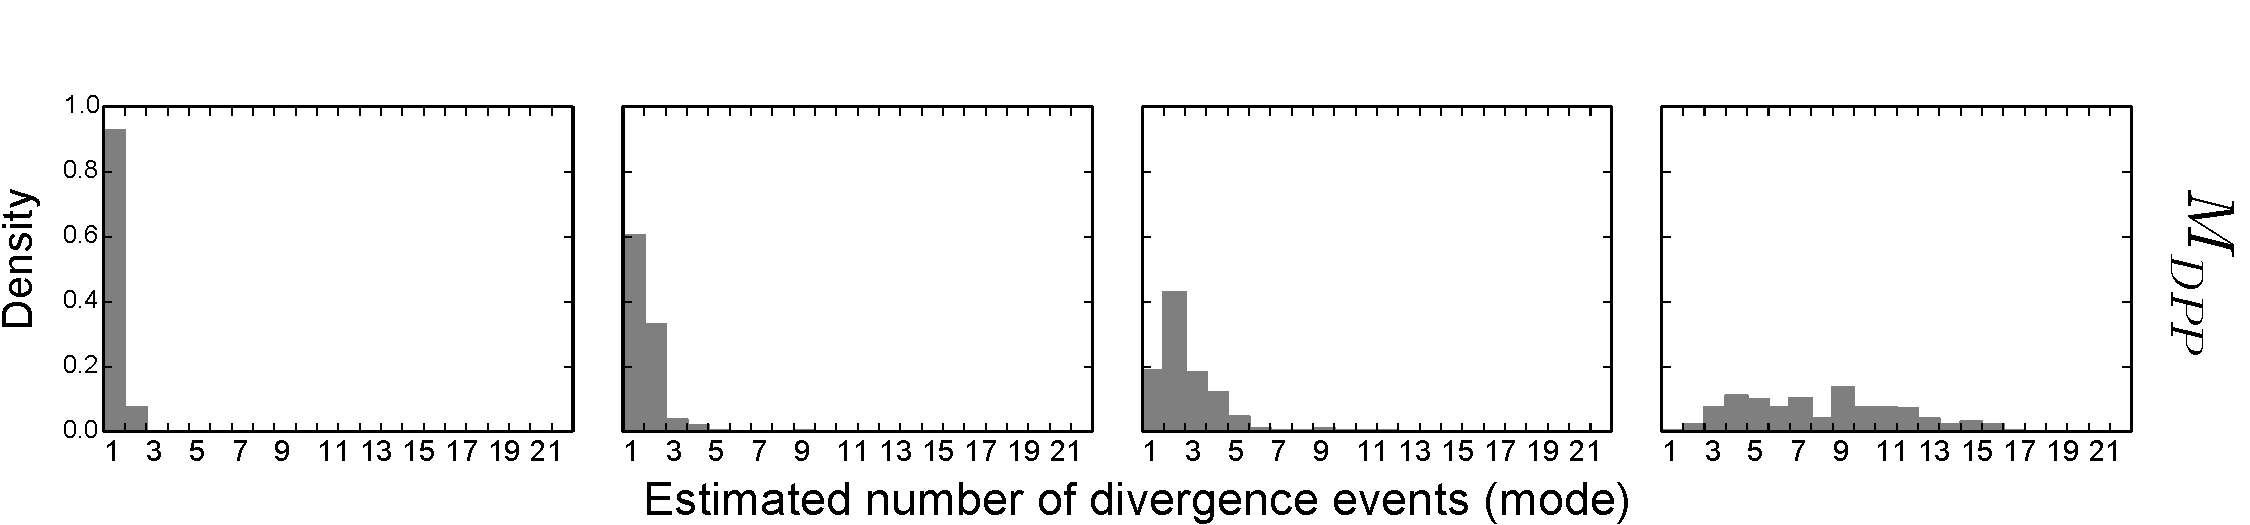
\includegraphics[width=1.13\textwidth]{images/old_dpp_power_psi_mode_headless.pdf}}
\end{frame}

\begin{frame}[t]
    \frametitle{\dppmsbayes: Power results}
    \vspace{1cm}
        \centerline{
        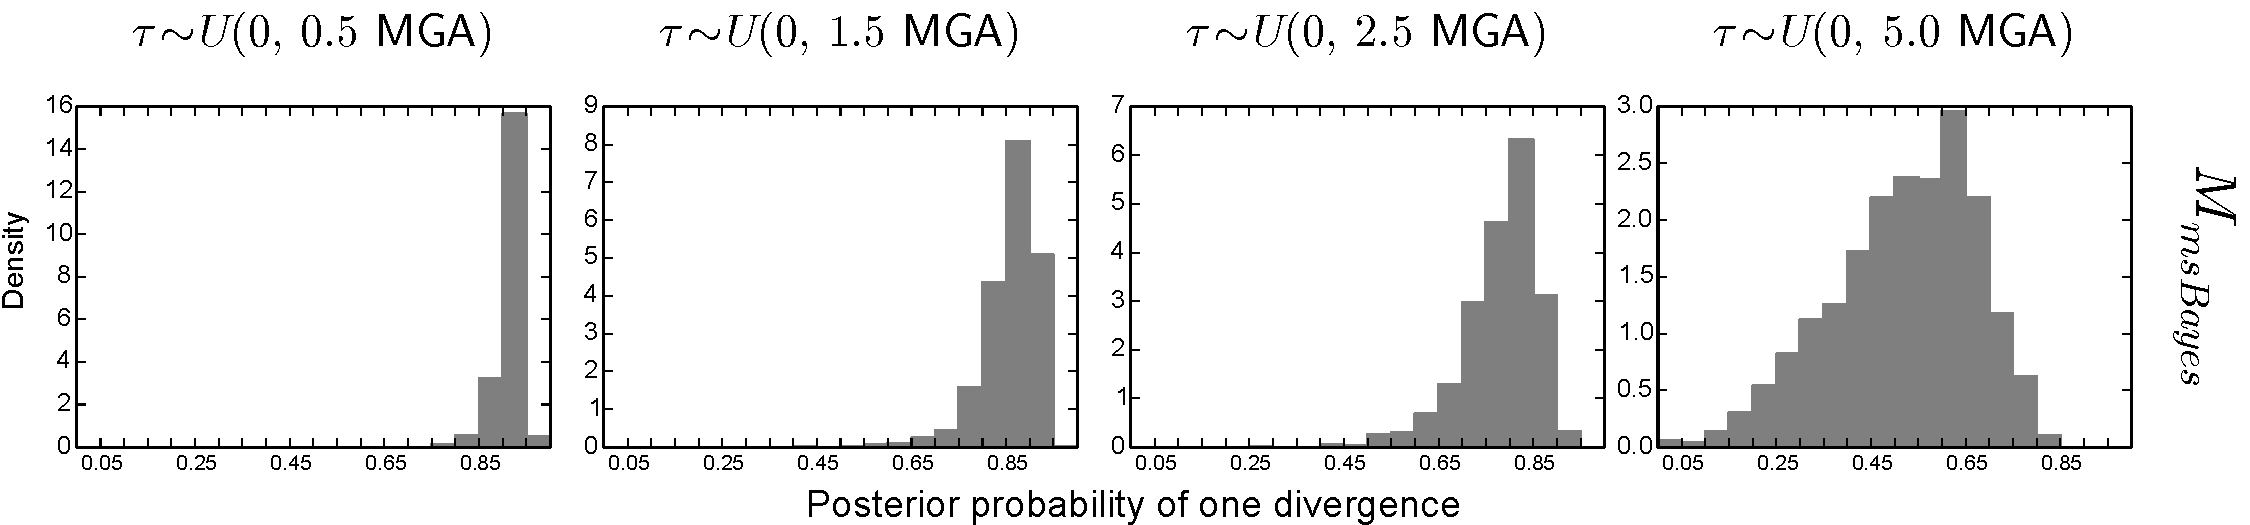
\includegraphics[width=1.13\textwidth]{images/old_old_power_psi_prob.pdf}}
        \vspace{0mm}
        \centerline{
        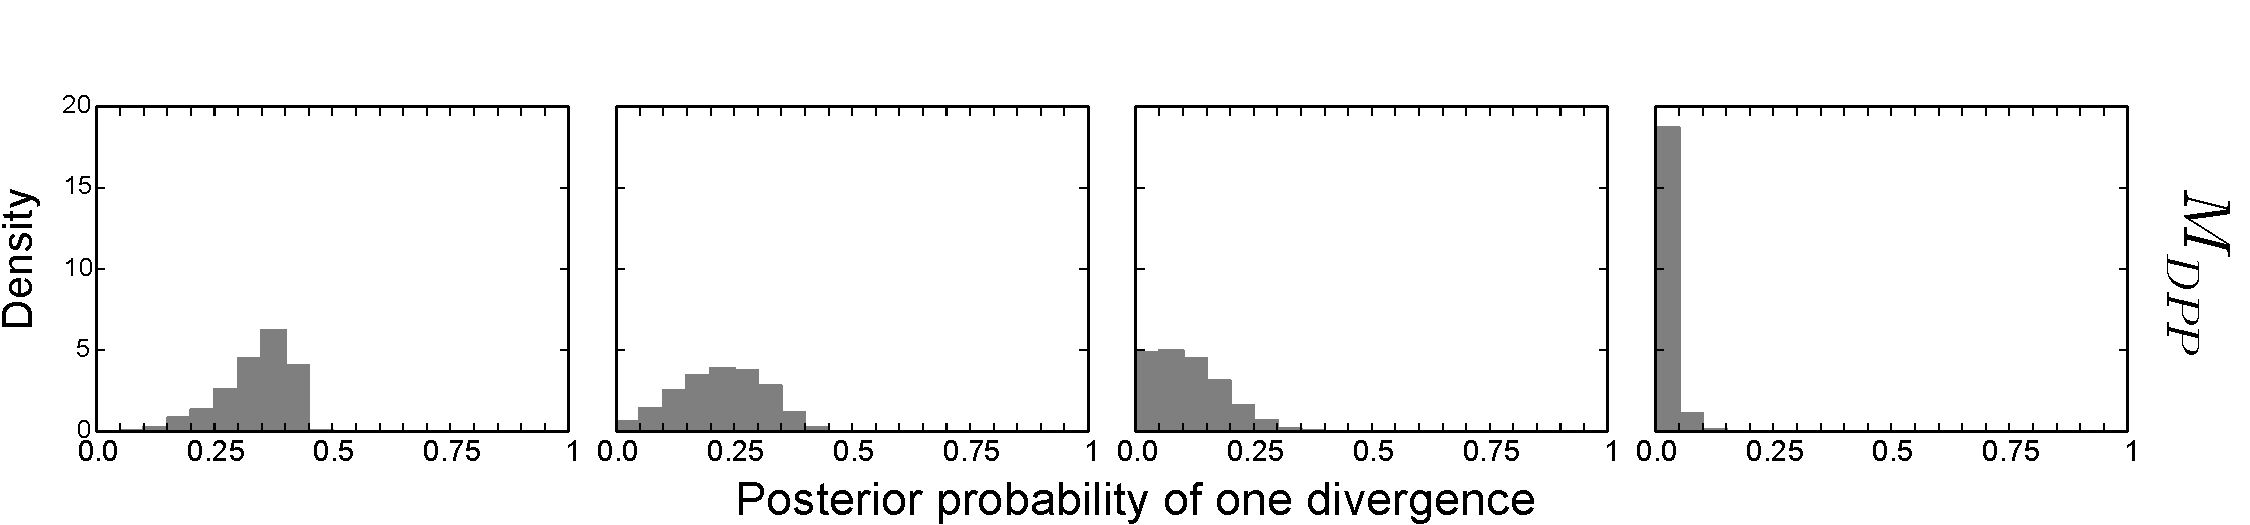
\includegraphics[width=1.13\textwidth]{images/old_dpp_power_psi_prob_headless.pdf}}
\end{frame}

\begin{frame}[t]
    \frametitle{\dppmsbayes: Power results}
    \vspace{1cm}
        \centerline{
        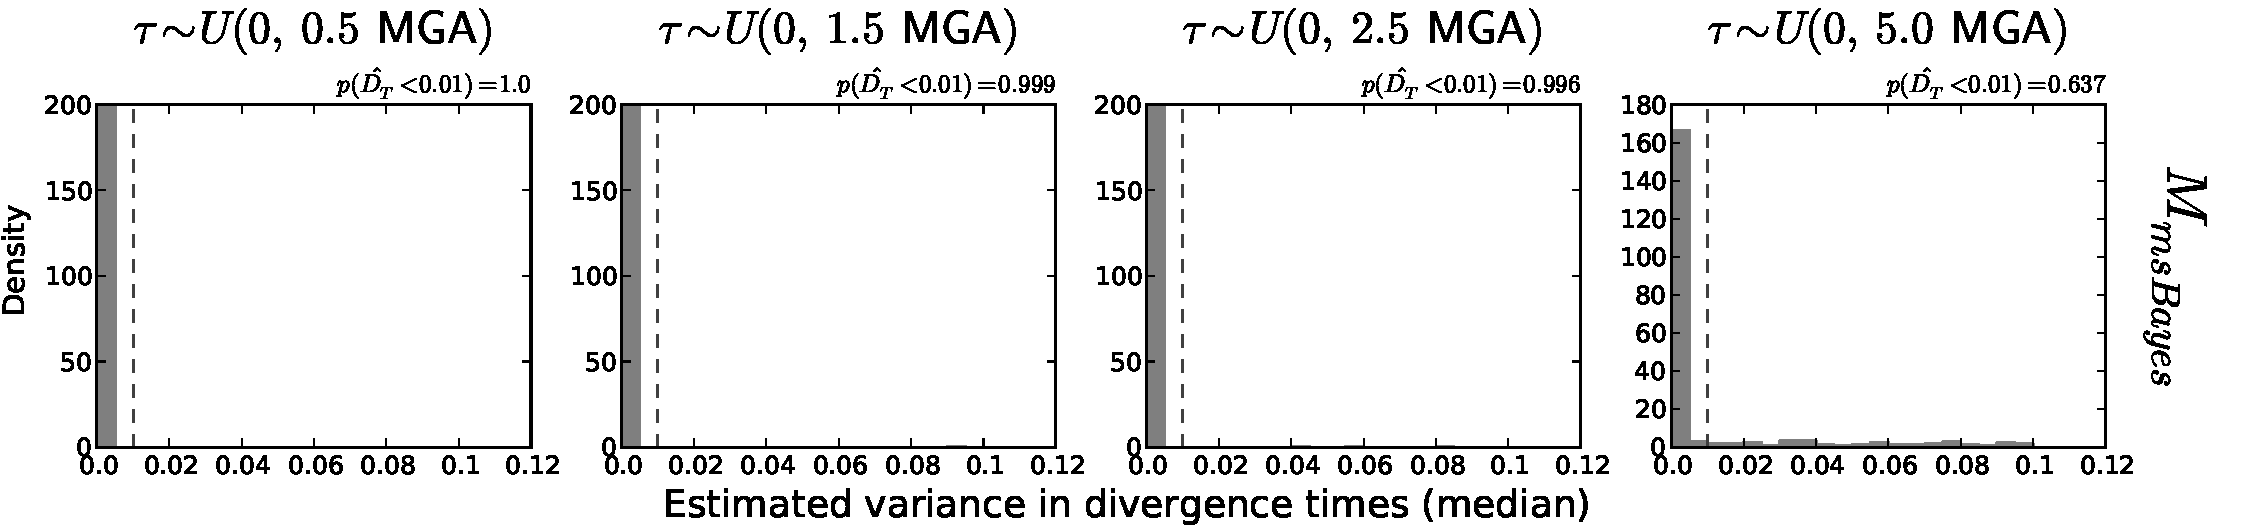
\includegraphics[width=1.13\textwidth]{images/old_old_power_omega_median.pdf}}
        \vspace{0mm}
        \centerline{
        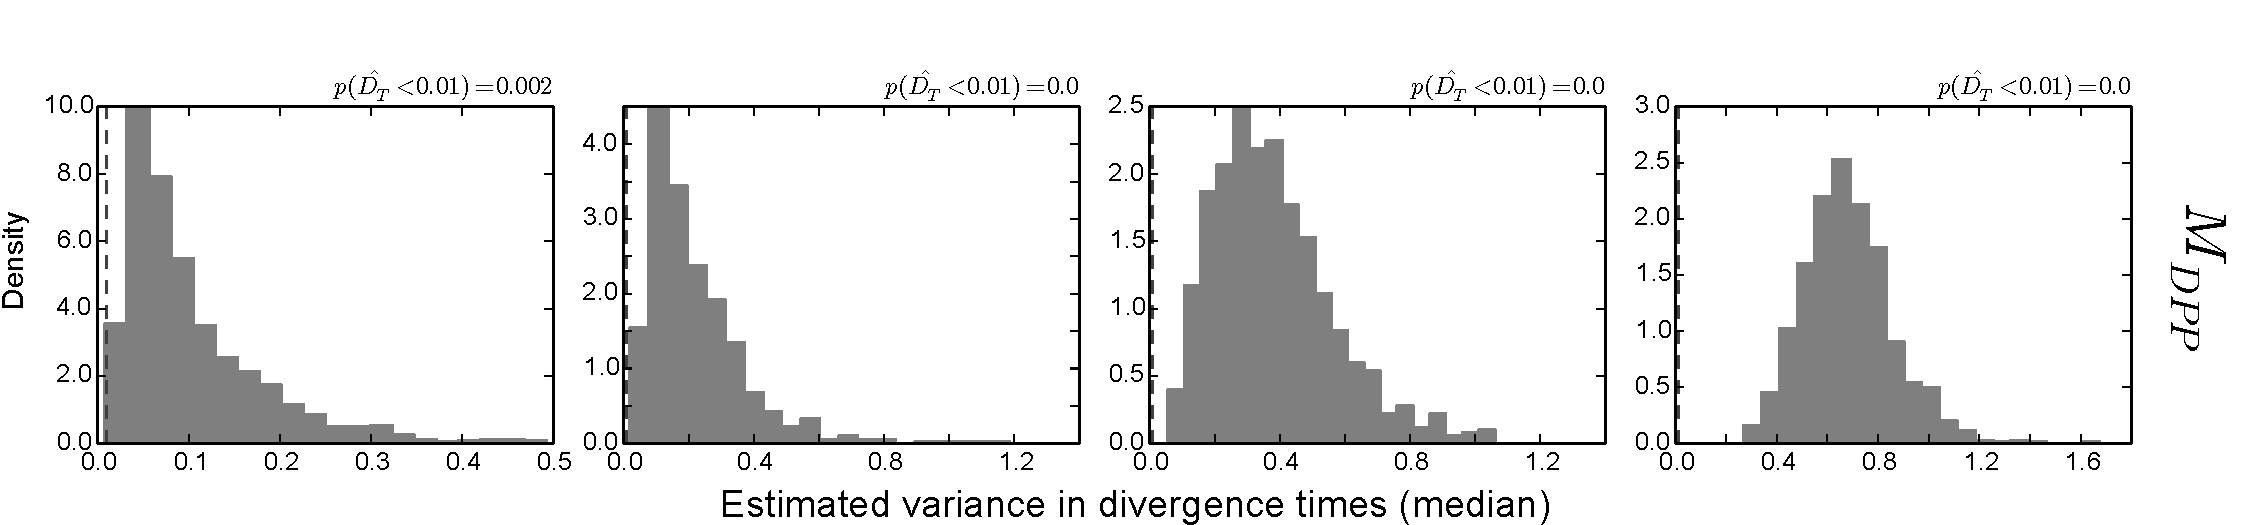
\includegraphics[width=1.13\textwidth]{images/old_dpp_power_omega_median_headless.pdf}}
\end{frame}

\begin{frame}
    \frametitle{\dppmsbayes: Power results}
    % \vspace{1cm}
        \centerline{
        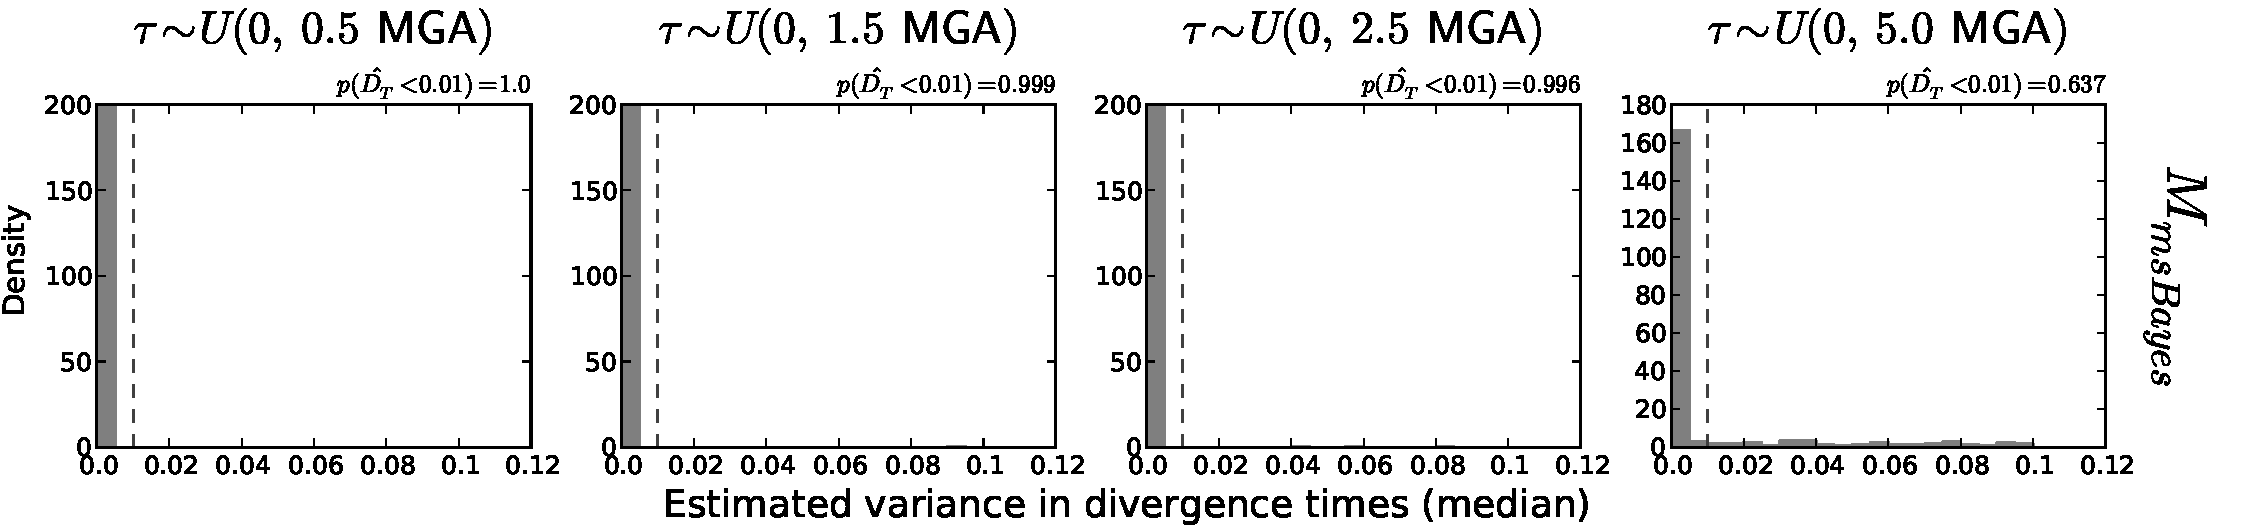
\includegraphics[width=\textwidth]{images/old_old_power_omega_median.pdf}}
        \vspace{0mm}
        \centerline{
        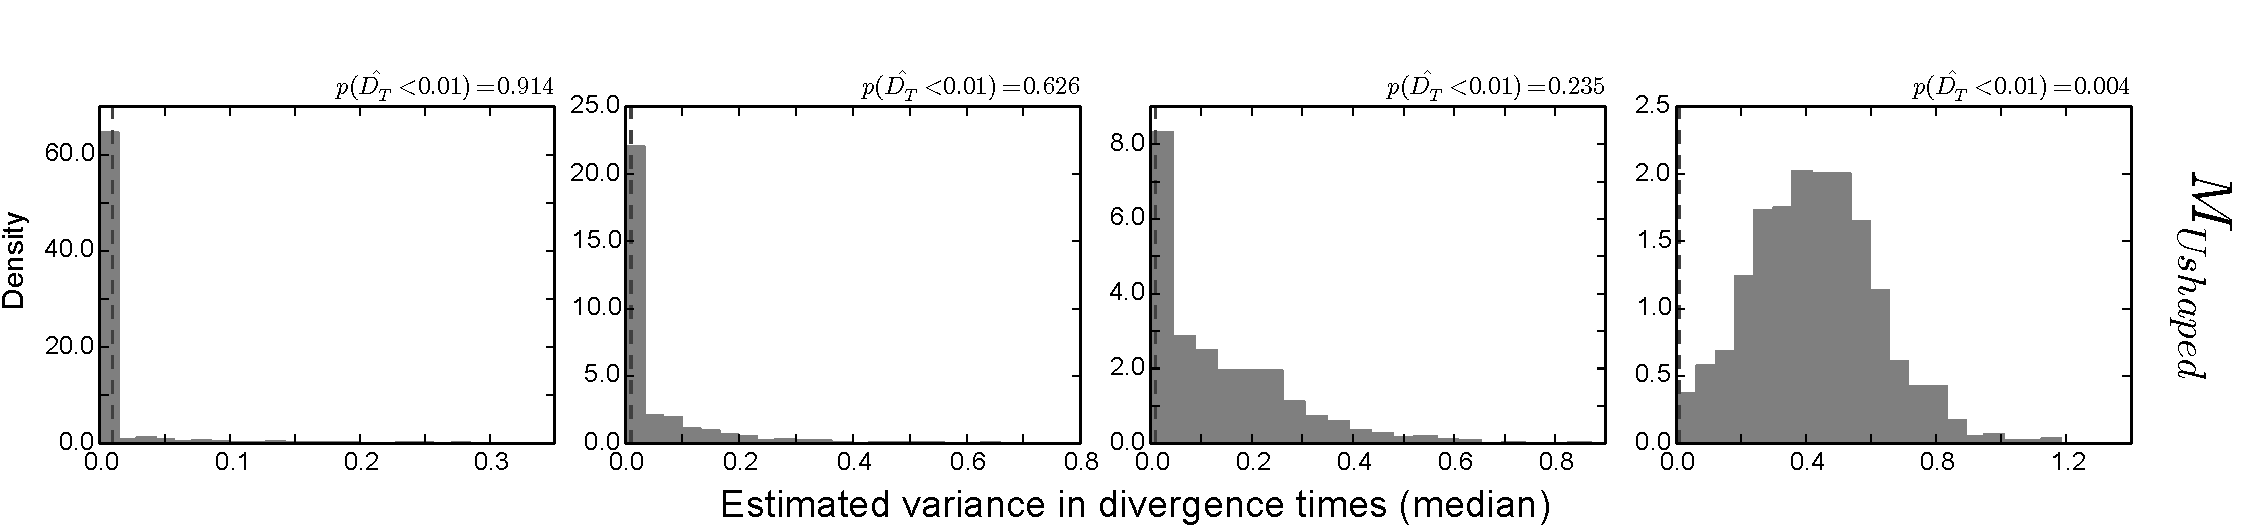
\includegraphics[width=\textwidth]{images/old_u-shaped_power_omega_median_headless.pdf}}
        \vspace{0mm}
        \centerline{
        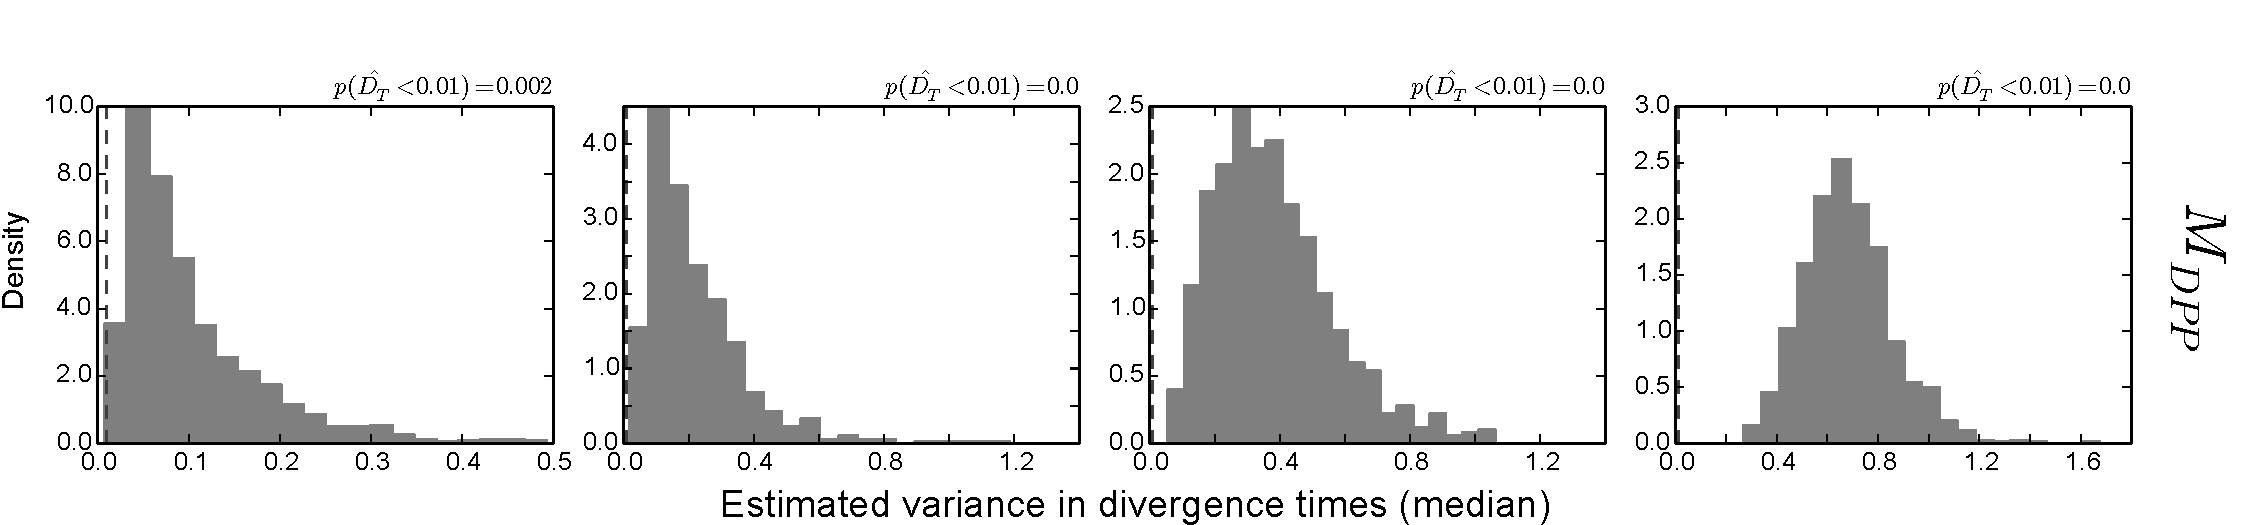
\includegraphics[width=\textwidth]{images/old_dpp_power_omega_median_headless.pdf}}
\end{frame}

\section{Conclusions}

\begin{frame}
\frametitle{Outline}
\tableofcontents[currentsection,currentsubsection]
\end{frame}

\begin{frame}
    \frametitle{Conclusions}
    Empirical results strongly support PAIC model \\
    \bigskip
    Based on simulations this is likely spurious \\
    \bigskip
    Low power and bias preclude any biological interpretation \\
    \bigskip
    Bias likely caused by combination of uniform priors on nuisance parameters
    and prior on model classes \\
    \bigskip
    \begin{block}{\it Potential Solutions:}
        \begin{enumerate}
            \item Flexible parametric distributions on nuisance parameters (e.g., gamma)
            \item More uniform prior over models (e.g., Dirichlet process)
        \end{enumerate}
    \end{block}
\end{frame}

\begin{frame}
    \frametitle{Recommendations}
    For Bayesian model choice, choose prior distributions carefully\\
    \bigskip
    All ABC model choice estimates should be accompanied by:
    \begin{enumerate}
        \item Simulation-based power analyses
        \item Assessment of prior sensitivity
    \end{enumerate}
    \medskip
\end{frame}

\section{An improved approach to the problem}

\begin{frame}
    \frametitle{PAIC model: Still needs testing}
    \begin{columns}[c]
        \column{.5\textwidth}
            What now? \\
            \begin{enumerate}
                \item Methodological advancements
                \begin{enumerate}
                    \item Extend \msb
                    \item Develop new fully Bayesian method
                \end{enumerate}
                \item Collect more data
            \end{enumerate}
        \column{.5\textwidth}
            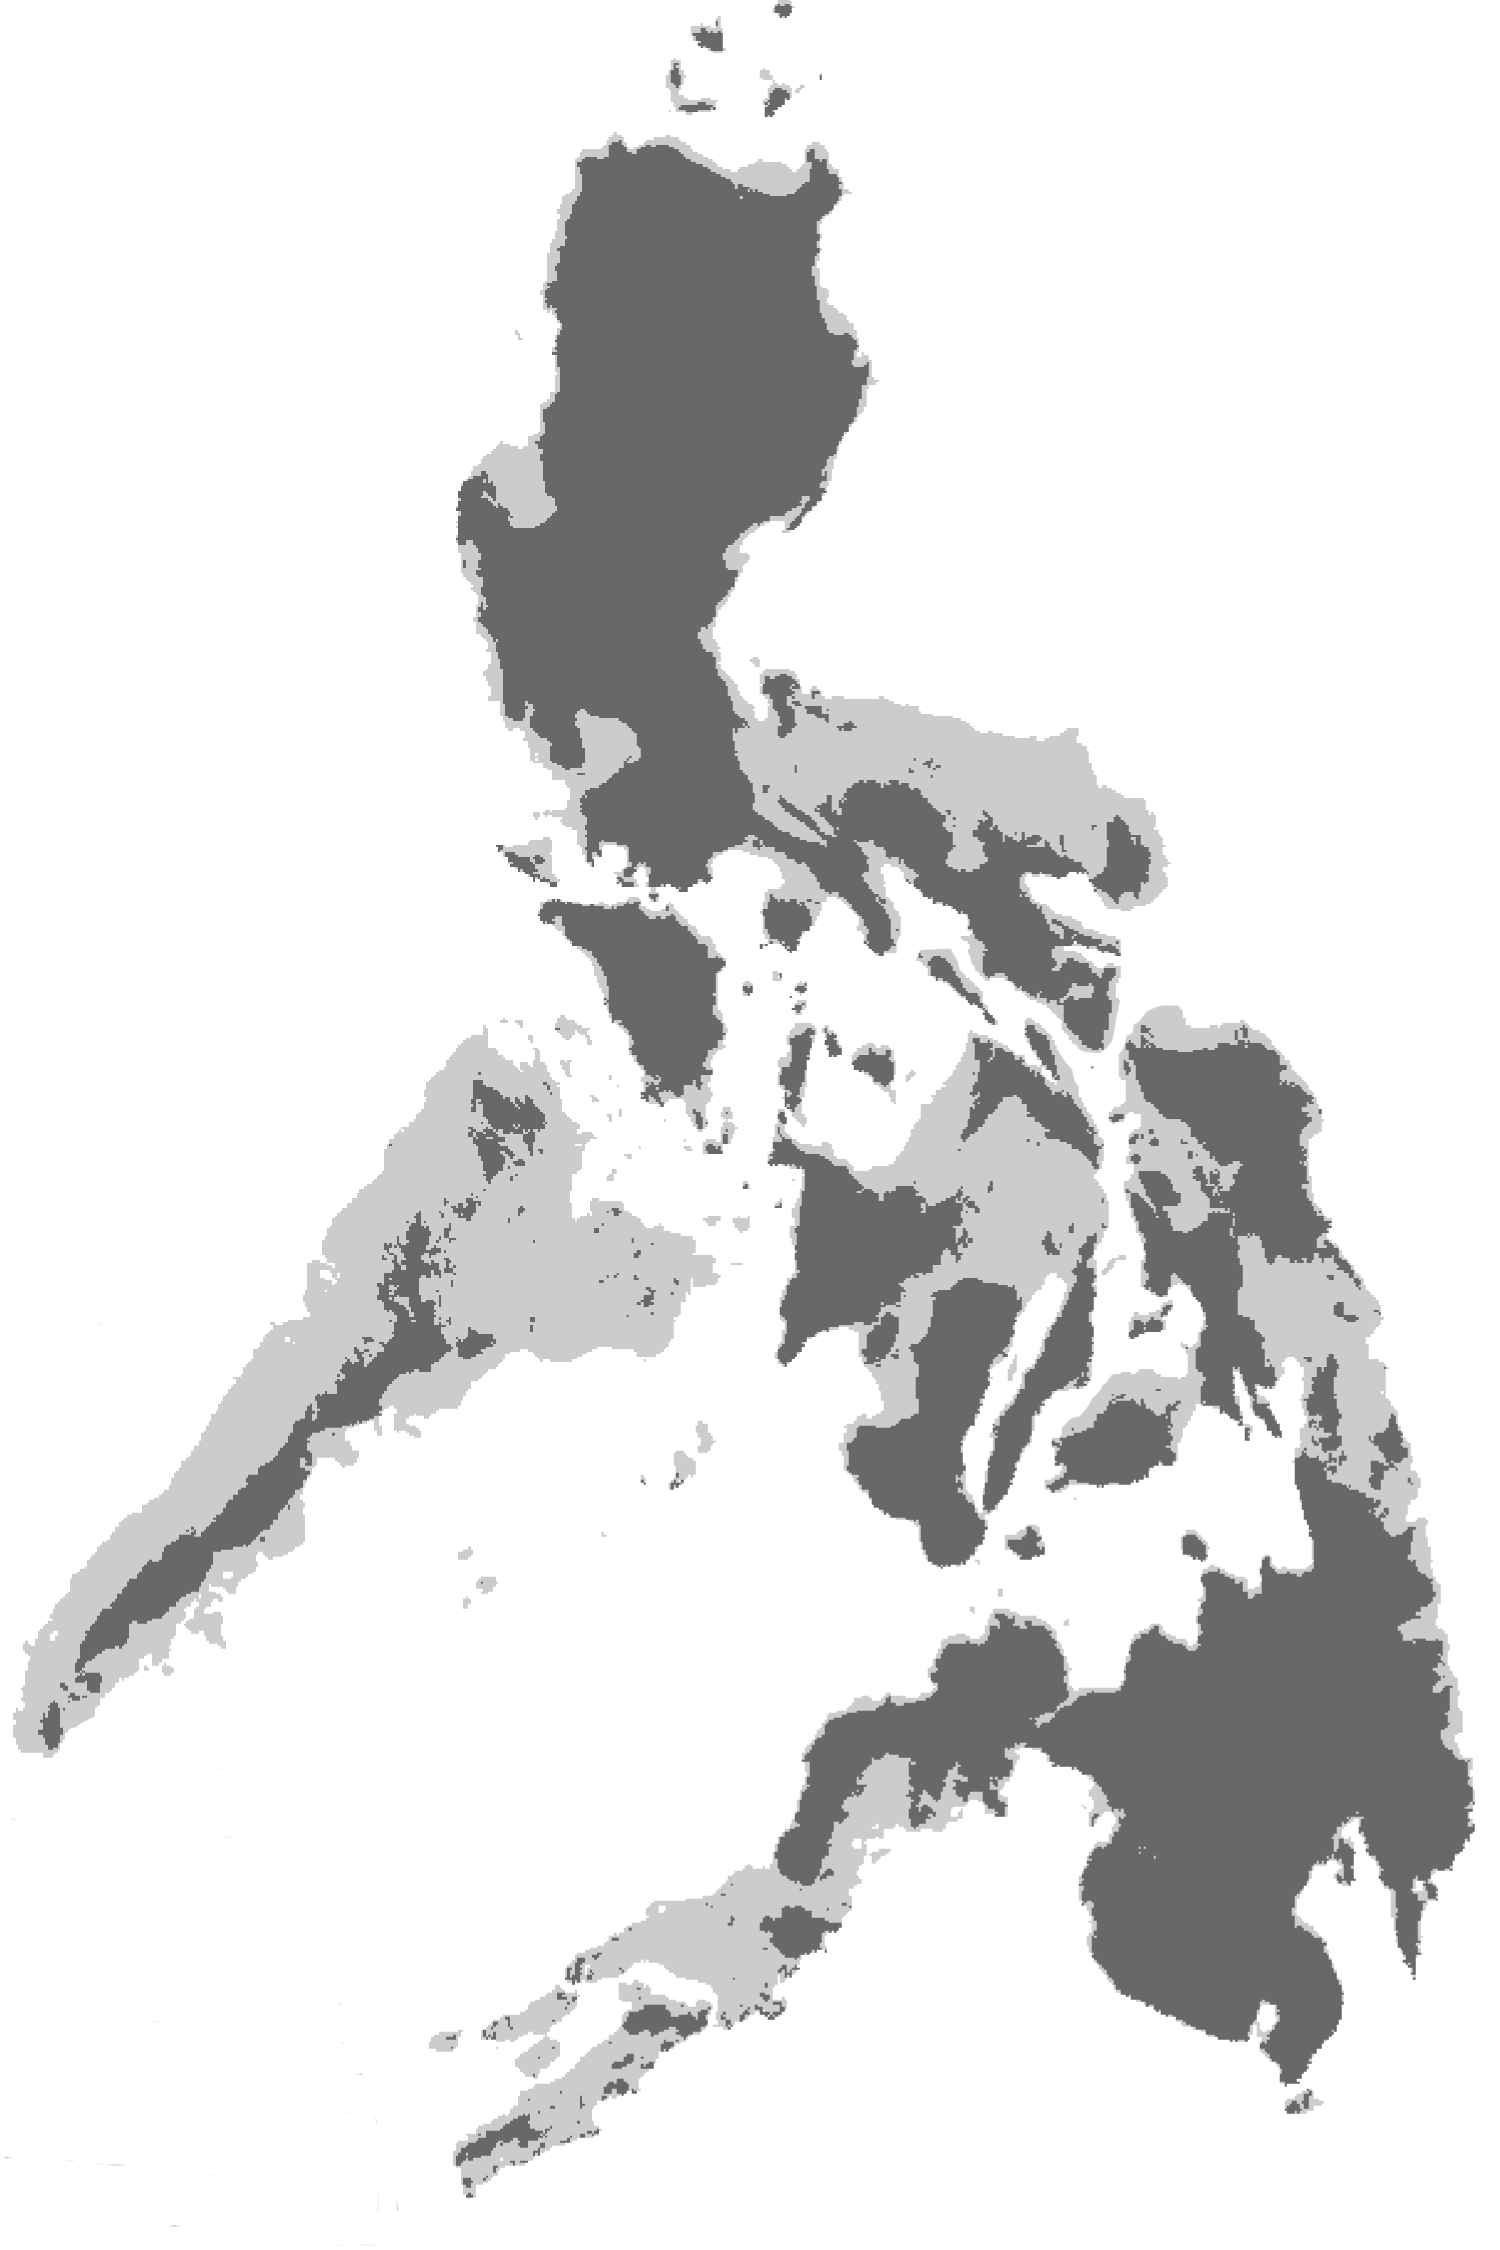
\includegraphics[width=\textwidth]{images/maps/Philippines.png}
    \end{columns}
\end{frame}

\subsection{Improving existing and developing new method}

\begin{frame}
    \frametitle{Extend \msb}
    \begin{myitemize}
        \item Implement flexible prior options for demographic parameters
        \item Implement a better prior over divergence models
        \begin{enumerate}
            \item Uniform prior over divergence models (rather than \numt{})
            \item Dirichlet process prior
        \end{enumerate}
    \end{myitemize}
\end{frame}

\begin{frame}
    \frametitle{Novel Bayesian method}
    \includegraphics<1>[width=\textwidth]{images/model-cartoon-masked.pdf}
    \includegraphics<2>[width=\textwidth]{images/model-cartoon.pdf}
\end{frame}

\subsection{More data---a lot more}

\begin{frame}
    \frametitle{Genomic data}
    \begin{columns}[c]
        \column{.5\textwidth}
        \begin{myitemize}
            \item Collecting genomic data from two gekkonid radiations
                co-distributed throughout most of Philippine Archipelago
            \begin{myitemize}
                \item \emph{Cyrtodactylus}---12 species
                \item \emph{Gekko}---13 species
            \end{myitemize}
            \item Whole genome assemblies for each genus
            \item RAD-seq libraries constructed for $\sim130$ individuals
                from each genus
        \end{myitemize}
        \column{.5\textwidth}
        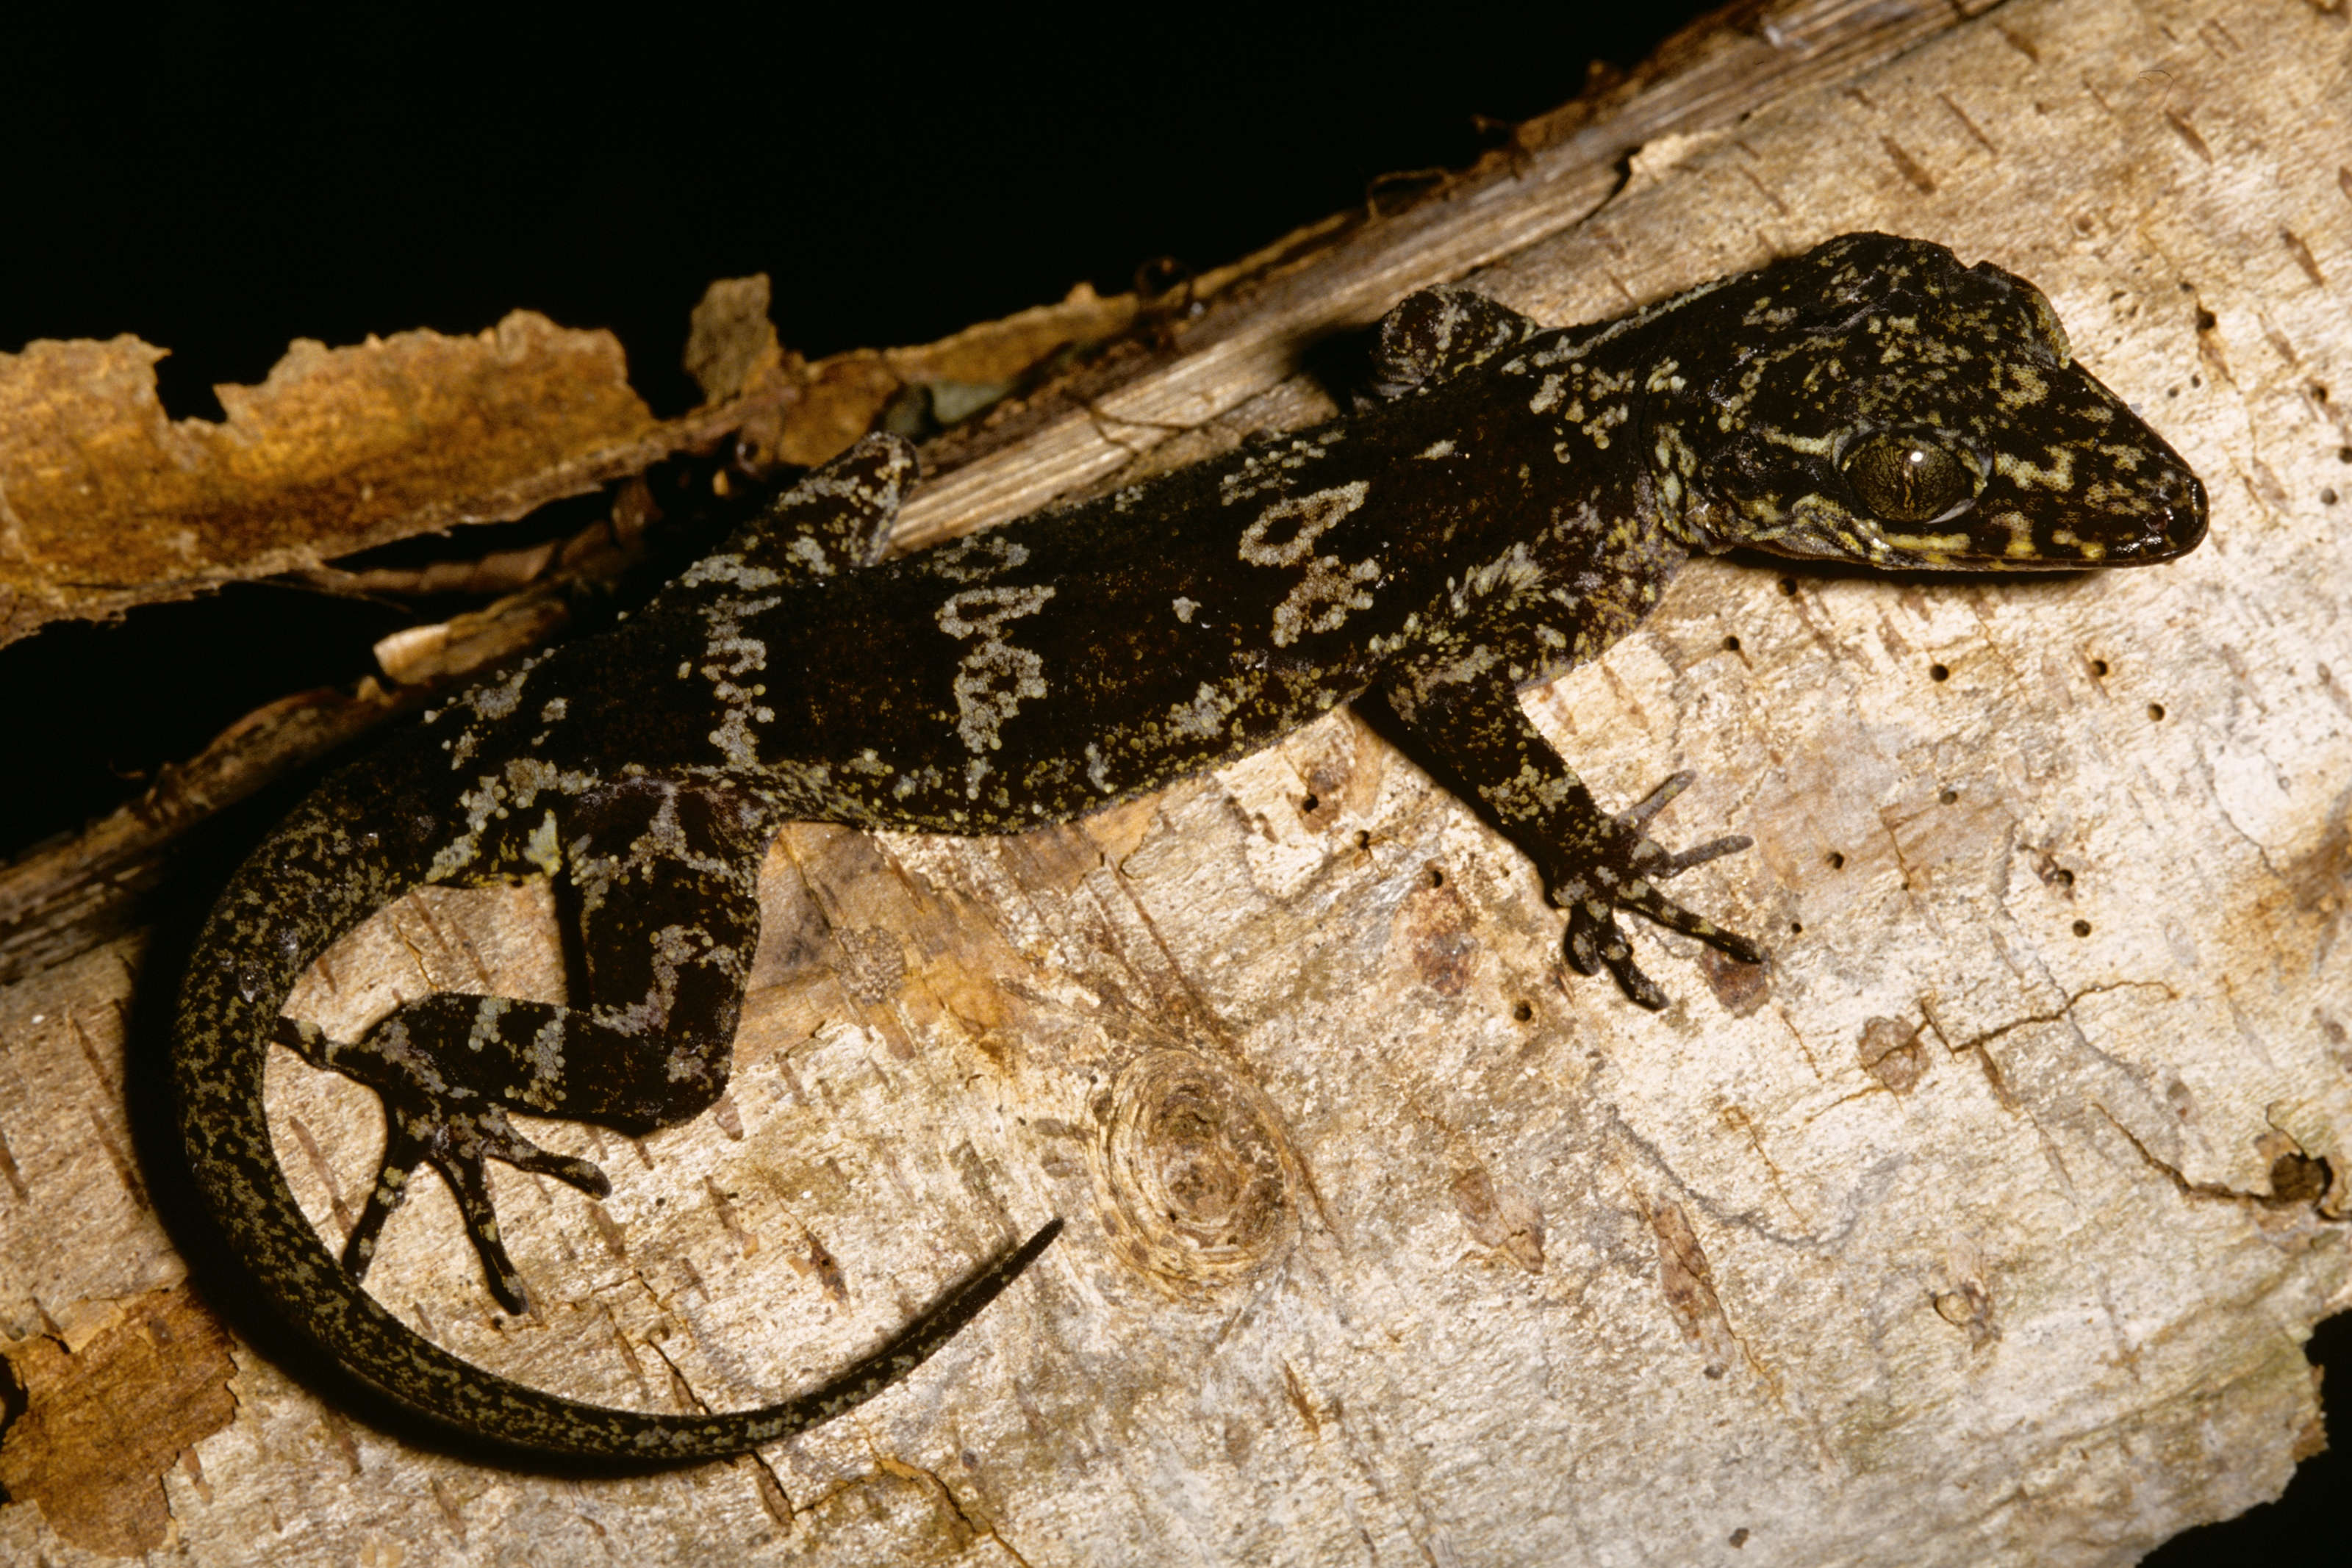
\includegraphics[width=\textwidth]{images/photos/cyrt-agusanensis.jpg} \quad
        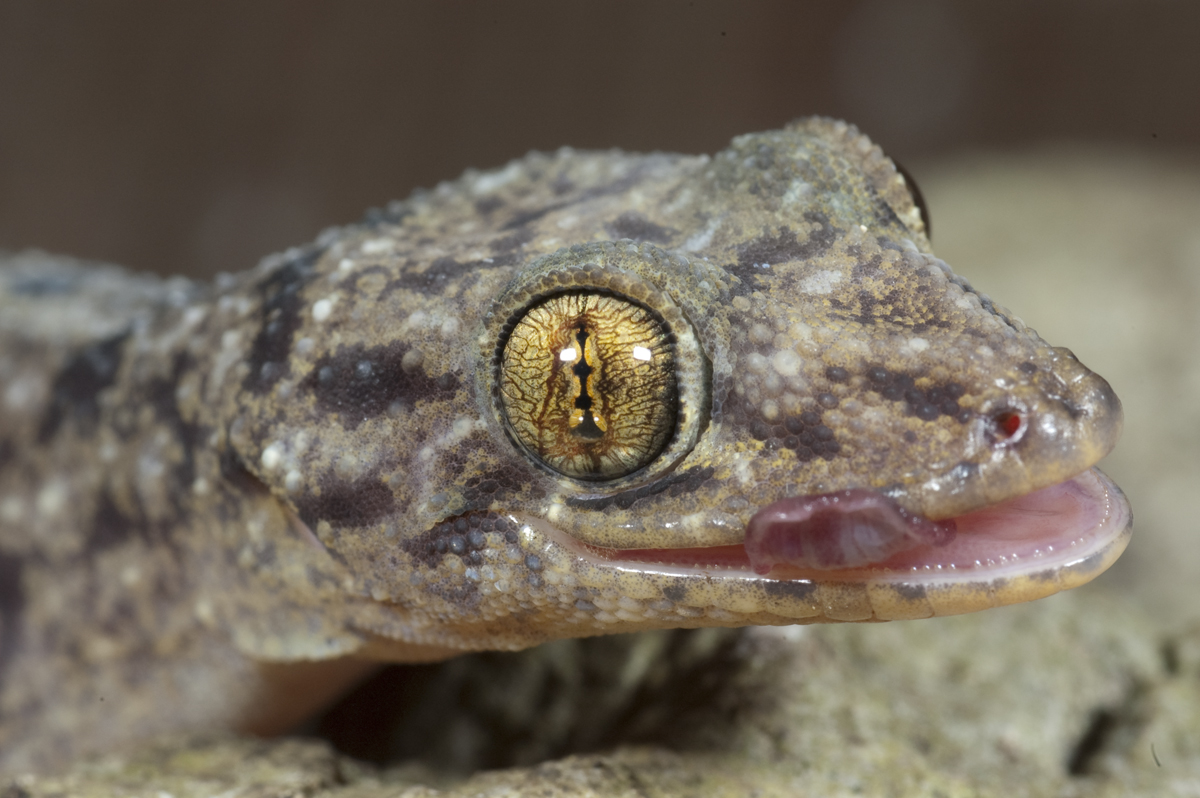
\includegraphics[width=\textwidth]{images/photos/gekko-mindorensis.jpg}
    \end{columns}
\end{frame}


\begin{frame}
    \frametitle{Acknowledgments}
    \begin{columns}[c]
        \column{.5\textwidth}
            {\bf Ideas and feedback:}
            \begin{myitemize}
                \item KU Herpetology
                \item Holder Lab
                \item Melissa Callahan
                \item Mike Hickerson
                \item Laura Kubatko
            \end{myitemize}
        \column{.5\textwidth}
            {\bf Funding:}
            \begin{myitemize}
                \item NSF
                \item KU EEB \& BI
            \end{myitemize}
            {\bf Computation:}
            \begin{myitemize}
                \item KU ITTC
                \item KU Computing Center
            \end{myitemize}
    \end{columns}
\end{frame}

% Extra slides

\begin{frame}[noframenumbering]
    \frametitle{Geological history}
    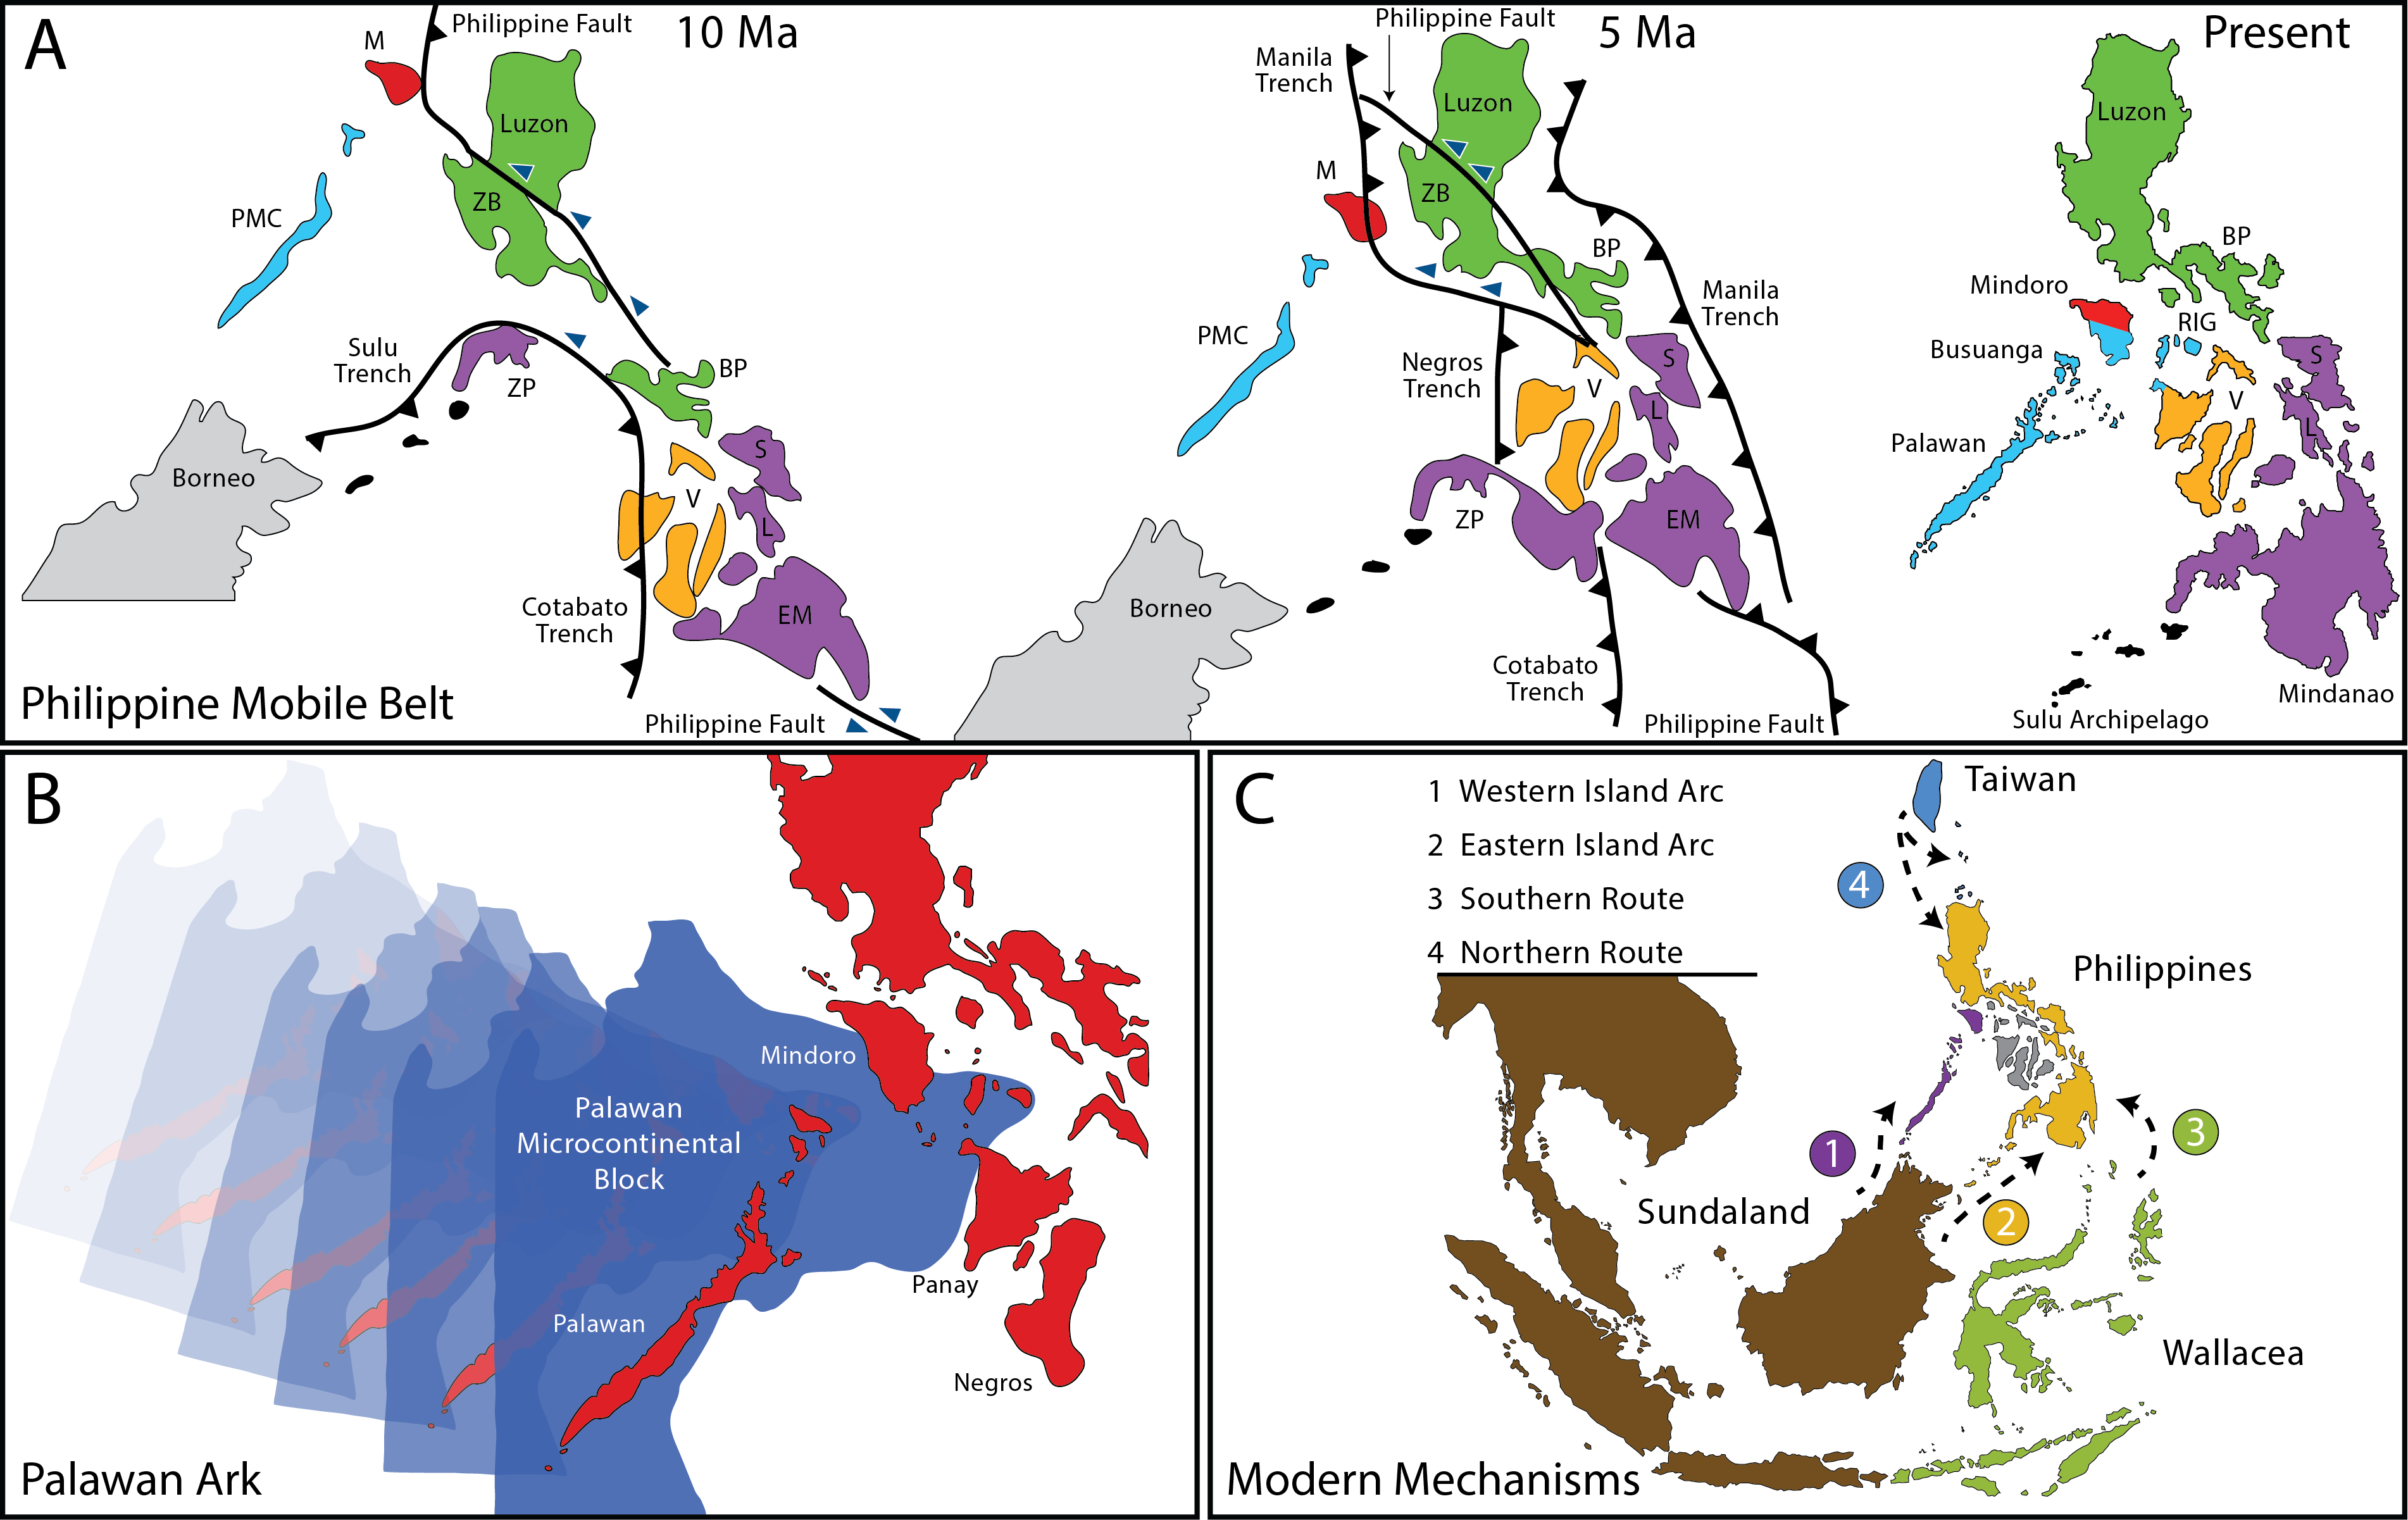
\includegraphics[width=\textwidth]{images/maps/arees-fig3.png}
\end{frame}
    
\begin{frame}[noframenumbering]
    \frametitle{Gene tree divergences}
    \centerline{
    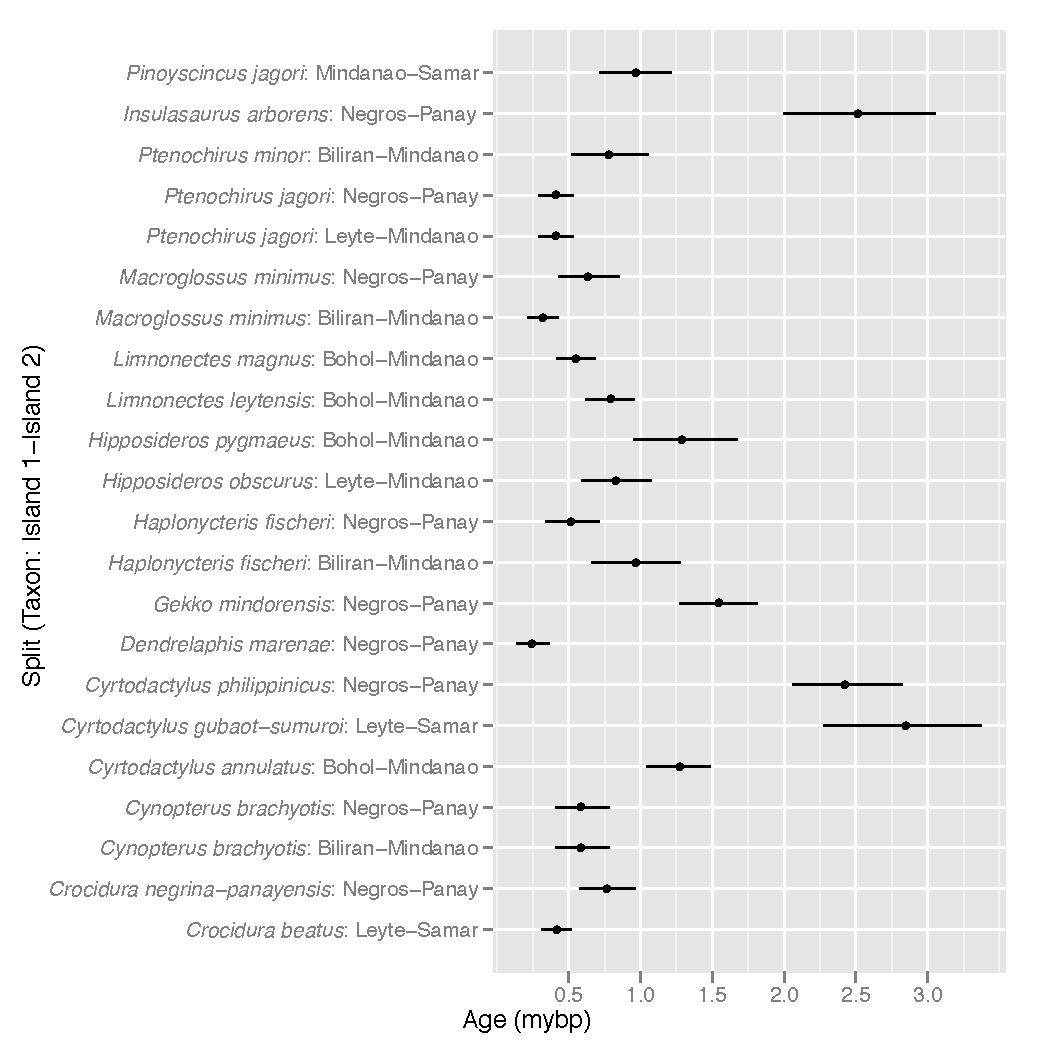
\includegraphics[height=8cm]{images/gene_splits.pdf}}
\end{frame}

\end{document}

